\documentclass[12pt, letterpaper]{article}

% --- Paquetes de configuración ---
\usepackage[utf8]{inputenc}
\usepackage[T1]{fontenc}
\usepackage[spanish, es-tabla]{babel} % Español
\usepackage{amsmath} % Para matemáticas avanzadas
\usepackage{geometry}
\geometry{left=3cm, right=3cm, top=3cm, bottom=3cm} % Márgenes estándar
\usepackage{graphicx} % Para imágenes
\usepackage{float}    % Para posicionamiento exacto de figuras con [H]
\usepackage{tikz}     % Para el marco azul
\usetikzlibrary{calc}
\usepackage{enumitem} % Para listas personalizadas
\usepackage{hyperref} % Para enlaces en la ToC
\usepackage{titlesec} % Para formato de títulos
\usepackage{xltabular} % Para tablas que se dividen en varias páginas
\usepackage{ragged2e} % Para justificar texto en tablas

% --- Importar definiciones de métricas ---
% ============================================================================
% METRICS DEFINITIONS - CHAMPION MODEL (exp_05 XGBoost)
% Auto-generated from JSON metadata - DO NOT HARDCODE VALUES
% Last updated: 2026-04-15
% ============================================================================

% Cross-Validation Performance Metrics
\newcommand{\championROCAUC}{0.6391}
\newcommand{\championROCAUCstd}{0.0371}
\newcommand{\championBrierScore}{0.2672}

% Operating Point Performance Metrics (Test Set)
\newcommand{\championRecall}{0.8647}
\newcommand{\championSpecificity}{0.2854}
\newcommand{\championPrecision}{0.3634}
\newcommand{\championNPV}{0.8172}
\newcommand{\championFOneScore}{0.5118}
\newcommand{\championFTwoScore}{0.6778}
\newcommand{\championAccuracy}{0.4711}
\newcommand{\championKappa}{0.1100}
\newcommand{\championOptimalThreshold}{0.48}
\newcommand{\championAveragePrecision}{0.5171}

% Confusion Matrix Values
\newcommand{\championTP}{326}
\newcommand{\championFP}{571}
\newcommand{\championTN}{228}
\newcommand{\championFN}{51}
\newcommand{\championTPpct}{86.47}
\newcommand{\championFPpct}{71.46}
\newcommand{\championTNpct}{28.54}
\newcommand{\championFNpct}{13.53}

% Model Information
\newcommand{\championModelName}{XGBoost}
\newcommand{\championExperiment}{exp\_05\_hyperparameter\_search}

% Experiment Evolution - AUC-ROC Progression
\newcommand{\expOneAUC}{0.6153}
\newcommand{\expOneBestModel}{CatBoost}
\newcommand{\expTwoAUC}{0.6235}
\newcommand{\expTwoBestModel}{CatBoost}
\newcommand{\expThreeAUC}{0.6134}
\newcommand{\expThreeBestModel}{CatBoost}
\newcommand{\expFourAUC}{0.6209}
\newcommand{\expFourBestModel}{CatBoost}
\newcommand{\expFiveAUC}{0.6391}
\newcommand{\expFiveBestModel}{XGBoost}

% Top 3 Feature Importances (XGBoost exp_05)
\newcommand{\topFeatureOne}{SANGRADO\_MAYOR}
\newcommand{\topFeatureOneImportance}{19.16}
\newcommand{\topFeatureTwo}{HB\_x\_SANGRADO}
\newcommand{\topFeatureTwoImportance}{13.73}
\newcommand{\topFeatureThree}{DIABETES}
\newcommand{\topFeatureThreeImportance}{10.11}

% Clinical Interpretation
\newcommand{\recallInterpretation}{El modelo detecta \championRecall\ (\championTPpct\%) de los casos de choque hemorrágico}
\newcommand{\npvInterpretation}{Valor predictivo negativo de \championNPV, indicando alta confianza cuando predice ausencia de choque}


% Configuración de enlaces (sin recuadros rojos)
\hypersetup{
    colorlinks=true,
    linkcolor=black,
    filecolor=magenta,      
    urlcolor=blue,
}

% Configuración de párrafos
\setlength{\parskip}{0.5em}
\setlength{\parindent}{1cm}

% Configuración de títulos centrados (solo secciones)
\usepackage{sectsty}
\sectionfont{\centering}

% Configuración de altura de celdas en tablas
\renewcommand{\arraystretch}{1.5}

\begin{document}

% -----------------------------------------------------------------------------
% PÁGINA 1: PORTADA
% -----------------------------------------------------------------------------
\begin{titlepage}
    % Marco Azul usando TikZ
    \begin{tikzpicture}[remember picture, overlay]
        \draw[blue!90!black, line width=4pt] 
            ($(current page.north west) + (1.5cm,-1.5cm)$) 
            rectangle 
            ($(current page.south east) + (-1.5cm,1.5cm)$);
    \end{tikzpicture}

    \centering
    
    % Logotipo Universidad ICESI
    
\includegraphics[width=0.4\textwidth]{images/image001.png} 
    
    \vspace{2cm}
    
    {\Large \textbf{Predicción temprana de shock hemorrágico en pacientes sometidos a cirugía mayor no cardiaca mediante modelos de inteligencia artificial}}
    
    \vspace{1.5cm}
    
    {\Large \textbf{Proyecto de Grado}}
    
    \vspace{2cm}
    
    \textbf{Autores:}\\
    Cristian Eduardo Botina Carpio\\
    Juan Manuel Marín Angarita\\
    Óscar Andrés Gómez Lozano
    
    \vspace{1cm}
    
    \textbf{Tutores:}\\
    Ángela Villota Gómez
    
    \vfill
    
    \textbf{Universidad Icesi}\\
    Facultad Barberi de Ingeniería, Diseño y Ciencias Aplicadas\\
    Ingeniería de Sistemas\\
    Santiago De Cali\\
    2025
    
\end{titlepage}

% -----------------------------------------------------------------------------
% PÁGINA 2: TABLA DE CONTENIDO
% -----------------------------------------------------------------------------

\tableofcontents
\newpage

% -----------------------------------------------------------------------------
% PÁGINA 3: LISTA DE ACRÓNIMOS
% -----------------------------------------------------------------------------
\section*{Lista de acrónimos}
\addcontentsline{toc}{section}{Lista de acrónimos}

\begin{description}[style=multiline, leftmargin=3.5cm, font=\bfseries]
    \item[ACS] Sociedad \textbf{A}mericana de \textbf{C}irujanos (\textbf{A}merican \textbf{C}ollege of \textbf{S}urgeons)
    \item[AUC-ROC] \textbf{Á}rea \textbf{B}ajo la \textbf{C}urva ROC (\textbf{A}rea \textbf{U}nder the \textbf{R}eceiver \textbf{O}perating \textbf{C}haracteristic Curve)
    \item[CO] Gasto \textbf{C}ardíaco (\textbf{C}ardiac \textbf{O}utput)
    \item[CV] \textbf{V}alidación \textbf{C}ruzada (\textbf{C}ross \textbf{V}alidation)
    \item[DCS] \textbf{C}irugía de \textbf{C}ontrol de \textbf{D}año (\textbf{D}amage \textbf{C}ontrol \textbf{S}urgery)
    \item[DNN] \textbf{R}edes \textbf{N}euronales \textbf{P}rofundas (\textbf{D}eep \textbf{N}eural \textbf{N}etworks)
    \item[DT] \textbf{Á}rbol de \textbf{D}ecisión (\textbf{D}ecision \textbf{T}ree)
    \item[FC] \textbf{F}recuencia \textbf{C}ardíaca
    \item[FVL] \textbf{F}undación \textbf{V}alle de \textbf{L}ili
    \item[GBM] \textbf{M}áquina de \textbf{R}efuerzo de \textbf{G}radiente (\textbf{G}radient \textbf{B}oosting \textbf{M}achine)
    \item[IA] \textbf{I}nteligencia \textbf{A}rtificial
    \item[IMC] \textbf{Í}ndice de \textbf{M}asa \textbf{C}orporal
    \item[IS] \textbf{Í}ndice de \textbf{S}hock
    \item[KNN] \textbf{K} vecinos más cercanos (\textbf{K} \textbf{N}earest \textbf{N}eighbors)
    \item[LightGBM] \textbf{M}áquina de \textbf{R}efuerzo de \textbf{G}radiente \textbf{L}igera (\textbf{Light} \textbf{G}radient \textbf{B}oosting \textbf{M}achine)
    \item[ML] \textbf{A}prendizaje \textbf{A}utomático (\textbf{M}achine \textbf{L}earning)
    \item[MSI] \textbf{Í}ndice de \textbf{S}hock \textbf{M}odificado (\textbf{M}odified \textbf{S}hock \textbf{I}ndex)
    \item[NB] \textbf{N}aive \textbf{B}ayes (Clasificador probabilístico basado en el teorema de Bayes)
    \item[PAM] \textbf{P}resión \textbf{A}rterial \textbf{M}edia
    \item[PAS] \textbf{P}resión \textbf{A}rterial \textbf{S}istólica
    \item[PPH] \textbf{H}emorragia \textbf{P}ost\textbf{p}ancreatectomía (\textbf{P}ost\textbf{p}ancreatectomy \textbf{H}aemorrhage)
    \item[RPT] \textbf{R}esistencia \textbf{P}eriférica \textbf{T}otal
    \item[SHAP] E\textbf{x}plicaciones \textbf{A}ditivas de \textbf{S}hapley (\textbf{SH}apley \textbf{A}dditive ex\textbf{P}lanations)
    \item[SMOTE] Técnica de \textbf{S}obremuestreo de \textbf{M}inoría \textbf{S}intética (\textbf{S}ynthetic \textbf{M}inority \textbf{O}ver-sampling \textbf{TE}chnique)
    \item[THR] \textbf{R}esucitación \textbf{H}ipotensiva \textbf{T}itulada (\textbf{T}itrated \textbf{H}ypotensive \textbf{R}esuscitation)
    \item[TRIPOD] Informe \textbf{T}ransparente de un modelo de p\textbf{r}edicción mult\textbf{i}variable (\textbf{T}ransparent \textbf{R}eporting of a mult\textbf{i}variable \textbf{P}rediction model for Individual Prognosis \textbf{o}r \textbf{D}iagnosis)
    \item[UCI] \textbf{U}nidad de \textbf{C}uidados \textbf{I}ntensivos
    \item[VO] \textbf{V}ariable \textbf{O}bjetivo
    \item[VS] \textbf{V}olumen \textbf{S}anguíneo
\end{description}
\newpage

% -----------------------------------------------------------------------------
% PÁGINA 4: VACÍA
% -----------------------------------------------------------------------------
\mbox{}               
\newpage        

% -----------------------------------------------------------------------------
% PÁGINA 4: GLOSARIO
% -----------------------------------------------------------------------------
\section*{Glosario de términos}
\addcontentsline{toc}{section}{Glosario de términos}

\begin{description}[style=unboxed, leftmargin=0cm]
    \item[\textbf{Cirugía mayor no cardíaca:}] Procedimientos quirúrgicos extensos, de alta complejidad y duración, realizados fuera del sistema cardiovascular (por ejemplo, abdominales, ortopédicas mayores, oncológicas).
    
    \item[\textbf{Falla multiorgánica:}] Condición crítica en la que dos o más órganos vitales (como riñones, hígado, pulmones o corazón) dejan de funcionar adecuadamente, generalmente como consecuencia de un shock no tratado.
    
    \item[\textbf{Frecuencia cardíaca:}] Número de contracciones del corazón por minuto. Es un parámetro vital que aumenta (taquicardia) como mecanismo compensatorio ante la pérdida de volumen sanguíneo.
    
    \item[\textbf{Gasto cardíaco:}] Volumen total de sangre que el ventrículo izquierdo del corazón bombea hacia la aorta cada minuto. Se calcula como el producto de la frecuencia cardíaca por el volumen sistólico ($CO = FC \times VSistolico$).
    
    \item[\textbf{Hipovolemia:}] Estado patológico caracterizado por una reducción significativa del volumen de sangre circulante, que puede llevar a shock si no se corrige.
    
    \item[\textbf{Hipoperfusión tisular:}] Disminución del flujo sanguíneo hacia los tejidos, lo que impide el suministro adecuado de oxígeno y nutrientes, y la eliminación de desechos metabólicos. Es la base fisiopatológica del shock.
    
    \item[\textbf{Intervalo RR:}] Tiempo transcurrido entre dos ondas R consecutivas en un electrocardiograma. Su variabilidad es un indicador sensible de cambios en la función autonómica y puede anticipar eventos críticos.
    
    \item[\textbf{Perfusión tisular:}] Proceso mediante el cual la sangre, rica en oxígeno y nutrientes, es distribuida a través del sistema circulatorio para alcanzar todos los tejidos y órganos del cuerpo.
    
    \item[\textbf{Resistencia Periférica Total (RPT):}] Fuerza de oposición que encuentran los vasos sanguíneos (principalmente arteriolas) al flujo de la sangre. Es un determinante clave de la presión arterial junto con el gasto cardíaco.
    
    \item[\textbf{Shock hemorrágico:}] Tipo de shock hipovolémico causado específicamente por una pérdida aguda y significativa de volumen sanguíneo, que compromete la perfusión de órganos vitales y puede conducir a la muerte si no se trata.
    
    \item[\textbf{Taquicardia compensatoria:}] Respuesta fisiológica adaptativa en la que el corazón aumenta su frecuencia cardíaca para intentar mantener un gasto cardíaco adecuado y, por ende, la perfusión tisular, frente a una disminución del volumen sanguíneo.
\end{description}
\newpage

% -----------------------------------------------------------------------------
% PÁGINA 5: LISTA DE TABLAS E INICIO DE INTRODUCCIÓN
% -----------------------------------------------------------------------------
\listoftables
\addcontentsline{toc}{section}{Índice de tablas}
\newpage

% -----------------------------------------------------------------------------
% CONTENIDO PRINCIPAL
% -----------------------------------------------------------------------------

% -----------------------------------------------------------------------------
% 1. INTRODUCCIÓN
% -----------------------------------------------------------------------------
\section{Introducción}

\subsection{Contexto}

El shock hemorrágico es una falla aguda del sistema circulatorio, causada por una pérdida rápida del volumen sanguíneo, lo que impide mantener niveles suficientes de oxígeno para las funciones de órganos vitales. El shock postoperatorio tiene varios estados que progresan desde etapas compensadas hasta descompensación completa. Según Bonanno \cite{bonanno2023}, estos se dividen en cinco niveles que se basan en la respuesta fisiológica de paciente, donde en el nivel I están las personas que se encuentran en un estado de taquicardia leve y una presión arterial sistólica (PAS) en un rango nominal, mientras que en el nivel III se observa un aumento en la frecuencia cardiaca, disminución del PAS y pérdida de consciencia. La clasificación enfatiza el momento óptimo para intervenciones específicas (DCS y THR) en lugar de depender de umbrales fijos, de este modo adaptándose a datos del paciente como edad y comorbilidades. La mortalidad en etapas avanzadas (IV-V) se produce cuando se alcanza hipotensión extrema y signos evidentes de descompensación como pérdida absoluta de la consciencia, paro cardiaco, falla multiorgánica, etc. La detección temprana es crítica, ya que cada minuto de retraso aumenta el riesgo de muerte \cite{cannon2018}.

Actualmente el proceso de detección del shock hemorrágico conlleva evaluación completa de parte del personal médico, usando medidas como el índice de shock (IS), cociente que relaciona la taquicardia compensatoria con la caída de la presión arterial \cite{terceros2017}. Aunque el IS con punto de corte de 1,11 presenta una sensibilidad del 91,3\% y su versión modificada alcanza el 95,65\% de sensibilidad, ambos tienen limitaciones marcadas que dificultan el proceso de acción:

\begin{itemize}
    \item \textbf{Limitaciones de los índices convencionales:} Los métodos basados exclusivamente en presión arterial pueden no identificar hasta un 8--9\% de casos de hemorragia masiva en sus etapas iniciales \cite{terceros2017}.
    \item \textbf{Índices predictivos con sensibilidad y especificidad variables:}
    \begin{itemize}
        \item Shock Index (SI): Sensibilidad 91.3\%, especificidad 79.7\%.
        \item Modificado Shock Index (MSI): Sensibilidad 95.7\%, especificidad 75.8\%.
    \end{itemize}
    \item \textbf{Carga cognitiva del personal clínico:} La ``ceguera por desviación'' y la sobrecarga de información pueden afectar la toma de decisiones clínicas, especialmente en procedimientos prolongados.
    \item \textbf{Enfoque en manifestaciones avanzadas:} Los criterios diagnósticos habituales como la hipotensión se manifiestan en fases relativamente tardías del shock, lo que dificulta la intervención preventiva; no siempre se dispone de información individualizada sobre comorbilidades o características demográficas.
\end{itemize}

El retraso en la predicción temprana conlleva consecuencias serias que pueden repercutir en la salud del paciente, entre ellas:

\begin{itemize}
    \item Según \cite{cannon2018}, en Estados Unidos se registran más de 60.000 muertes anuales relacionadas con hemorragia; a nivel mundial, se estiman alrededor de 1,9 millones de muertes por año, de las cuales aproximadamente 1,5 millones se asocian a trauma físico.
    \item Aumento de transfusiones, infecciones, fallo multiorgánico y costos económicos.
\end{itemize}

La inteligencia artificial representa una herramienta complementaria prometedora para la detección temprana del shock hemorrágico, con el potencial de apoyar al equipo clínico en la identificación del denominado ``shock subclínico'', en el que ``la microcirculación subyacente se ve comprometida a pesar de que las variables de macrocirculación permanecen en rangos normales''. Los sistemas de monitoreo convencionales se centran principalmente en parámetros estáticos como la presión arterial, los cuales pueden mantenerse dentro de límites normales incluso cuando el paciente se aproxima al límite de su capacidad compensatoria, puesto que ``cualquier mecanismo compensatorio fisiológico tiene una respuesta máxima finita ante un estrés específico''.

Aunque herramientas como el índice de shock (SI) y el índice de shock modificado (MSI) han contribuido a mejorar la detección, presentan limitaciones en especificidad y no siempre contemplan la variabilidad individual en la respuesta compensatoria. Los modelos de machine learning ofrecen la posibilidad de complementar estos enfoques al integrar múltiples variables clínicas (hematocrito, tiempo quirúrgico, clasificación ASA, entre otros) y analizar sus interacciones complejas, permitiendo identificar patrones que resultan difíciles de procesar de forma simultánea durante la práctica clínica.

Sin embargo, estas soluciones aún enfrentan importantes limitaciones: la mayoría de los estudios existentes utilizan diseños retrospectivos con acceso limitado a datos temporales precisos, dependen de protocolos estandarizados en centros de alta volumetría que limitan su aplicabilidad en entornos menos especializados, y carecen de validación prospectiva en diversos escenarios clínicos. Además, la escasez de estudios prospectivos en el campo representa un obstáculo para la implementación clínica generalizada. La verdadera potencia de estos sistemas no radica en el reemplazo del personal, sino en la capacidad del sistema de generar alertas tempranas con parámetros interpretables y significativos para el tratamiento del paciente.

\subsection{Formulación del problema}

La detección tardía del shock hemorrágico en pacientes sometidos a cirugías mayores no cardiacas constituye un desafío crítico en la práctica clínica actual. En la mayoría de los casos, la identificación de esta complicación depende de la interpretación clínica del equipo médico y de criterios diagnósticos que frecuentemente se manifiestan en fases avanzadas de la condición, lo cual limita la capacidad de anticipación y aumenta la variabilidad en la toma de decisiones entre diferentes profesionales. Esta situación se ve agravada por la ausencia de protocolos estandarizados, la dificultad para interpretar cambios sutiles en los signos vitales y las limitaciones humanas en el monitoreo continuo durante procedimientos prolongados.

La consecuencia directa de esta detección tardía es un incremento en la mortalidad y morbilidad postoperatoria, con mayor riesgo de falla multiorgánica, complicaciones asociadas a transfusiones sanguíneas y recuperación prolongada de los pacientes. Asimismo, se generan impactos significativos en los recursos hospitalarios debido al aumento en la necesidad de transfusiones, cirugías adicionales, estancias prolongadas en UCI y sobrecarga del personal médico.

\subsection{Impacto del proyecto}

El proyecto tiene un impacto en el ámbito clínico, social e institucional. Desde el punto de vista clínico, la implementación del modelo permitirá reducir la mortalidad asociada a complicaciones relacionadas con shock hemorrágico, pues al anticipar este riesgo de forma temprana se puede evitar la falla multiorgánica, mejorando los resultados postoperatorios. Esto a su vez, contribuye al uso más eficiente de los recursos hospitalarios, ya que al disminuir la necesidad de estancias prolongadas en unidades de cuidados intensivos se logra una reducción en los costos, así como una mejor planificación de insumos como sangre y medicamentos.

Además, se promueve la innovación tecnológica en el sistema de salud de Colombia, que fortalece la colaboración entre las áreas de medicina e ingeniería e integra factores individuales del paciente. Esto transforma el paradigma del monitoreo, que actualmente funciona mediante una vigilancia basada en umbrales fijos y la experiencia del profesional de la salud, donde los indicadores no son lo suficientemente claros. Al predecir mediante un modelo el riesgo, se obtiene una estrategia más personalizada, dinámica y anticipatoria, especialmente importante en poblaciones de alto riesgo, donde la tolerancia a la hemorragia es mínima.

\subsection{Objetivo General}

Desarrollar y validar un modelo de inteligencia artificial que permita la predicción temprana del riesgo de shock hemorrágico en pacientes sometidos a cirugía mayor no cardiaca, integrando datos clínicos preoperatorios e intraoperatorios, con el fin de apoyar la toma de decisiones médicas oportunas y reducir complicaciones asociadas.

\subsection{Objetivos Específicos}

\begin{enumerate}[label=\alph*)]
    \item Construir un conjunto de datos estructurado a partir de registros clínicos preoperatorios e intraoperatorios, mediante procesos de limpieza, transformación y anonimización de la información.
    \item Definir los criterios clínicos y operativos para el diagnóstico de shock hemorrágico, estableciendo un marco consensuado con profesionales médicos y basado en literatura especializada.
    \item Identificar y caracterizar las variables clínicas más relevantes asociadas a la aparición de shock hemorrágico, considerando factores de riesgo individuales, comorbilidades y características demográficas.
    \item Entrenar y validar diferentes modelos de inteligencia artificial supervisados, evaluando su desempeño con métricas como sensibilidad, especificidad, F1-score, AUC-ROC y calibración.
    \item Diseñar y ejecutar un proceso de validación clínica inicial mediante la retroalimentación de expertos y/o la simulación de escenarios quirúrgicos históricos, con el fin de evaluar la aplicabilidad del modelo en un entorno real.
    \item Proponer una estrategia de integración del modelo predictivo en sistemas de información quirúrgica, contemplando aspectos técnicos, clínicos y de usabilidad para apoyar la toma de decisiones preventivas.
\end{enumerate}

\newpage

% -----------------------------------------------------------------------------
% 2. MARCO TEÓRICO
% -----------------------------------------------------------------------------
\section{Marco Teórico}

En el contexto clínico, una presión arterial media (PAM) por debajo de 60 mmHg puede comprometer la perfusión tisular, es decir, el suministro de oxígeno a los órganos vitales. La PAM depende del gasto cardíaco (CO) y la resistencia periférica total (RPT), siendo el CO a su vez influenciado por el volumen sanguíneo y la frecuencia cardíaca. Cuando este equilibrio se rompe y se produce hipoperfusión, se desencadena un estado de shock. Según la American College of Surgeons (ACS), el shock se clasifica en cuatro tipos principales: cardiogénico, distributivo, obstructivo e hipovolémico \cite{hooper2022}. En particular, el shock hemorrágico es un tipo de shock hipovolémico que se produce por la pérdida de sangre \cite{cannon2018}, lo que puede llevar a la necrosis de las células tisulares, falla multiorgánica y muerte si no se trata a tiempo.

La clasificación del shock hemorrágico permite evaluar la gravedad de la pérdida sanguínea según los signos clínicos del paciente. La ACS identifica las siguientes 4 clases \cite{hooper2022}:

\begin{table}[H]
\centering
\caption{Clasificación del Shock Hipovolémico según la ACS}
\label{tab:clasificacion-shock}
\begin{tabular}{|l|l|l|l|l|}
\hline
\textbf{Clase} & \textbf{Volumen aprox.} & \textbf{Frecuencia Cardíaca} & \textbf{Presión Arterial} & \textbf{Estado mental} \\ \hline
I & <15\% & Normal & Normal & Ansioso \\ \hline
II & 15-30\% & 100 BPM a 120 BPM & Normal o leve & Inquieto \\ \hline
III & 30-40\% & Más de 120 BPM & Sistólica <90mmHg & Confuso \\ \hline
IV & >40\% & Más de 120 BPM & <60mmHg & Inconsciente \\ \hline
\end{tabular}
\end{table}

En cuanto a la fisiopatología del shock hemorrágico, este sigue una progresión definida. En sus fases iniciales, el sistema cardiovascular activa mecanismos homeostáticos como la taquicardia, vasoconstricción periférica y redistribución del flujo sanguíneo hacia el cerebro y corazón, esto con el fin de compensar la pérdida de sangre. Estos mecanismos, aunque permiten mantener una PAM estable durante las primeras etapas, genera un efecto máscara, donde el paciente parece estar estable hasta que ya se encuentra en una fase crítica. Un dato importante es que los signos clínicos mencionados anteriormente se suelen manifestar solo tras la pérdida de un 30-40\% del volumen circulante, lo que limita su capacidad para la detección temprana, caracterizada por hipotensión arterial, acidosis metabólica, coagulopatía y eventual colapso circulatorio.

Por otro lado, cambios sutiles en parámetros fisiológicos, como el intervalo RR en el electrocardiograma, desaturaciones intermitentes de oxígeno o tendencias en la presión arterial media pueden ser clave para anticipar a la descompensación clínica por minutos o incluso horas, pero son difíciles de identificar de forma continua por el personal médico, ya sea por sobrecarga cognitiva o fatiga durante procedimientos prolongados y la variabilidad en la interpretación clínica.

La Inteligencia Artificial (IA) aplicada a la predicción clínica se basa en el aprendizaje a partir de datos históricos, mediante modelos que identifican patrones complejos y predicen eventos futuros con un grado de incertidumbre cuantificable. En el contexto del shock hemorrágico, un modelo predictivo asigna una probabilidad de riesgo de que un paciente desarrolle esta condición crítica en los próximos minutos u horas, permitiendo intervenciones tempranas que pueden ser vitales. Para este fin, se han desarrollado diversos enfoques algorítmicos, cada uno con ventajas y limitaciones específicas según la naturaleza de los datos y los requisitos clínicos:

\begin{itemize}
    \item \textbf{Regresión logística con regularización Lasso:} la regresión logística es un modelo clásico para predicción binaria que estima la probabilidad de un evento mediante una función logística. Sin embargo, su principal limitación radica en la suposición de relaciones lineales entre las variables predictoras y el logaritmo de las probabilidades. Para superar parcialmente esta restricción y mejorar la interpretabilidad, se emplea la variante Lasso (Least Absolute Shrinkage and Selection Operator), que introduce una penalización L1 en la función de pérdida. Esta penalización fuerza a que algunos coeficientes se reduzcan exactamente a cero, lo que equivale a una selección automática de variables relevantes. Este enfoque no solo reduce la complejidad del modelo, sino que también mejora su capacidad de generalización, especialmente en escenarios con alta dimensionalidad o colinealidad entre predictores.

    \item \textbf{K-Nearest Neighbors (KNN):} este algoritmo no paramétrico clasifica o predice un resultado basándose en la similitud entre un nuevo caso y los k casos más cercanos en el espacio de características. Aunque KNN es intuitivo y no requiere suposiciones sobre la forma funcional de las relaciones, su desempeño depende críticamente de la elección de k, la métrica de distancia utilizada y la escala de las variables. En contextos clínicos, donde los datos pueden ser ruidosos o escasos, KNN puede volverse inestable si no se normalizan adecuadamente las variables o si el número de vecinos no se ajusta con validación cruzada rigurosa. No obstante, su simplicidad lo hace útil como modelo de referencia o en combinación con técnicas de reducción de dimensionalidad.

    \item \textbf{LightGBM (Light Gradient Boosting Machine):} como una implementación eficiente y escalable de los modelos de Gradient Boosting, LightGBM construye árboles de decisión de forma secuencial, donde cada nuevo árbol se entrena para corregir los errores residuales del modelo acumulado hasta ese punto. A diferencia de otros algoritmos de boosting, LightGBM utiliza una estrategia de crecimiento basada en hojas (leaf-wise) en lugar de niveles (level-wise), lo que le permite alcanzar mayor precisión con menor número de hojas. Además, incorpora técnicas como el muestreo basado en gradientes (Gradient-based One-Side Sampling, GOSS) y el agrupamiento exclusivo de características (Exclusive Feature Bundling, EFB), lo que reduce drásticamente el tiempo de entrenamiento y el uso de memoria sin sacrificar rendimiento. En entornos clínicos con grandes volúmenes de datos heterogéneos como señales vitales en tiempo real, laboratorios y antecedentes médicos, LightGBM ha demostrado ser particularmente eficaz para capturar interacciones no lineales y efectos de umbral, superando con frecuencia a modelos más simples en métricas de discriminación y calibración. El aprendizaje automático (ML), ha surgido como una herramienta clave en la medicina predictiva, permitiendo el análisis de grandes volúmenes de datos clínicos para identificar patrones que difícilmente serían vistos por un personal humano, aún con años de experiencia. A diferencia de los modelos estadísticos tradicionales, como regresión logística, los algoritmos de ML pueden manejar relaciones no lineales, lo que los hace mucho más adecuados para el contexto clínico, donde las relaciones son complejas.
\end{itemize}

Dado que la implementación de modelos de ML supone el uso de técnicas de caja negra, se utilizan técnicas para facilitar la interpretación:

\begin{itemize}
    \item \textbf{SHapley Additive exPlanations (SHAP):} esta técnica se basa en la teoría de juegos cooperativos de Shapley, asignando a cada variable un valor que representa su contribución marginal a la predicción final, considerando todas las posibles combinaciones de características. Los valores SHAP son coherentes, localmente exactos y aditivos, lo que permite no solo cuantificar la importancia global de una variable, sino también explicar predicciones individuales. En la práctica clínica, esto permite a los médicos ver, por ejemplo, que la presión arterial sistólica y la frecuencia cardíaca contribuyeron positivamente al riesgo de shock en un paciente específico, mientras que la saturación de oxígeno tuvo un efecto protector. Estas explicaciones facilitan la validación clínica del modelo y fomentan la adopción en la práctica real.

    \item \textbf{Local Interpretable Model-agnostic Explanations (LIME):} complementa a SHAP al aproximar localmente el comportamiento de un modelo complejo mediante un modelo interpretable (como una regresión lineal) en torno a una predicción individual. Esto permite generar explicaciones intuitivas por ejemplo, destacando las tres variables más influyentes en una alerta de alto riesgo, aunque con menor rigor teórico que SHAP. Ambas técnicas son compatibles con cualquier modelo (model-agnostic) y son ampliamente utilizadas en aplicaciones médicas para garantizar que las decisiones automatizadas sean auditables y clínicamente razonables.
\end{itemize}

Para validar que un modelo sea clínicamente útil debe seguir estándares de desarrollo, para esto existe la declaración Transparent Reporting of a multivariable Prediction model for Individual Prognosis or Diagnosis (TRIPOD) \cite{collins2015}, diseñada para garantizar transparencia, calidad y reproductibilidad, esencial para evaluar la generalización del modelo en distintas poblaciones y sistemas de salud.

\newpage

% -----------------------------------------------------------------------------
% 3. ESTADO DEL ARTE
% -----------------------------------------------------------------------------
\section{Estado del Arte}

En los últimos años, el campo de la inteligencia artificial aplicada a la predicción de complicaciones postoperatorias ha experimentado un crecimiento significativo, siguen siendo pocos los estudios que destacan por sus resultados o procedimientos en la prevención del shock hemorrágico. Los modelos de ML surgen entonces como herramientas prometedoras para superar las limitaciones de los métodos tradicionales al integrar múltiples variables clínicas y proporcionar predicciones más precisas. Sin embargo, aún quedan desafíos metodológicos y prácticos que limitan su implementación clínica.

\subsection{Modelo predictivo para hemorragia pospancreatectomía}

Zhang et al.\ \cite{zhang2025} desarrollaron y validaron externamente un modelo de machine learning para la estratificación precisa del riesgo de hemorragia pospancreatectomía (PPH) mediante una cohorte internacional. El estudio utilizó una cohorte de entrenamiento de 3,609 pacientes de la base de datos del American College of Surgeons National Surgical Quality Improvement Program (ACS-NSQIP) y una cohorte de validación externa de 1,347 pacientes del National Cancer Center en China. Los investigadores compararon múltiples algoritmos evaluados, incluyendo GBM, Deep Neural Networks (DNN) y Logistic Regression, seleccionando finalmente el Lasso-GBM, el cual identificó predictores claves como: el índice de masa corporal (IMC), la clasificación ASA, la administración de esteroides preoperatorios, el uso de betabloqueadores, el tiempo quirúrgico y los niveles de hematocrito. Este enfoque usa regresión LASSO (Least Absolute Shrinkage and Selection Operator). Esta técnica es un modelo de IA que iterativamente penaliza las variables no esenciales, resuelve problemas de multicolinealidad y previene el overfitting. Sin embargo, presentó limitaciones importantes por la falta de datos temporales como el momento en el que comenzó la hemorragia y la dependencia de protocolos de centros de alta volumetría limitó su aplicabilidad en entornos menos estandarizados.

\subsection{Modelo predictivo para accidente cerebrovascular perioperatorio}

Cong et al.\ \cite{cong2025} desarrollaron y validaron un modelo basado en machine learning para predecir el riesgo de accidente cerebrovascular (stroke) perioperatorio en pacientes sometidos a cirugías no cardíacas, no vasculares y no neuroquirúrgicas. Utilizaron datos de 2,986 pacientes del Hospital Provincial de Henan, comparando nueve algoritmos diferentes de machine learning. El estudio desembocó en el uso de los modelos de LightGBM y KNN mostraron el mejor desempeño, con AUCs de 0.941 y 0.988 respectivamente en el conjunto de entrenamiento. Este estudio destacó por su manejo del desbalance de clases (solo el 16-20\% de los pacientes experimentaron stroke), utilizando métricas clínicas relevantes como sensibilidad y F1 Score. Además, incorporó SHAP para explicar las predicciones del modelo, facilitando la interpretación clínica. Sin embargo, el estudio y su enfoque en predicción preoperatoria no abordó la detección temprana postoperatoria que sería necesaria para intervenciones inmediatas.

\subsection{Predicción del recuperamiento de shock hemorrágico severo usando regresión logística}

Aunque la mayoría de los avances recientes en predicción de shock hemorrágico se han centrado en modelos clínicos con machine learning, algunos estudios preclínicos han explorado enfoques similares en modelos animales. En este caso, Lucas et al.\ \cite{lucas2019} desarrollaron un modelo de regresión logística con selección rigurosa de características que logró predecir la recuperación tras shock hemorrágico severo en ratas con una precisión del 84\%, superando a los métodos tradicionales basados únicamente en presión arterial y frecuencia cardíaca. Este enfoque metodológico, aunque no directamente aplicable en entornos clínicos humanos, refuerza el potencial de los modelos predictivos basados en múltiples parámetros fisiológicos para mejorar la toma de decisiones en situaciones críticas, lo que respalda la viabilidad de desarrollar sistemas similares adaptados al entorno postoperatorio humano.

\subsection{Modelos multimodales para pronóstico en UCI}

Pal et al.\ \cite{pal2022} presentaron ShockModes, un modelo multimodal para la predicción de resultados en UCI que integra tres fuentes de datos heterogéneas: notas clínicas de médicos procesadas con DocBERT (un Transformer entrenado en textos médicos), series temporales de signos vitales (frecuencia cardíaca, presión arterial, SpO\textsubscript{2}) procesadas con Regresión Logística, Random Forest, GradientBoost, AdaBoost y XGBoost, y datos de comorbilidades del paciente. El modelo alcanzó un recall de 0.81 y una especificidad de 0.94, demostrando el potencial de las arquitecturas multimodales en este dominio. Sin embargo, los propios autores reconocen que este enfoque requiere volúmenes de datos significativamente mayores y una infraestructura de recolección de datos más compleja que la disponible en la mayoría de centros clínicos. En nuestro caso, contamos únicamente con una de estas fuentes de datos (variables tabulares), lo que contextualiza las limitaciones de nuestro modelo en comparación con este referente.

\subsection{Limitaciones de los modelos predictivos clínicos}

Ma et al.\ \cite{ma2023} realizaron una revisión sistemática sobre el manejo deficiente de predictores continuos en modelos de predicción clínica. Su análisis reveló que la dicotomización de variables continuas (como convertir la edad o la hemoglobina en categorías binarias) y el uso de categorías arbitrarias para predictores continuos son prácticas extendidas que reducen significativamente la precisión predictiva de los modelos, al disminuir la información disponible sobre la verdadera distribución de cada variable. Esto es relevante para nuestro trabajo: los experimentos de categorización de EDAD y HB\_PREQX no produjeron mejoras y, de acuerdo con estos hallazgos, pudieron haber introducido pérdida de información.

Complementariamente, Steyerberg et al.\ \cite{steyerberg2018} analizaron las principales problemáticas de los enfoques de modelado tradicionales en contextos clínicos, identificando como riesgos críticos: el uso de datasets de tamaño reducido esperando generalización amplia, la categorización de predictores continuos, y la sobreestimación de los resultados del análisis estadístico (modelos que presentan resultados muy favorables en la evaluación interna pero que rinden significativamente peor en aplicación clínica real). Este último punto es especialmente pertinente en nuestro estudio, donde la optimización del umbral de decisión permitió mejorar el rendimiento en el conjunto de prueba a pesar de que los valores de la validación cruzada fueron moderados.

\subsection{Síntesis y brecha de conocimiento}

La revisión de estos estudios revela importantes avances metodológicos en la aplicación de machine learning para predecir complicaciones postoperatorias, pero también identifica una brecha crítica que aborda este proyecto: la ausencia de un sistema especializado para la detección temprana del shock hemorrágico postoperatorio en cirugía mayor no cardíaca. Mientras Zhang et al.\ \cite{zhang2025} desarrollaron un modelo predictivo para hemorragia pospancreatectomía y Cong et al.\ \cite{cong2025} se enfocaron en la predicción de stroke perioperatorio, ninguno aborda específicamente la detección temprana del shock hemorrágico en el período postoperatorio, cuando los signos clínicos pueden ser sutiles pero la intervención oportuna es crítica para la supervivencia. El estudio ShockModes \cite{pal2022} demuestra el potencial de las arquitecturas multimodales, pero requiere fuentes de datos heterogéneas que superan los datos disponibles en este proyecto. La brecha que aborda este proyecto es, por tanto, muy específica: desarrollar un sistema de alerta temprana basado en inteligencia artificial que permita identificar pacientes en riesgo de shock hemorrágico durante el período postoperatorio, reconociendo las limitaciones metodológicas señaladas por Ma et al.\ \cite{ma2023} y Steyerberg et al.\ \cite{steyerberg2018}.

\begin{table}[H]
\centering
\caption{Estado del arte en modelos predictivos para complicaciones postoperatorias}
\label{tab:estado-arte}
\small
\begin{tabular}{|p{2.5cm}|p{3cm}|p{4.5cm}|p{4.5cm}|}
\hline
\textbf{Proyecto} & \textbf{Temática principal} & \textbf{Metodología} & \textbf{Limitaciones} \\ \hline
Zhang et al.\ \cite{zhang2025} & Modelo predictivo para hemorragia pospancreatectomía & Modelo Lasso-GBM validado externamente; enfoque en explicabilidad clínica & Diseño retrospectivo restringió acceso a variables quirúrgicas detalladas; dependencia de protocolos de centros de alta volumetría \\ \hline
Cong et al.\ \cite{cong2025} & Modelo predictivo para stroke perioperatorio & LightGBM y KNN mostraron mejor desempeño (AUC 0.941 y 0.988); utilizó SHAP para explicabilidad clínica & Diseño retrospectivo con acceso limitado a variables quirúrgicas granulares; enfoque en predicción preoperatoria, no en detección temprana postoperatoria; no específico para shock hemorrágico \\ \hline
Lucas et al.\ \cite{lucas2019} & Predicción de recuperación tras shock hemorrágico severo mediante regresión logística & Regresión logística con selección rigurosa de características; evaluación de tres clasificadores: con todas las características, con conjunto reducido y solo MAP y HR & Precisión del 84\% en predicción de recuperación; modelo aplicado en contexto preclínico (ratas); no generalizable directamente a entornos clínicos humanos \\ \hline
Pal et al.\ \cite{pal2022} & Modelo multimodal para pronóstico en UCI (ShockModes) & Integración de notas clínicas (DocBERT), series temporales de signos vitales y comorbilidades; recall 0.81, especificidad 0.94 & Requiere múltiples fuentes de datos heterogéneas; infraestructura de recolección compleja; necesita volúmenes de datos mayores según los autores \\ \hline
Ma et al.\ \cite{ma2023}; Steyerberg et al.\ \cite{steyerberg2018} & Limitaciones metodológicas en modelos predictivos clínicos & Revisión sistemática de prácticas de modelado en regresión logística y validación interna & Categorizar predictores continuos reduce la precisión predictiva; datasets pequeños no garantizan generalización; sobreestimación de resultados estadísticos respecto al rendimiento clínico real \\ \hline
\end{tabular}
\end{table}

\newpage

% -----------------------------------------------------------------------------
% 4. METODOLOGÍA
% -----------------------------------------------------------------------------
\section{Metodología}

El desarrollo del proyecto se basa en la integración de dos marcos metodológicos complementarios: CRISP-DM (Cross Industry Standard Process for Data Mining) \cite{crispdm1999}, ampliamente reconocido en el ámbito del análisis de datos e inteligencia artificial, y la guía TRIPOD (Transparent Reporting of a multivariable Prediction model for Individual Prognosis or Diagnosis) \cite{collins2015}, orientada a garantizar transparencia, reproducibilidad y rigor metodológico en el desarrollo de modelos predictivos clínicos.

El uso conjunto de ambos enfoques permite estructurar el proyecto desde una perspectiva técnico-científica, asegurando no solo la calidad del modelo, sino también su validez clínica y su potencial de integración en entornos hospitalarios.

\subsection{Fases metodológicas}

\textbf{Fase 1: Comprensión del problema y objetivos clínicos}

Corresponde a la formulación inicial del problema, el análisis del contexto clínico y la definición de los objetivos específicos del modelo predictivo. Durante esta fase se identifican los interesados principales (anestesiólogos, investigadores clínicos y especialistas en IA), los criterios de éxito clínico, así como las restricciones éticas y técnicas asociadas al manejo de datos sensibles. Esta fase se desarrolla siguiendo la primera etapa de CRISP-DM Business Understanding y las directrices iniciales de TRIPOD relativas a la definición clara del objetivo de predicción y la población de estudio. Se utiliza Microsoft Word para la documentación formal, Sharepoint para control colaborativo de versiones y Mendeley para la gestión de referencias.

\textbf{Fase 2: Comprensión y preparación de los datos}

En esta etapa se realiza el análisis exploratorio y la preparación del conjunto de datos proporcionado por la Fundación Valle del Lili (FVL), siguiendo las etapas Data Understanding y Data Preparation de CRISP-DM.

Las actividades incluyeron:

\begin{itemize}
    \item Exploración de distribución de variables clínicas y manejo de valores atípicos.
    \item Limpieza, transformación y codificación de variables categóricas y numéricas.
    \item Análisis de correlaciones y selección de variables relevantes con base en criterios clínicos y estadísticos.
\end{itemize}

De acuerdo con TRIPOD, en esta fase también se documentaron las características de la población, los métodos de adquisición de datos, los criterios de exclusión y el tratamiento de valores faltantes, garantizando la trazabilidad de los procedimientos. Las herramientas utilizadas son: Python (con librerías Pandas, NumPy, Matplotlib, Seaborn, entre otras) y Jupyter Notebook para el análisis exploratorio y la limpieza de datos; GitHub para control de versiones.

\textbf{Fase 3: Modelado y experimentación}

Esta fase corresponde a las etapas Modeling y Evaluation de CRISP-DM, y constituye el núcleo del trabajo actual. En ella se compararán distintos algoritmos de aprendizaje supervisado entre ellos Random Forest, Gradient Boosting (LightGBM) con el fin de determinar el modelo de mejor desempeño para la predicción temprana de shock hemorrágico.

Las actividades contempladas son:

\begin{itemize}
    \item División del dataset en conjuntos de entrenamiento, validación y prueba.
    \item Ajuste de hiperparámetros mediante validación cruzada estratificada.
    \item Evaluación del desempeño con métricas clínicas: sensibilidad, especificidad, F1-score, AUC-ROC y calibración, con enfoque en alta sensibilidad
    \item Interpretabilidad del modelo mediante técnicas SHAP para garantizar la transparencia y la validación clínica de los resultados.
\end{itemize}

Desde la perspectiva TRIPOD, esta fase incluye la documentación exhaustiva del proceso de modelado, el método de validación interna y el análisis de robustez y sesgos.

\textbf{Fase 4: Validación clínica preliminar}

En esta etapa se realiza una evaluación preliminar del modelo junto con expertos médicos, utilizando escenarios quirúrgicos históricos simulados. El propósito es verificar la coherencia clínica de las predicciones y la aplicabilidad práctica del modelo en entornos reales.

Esta fase sigue las recomendaciones TRIPOD sobre validación y reporte de resultados, incluyendo:

\begin{itemize}
    \item Identificación de limitaciones y posibles fuentes de sesgo.
    \item Elaboración de tablas y figuras explicativas conforme a los lineamientos de reporte TRIPOD.
\end{itemize}

\textbf{Fase 5: Despliegue y Documentación final}

Se consolida la documentación técnica y científica del proyecto, incluyendo el informe final, las visualizaciones de resultados y los anexos de código reproducible. En este caso, no se integrará el modelo con los sistemas de FVL, pero se busca realiza la etapa Deployment de CRISP-DM con versionamiento de modelos.

\newpage

% -----------------------------------------------------------------------------
% 5. DESARROLLO DE LA PROPUESTA
% -----------------------------------------------------------------------------
\section{Desarrollo de la propuesta}

\subsection{Comprensión y preparación de los datos}

En nuestro caso, el análisis comenzó una vez se nos fueron entregados los datos desde la Fundación Valle del Lili (FVL). Se nos dio un archivo del tipo ``Comma Separated Value'' (CSV) al que nos referiremos como ``dataset'' desde ahora. Nuestro análisis inicial se orientó principalmente a los objetivos específicos a y b. Con una descripción inicial del dataset encontramos como característica principal que no contiene nulos ni duplicados, razón por la que no se documenta limpieza alguna.

\begin{table}[H]
\centering
\caption{Métricas iniciales del dataset}
\begin{tabular}{|l|r|}
\hline
\textbf{Métrica} & \textbf{Valor} \\ \hline
Número de filas & 1324 \\ \hline
Número de columnas & 22 \\ \hline
Duplicados & 0 \\ \hline
Valores nulos totales & 0 \\ \hline
Ratio de desbalance & 0.4760 \\ \hline
\end{tabular}
\end{table}

A la par que recibimos los datos. Se nos fue entregado un diccionario de definiciones que describían la naturaleza de los datos (a excepción de su método de recolección). El diccionario contenía la siguiente información.

\begin{center}
\scriptsize 
\renewcommand{\arraystretch}{1.4} 
\begin{xltabular}{\textwidth}{|>{\raggedright\arraybackslash}p{5cm}|>{\raggedright\arraybackslash}X|>{\raggedright\arraybackslash}p{4cm}|}
\caption{Diccionario de variables del dataset} \label{tab:diccionario} \\
\hline
\textbf{Nombre de la variable} & \textbf{Definición} & \textbf{Tipo de variable} \\ \hline
\endfirsthead
\hline
\textbf{Nombre de la variable} & \textbf{Definición} & \textbf{Tipo de variable} \\ \hline
\endhead
\hline
\endfoot
\hline
\endlastfoot
EDAD & Edad del paciente & Cuantitativa continua (Entero) \\ \hline
GENERO & Género del paciente & Cuantitativa nominal (0:femenino, 1:masculino) \\ \hline
ACT\_FISICA\_METS & Paciente con actividad física & Cualitativa nominal (0: Inactiva, 1: Activa) \\ \hline
HB\_PREQX & Nivel de hemoglobina prequirúrgica & Cualitativa continua (Decimal), rango: 0.0 - 25.0 g/dL \\ \hline
HIPERTENSION & Alta presión en la sangre & Cualitativa nominal (0: Inactiva, 1: Activa) \\ \hline
DIABETES & Presencia de diabetes & Cualitativa nominal (0: Inactiva, 1: Activa) \\ \hline
ENFERMEDAD\_CORONARIA & Presencia de enfermedad coronaria & Cualitativa nominal (0: Inactiva, 1: Activa) \\ \hline
FALLA\_CARDIACA & Presencia de falla cardiaca & Cualitativa nominal (0: Inactiva, 1: Activa) \\ \hline
HIPOTIROIDISMO & Presencia de hipotiroidismo & Cualitativa nominal (0: Inactiva, 1: Activa) \\ \hline
ERC & Presencia de enfermedad renal crónica & Cualitativa nominal (0: Inactiva, 1: Activa) \\ \hline
INMUNOSUPRESION & Presencia de inmunosupresión & Cualitativa nominal (0: Inactiva, 1: Activa) \\ \hline
OBESIDAD & Presencia de obesidad & Cualitativa nominal (0: Inactiva, 1: Activa) \\ \hline
HIPERTENSION\_PULMONAR & Presencia de alta presión sanguínea en los pulmones & Cualitativa nominal (0: Inactiva, 1: Activa) \\ \hline
EPOC & Presencia de enfermedad pulmonar obstructiva crónica (COPD) & Cualitativa nominal (0: Inactiva, 1: Activa) \\ \hline
ASMA & Presencia de asma & Cualitativa nominal (0: Inactiva, 1: Activa) \\ \hline
ENF\_CEREBROVASCULAR & Presencia de enfermedad cerebrovascular & Cualitativa nominal (0: Inactiva, 1: Activa) \\ \hline
CANCER\_ACTIVO & Presencia de cualquier tipo de cáncer activo & Cualitativa nominal (0: Inactiva, 1: Activa) \\ \hline
TABAQUISMO & Tabaquismo & Cualitativa nominal (0: Inactiva, 1: Activa) \\ \hline
SANGRADO\_MAYOR & Si tuvo una pérdida excesiva de sangre en el momento de la cirugía & Cualitativa nominal (0: Inactiva, 1: Activa) \\ \hline
SHOCK & Presencia de shock hemorrágico hipovolémico después de la cirugía & Cualitativa nominal (0: Inactiva, 1: Activa) \\ \hline
MUERTE.1 & Muerte luego de la primera semana de cirugía & Cualitativa nominal (0: Inactiva, 1: Activa) \\ \hline
\end{xltabular}
\end{center}

Cada una de estas características estaban segmentadas por distintas categorías elegidas desde FVL.

\textbf{Características sociodemográficas:} EDAD, GENERO

\textbf{Características preoperativas:} ACT\_FISICA\_METS, HB\_PREQX

\textbf{Características en operación:} SANGRADO\_MAYOR

\textbf{Comorbilidades:} HIPERTENSION, DIABETES, ENFERMEDAD\_CORONARIA, FALLA\_CARDIACA, HIPOTIROIDISMO, ERC, INMUNOSUPRESION, OBESIDAD, HIPERTENSION\_PULMONAR, EPOC, ASMA, ENF\_CEREBROVASCULAR, CANCER\_ACTIVO, TABAQUISMO

\textbf{Características postoperativas:} SHOCK

\textbf{Resultados postoperativos:} MUERTE.1

\subsubsection{Variable objetivo}

Dado que shock es nuestra variable objetivo (VO), procedimos a analizar la distribución de las variables clínicas, comenzando por la VO. En la figura se observa un desbalance notable, con un 67.9\% de casos sin shock (0) y un 32.1\% de casos con shock (1). Esto indica una desproporción significativa entre ambas clases, el nivel de desbalanceo es de 2.1:1 calculándolo como siendo mucho más frecuentes los casos en los que no se presentó shock.

\begin{figure}[H]
\centering
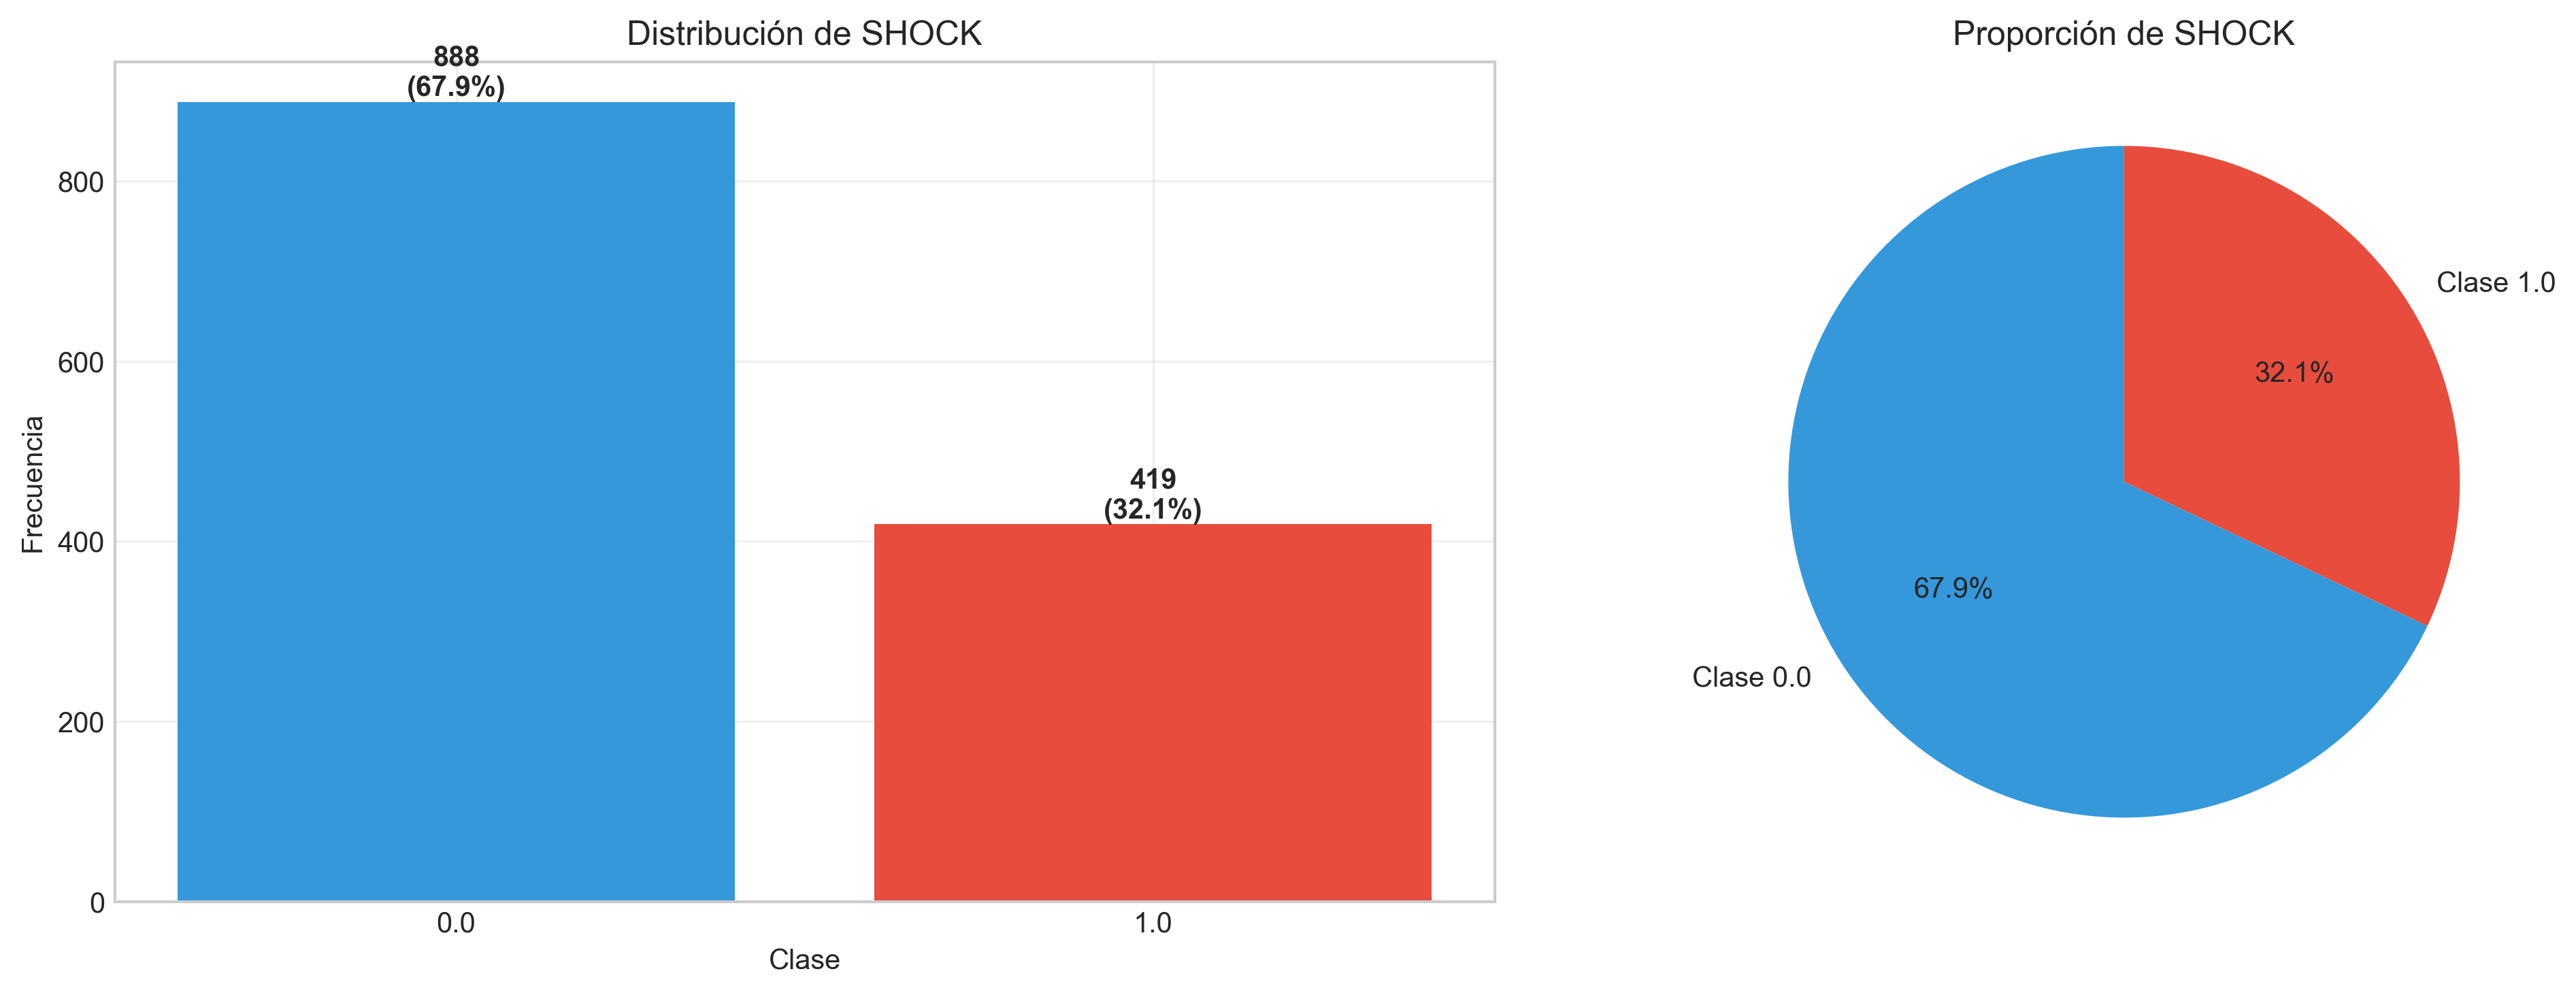
\includegraphics[width=\textwidth]{images/image002.png}
\caption{Variable objetivo - Shock}
\end{figure}

\subsubsection{Variables continuas}

Proseguimos con el análisis de Edad y HB\_PREQX. Lo que vemos son las distribuciones agrupadas por VO, donde las barras de color rosa corresponden a lo casos de shock y las barras de color café corresponden a los casos en los que no hubo shock. Vemos una distribución muy similar a una campana de Gauss para ambas variables, donde la mayoría de los casos se centran en las personas de 60 años para la variable de Edad. De igual forma, la variable HB\_PREQX tiene su mayor peso entre lo niveles 13 y 14. La forma en la que se medirá la relevancia contra la VO para las variables numéricas será con el estadístico de Cohen's d \cite{piasta2010}. Esta es una medida de tamaño del efecto que se utiliza para cuantificar la magnitud de la diferencia entre las medias de dos grupos, expresada en unidades de desviación estándar. Para ejecutarlo correctamente sobre la VO que es binaria, tomaríamos entonces la media de los casos en los que hubo shock y lo restamos con la media de las veces en las que no hubo, esto lo dividimos entre la desviación estándar agrupada para las medias de ambos grupos, formulando lo siguiente:

$$d = \frac{\bar{X}_{shock} - \bar{X}_{no\,shock}}{S_{pooled}}$$

A partir del coeficiente, se ha introducido una serie de rangos de interpretación formulados por el mismo autor del estadístico, los cuales son:

\begin{table}[H]
\centering
\caption{Interpretación del coeficiente de Cohen's d}
\begin{tabular}{|c|c|l|}
\hline
\textbf{Cota inferior (no inclusiva)} & \textbf{Cota superior (inclusiva)} & \textbf{Interpretación} \\ \hline
0 & 0.05 & Efecto muy pequeño \\ \hline
0.05 & 0.15 & Efecto pequeño \\ \hline
0.15 & 0.25 & Efecto mediano \\ \hline
0.25 & $+1$ & Efecto grande \\ \hline
\end{tabular}
\end{table}

Sin embargo, que el coeficiente de Cohens nos diga que es relevante no es suficiente si los datos que tenemos nos indican que realmente no hay suficientes datos para confirmar que es confiable. Para corregir esto usamos el valor P.

El valor P es otro estadístico que nos permite comprobar la hipótesis nula sobre un conjunto de datos \cite{wasserstein2016}. Formalmente se describe como:

Siendo nuestro caso, el que es ``No existe diferencia en las medias poblacionales de la variable numérica entre los dos grupos definidos por la VO.'', cada una de estas hipótesis siendo evaluada a un nivel de confianza de 0.05 para la aceptación de la nula. Así obteniendo tanto relevancia con la VO como confianza sobre la característica.

Con respecto a la descripción estadística de las variables numéricas, encontramos los siguientes datos:

\textbf{Edad:}
\begin{itemize}
    \item Promedio sin shock: 53.71 años
    \item Promedio con shock: 59.57 años
    \item Desviación estándar sin shock: 20.46 años
    \item Desviación estándar con shock: 18.79 años
    \item Mínimo: 1 año
    \item Máximo: 95 años
    \item Cohens-d: 0.294. Medianamente relevante.
    \item P\_value: 3.94E-07. Confiable.
\end{itemize}

\textbf{HB\_PREQX:}
\begin{itemize}
    \item Promedio: 12.926 g/dL
    \item Desviación estándar: 2.023 g/dL
    \item Mínimo: 5 g/dL
    \item Máximo: 19.0 g/dL
    \item Cohens-d: -0.0670. Nada relevante por sí mismo.
    \item P\_value: 0.262. Se rechaza la nula y se acepta que la cantidad de datos de la hemoglobina prequirúrgica por sí sola no es una característica que sea relevante para el entrenamiento.
\end{itemize}

\begin{figure}[H]
\centering
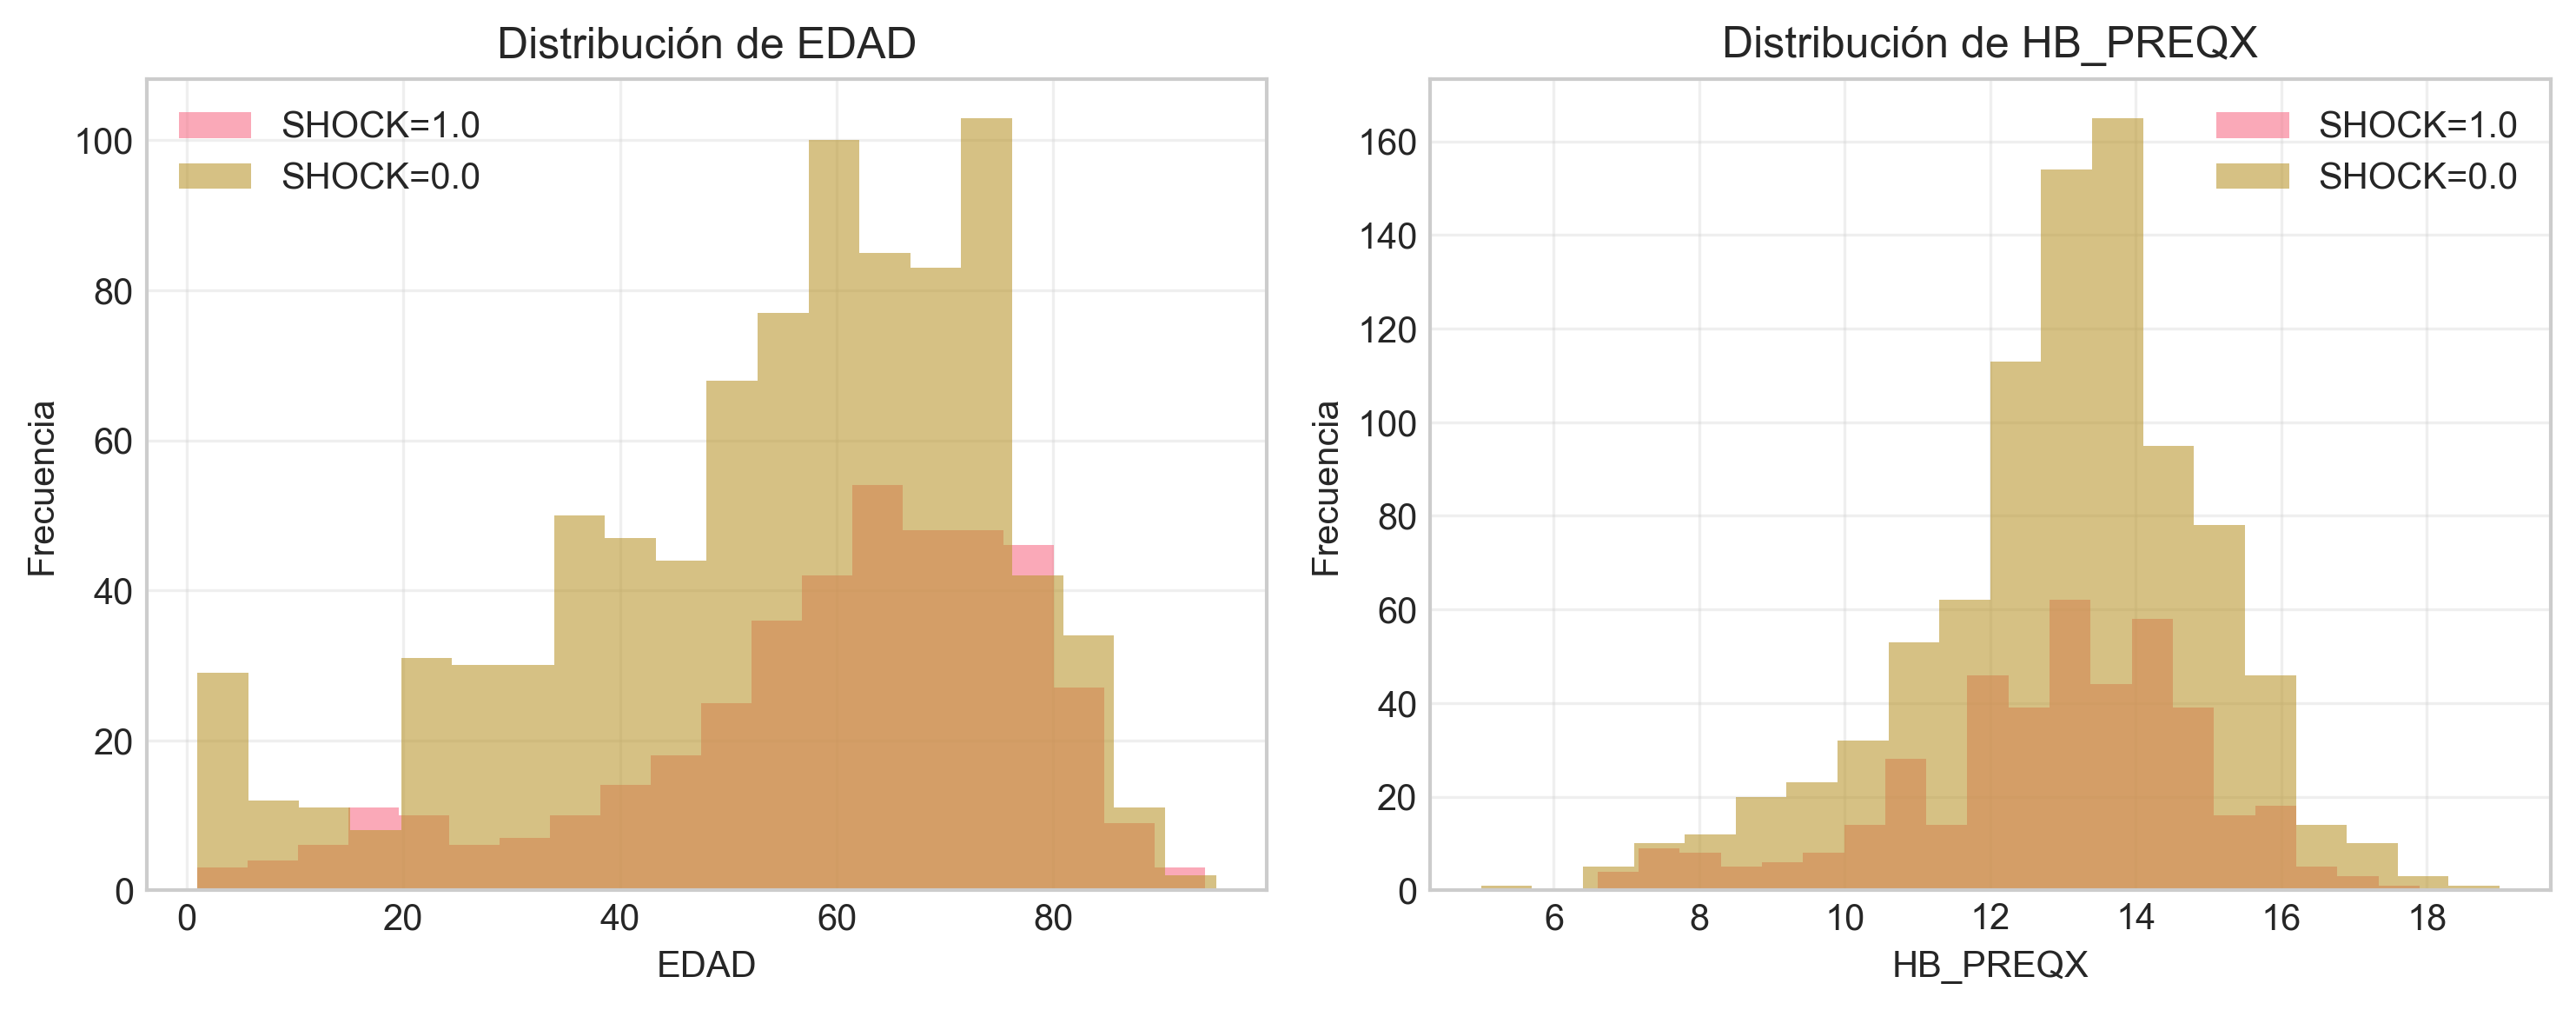
\includegraphics[width=\textwidth]{images/image007.png}
\caption{Interpretación de Cohen's d}
\end{figure}

\subsubsection{Variables booleanas}

La composición del resto del dataset eran datos categóricos booleanos, de estos solo se obtuvo su frecuencia y su relación con la VO. En el proceso describimos cada una de forma general, luego mostraremos nuestro procedimiento para descartar su influencia sobre la VO.

\textbf{GENERO:} Esta variable indica que hay una desproporción en los datos de hombres y mujeres en dataset, ya que vemos que los hombres (1) representan aproximadamente el 32\% del dataset, mientras que las mujeres ocupan aproximadamente el 68\% de este. Concluimos también que el shock afecta de igual forma tanto a hombres en la misma proporción.

\begin{figure}[H]
\centering
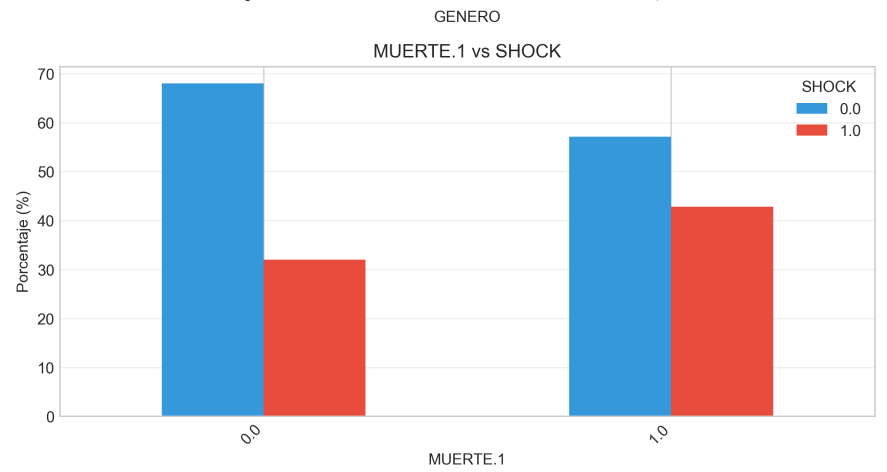
\includegraphics[width=\textwidth]{images/image010.png}
\caption{GENERO: Distribución por género}
\end{figure}

\textbf{ACT\_FISICA\_METS:} Se muestra una proporción similar al género en la actividad física, con un leve decremento cuando hay presencia de shock. Concluimos que el shock afecta en la misma medida a las personas que hacen deporte como a las que no.

\begin{figure}[H]
\centering
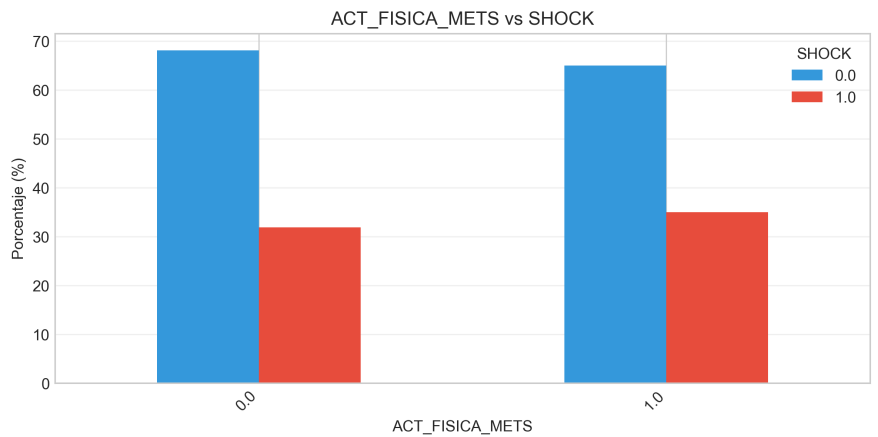
\includegraphics[width=\textwidth]{images/image009.png}
\caption{ACT\_FISICA\_METS: Actividad física}
\end{figure}

\textbf{Muerte:} Esta variable es postoperatoria es inservible cuando se trata de la predicción temprana del shock hipovolémico, por lo que no ha fue tomada en cuenta para el desarrollo temprano del modelo de IA. Sin embargo, esta variable será usada en posteriores análisis para la búsqueda de los mejores selectores. Vemos de igual modo que con respecto a la VO, que no todos los que murieron estuvieron relacionados con el shock.

\begin{figure}[H]
\centering
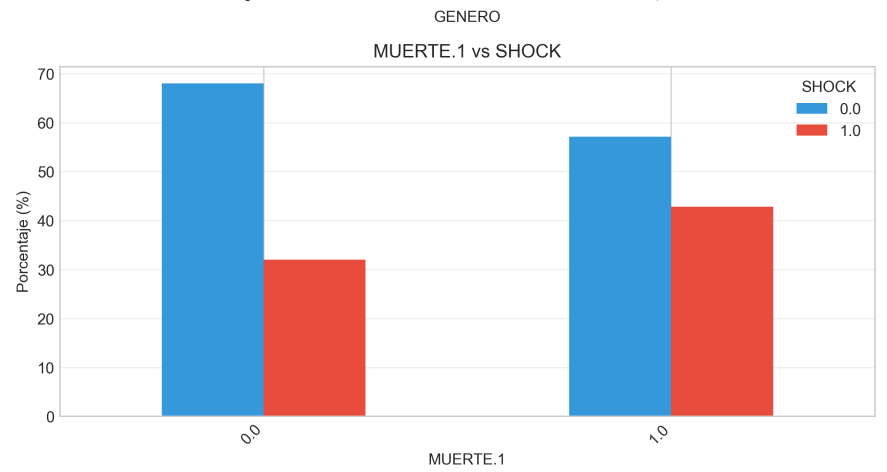
\includegraphics[width=\textwidth]{images/image010.png}
\caption{Muerte: Variable postoperatoria}
\end{figure}

\textbf{HIPERTENSION:} Con respecto al shock, la gráfica muestra que no hay diferencia entre las poblaciones que sufren o no hipertensión.

\begin{figure}[H]
\centering
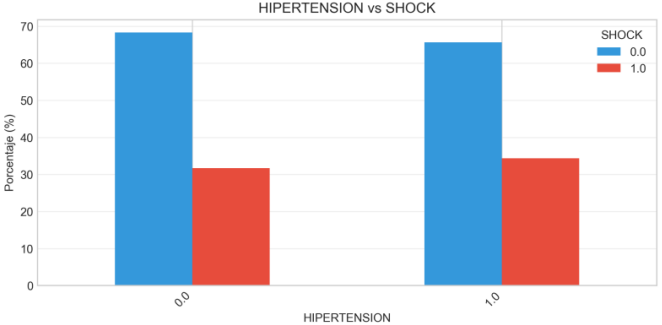
\includegraphics[width=\textwidth]{images/image011.png}
\caption{HIPERTENSION}
\end{figure}

\textbf{DIABETES:} En esta gráfica vemos que tampoco hay una mayor influencia sobre la VO.

\begin{figure}[H]
\centering
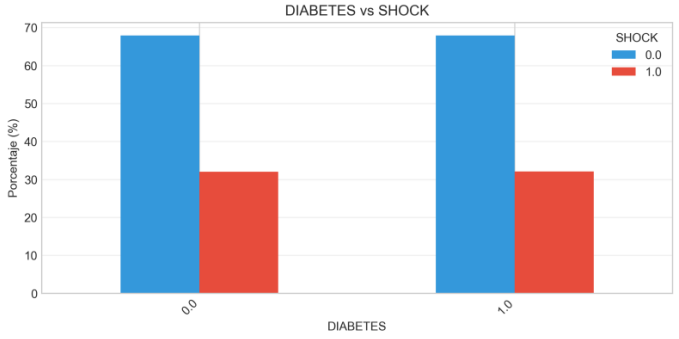
\includegraphics[width=\textwidth]{images/image012.png}
\caption{DIABETES}
\end{figure}

\textbf{ENFERMEDAD\_CORONARIA:} En este caso vemos una mayor influencia sobre la VO cuando se presenta esta comorbilidad, por lo que concluimos que podría ser un factor clave para el entrenamiento o las agregaciones.

\begin{figure}[H]
\centering
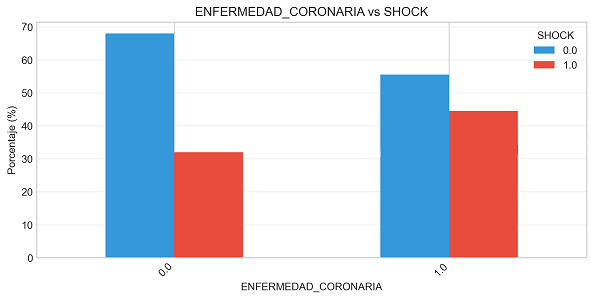
\includegraphics[width=\textwidth]{images/image013.png}
\caption{ENFERMEDAD\_CORONARIA}
\end{figure}

\textbf{FALLA\_CARDIACA:} Esta característica fue tratada como una que se ve afectada por el entorno controlado de los hospitales. Según los expertos de FVL este comportamiento resulta de que las personas con esta complicación son altamente monitoreadas, por lo que son menos propensas a sufrir un shock hipovolémico. Concluimos que la presencia de esta comorbilidad no influye en la VO.

\begin{figure}[H]
\centering
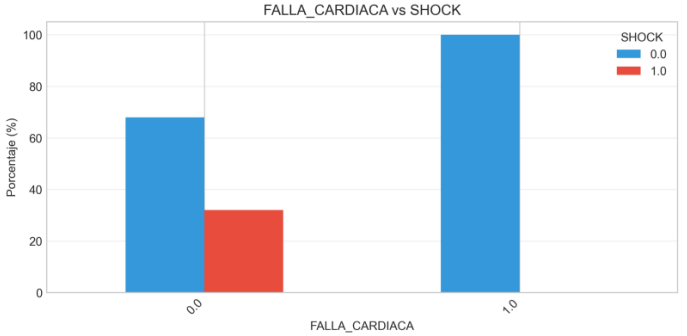
\includegraphics[width=\textwidth]{images/image014.png}
\caption{FALLA\_CARDIACA}
\end{figure}

\textbf{HIPOTIROIDISMO:} Vemos que no tiene mayor influencia en la VO.

\begin{figure}[H]
\centering
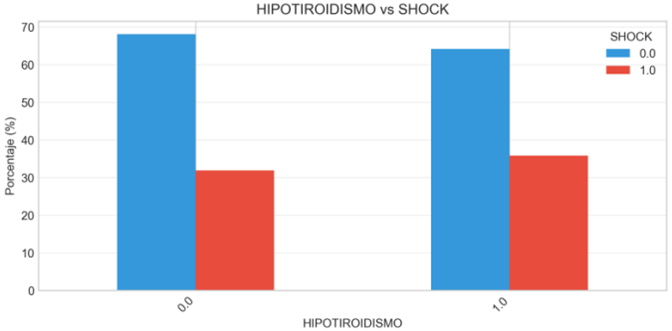
\includegraphics[width=\textwidth]{images/image015.png}
\caption{HIPOTIROIDISMO}
\end{figure}

\textbf{ERC:} Con esta variable podemos concluir que aquellas personas que presentan esta enfermedad son menos propensas a sufrir un shock hipovolémico, según los expertos de FVL tiene la misma explicación que con la falla cardiaca y el alto seguimiento del riesgo con las personas que presentan esta comorbilidad.

\begin{figure}[H]
\centering
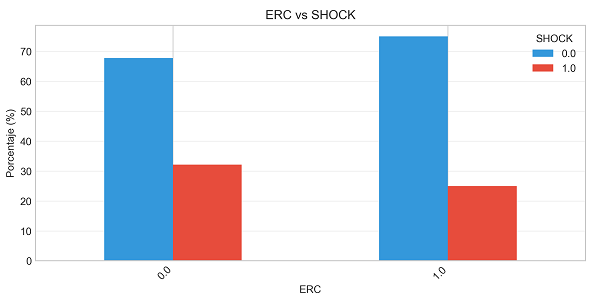
\includegraphics[width=\textwidth]{images/image016.png}
\caption{ERC}
\end{figure}

\textbf{OBESIDAD:} Vemos que la obesidad no influye de forma notoria sobre la VO.

\begin{figure}[H]
\centering
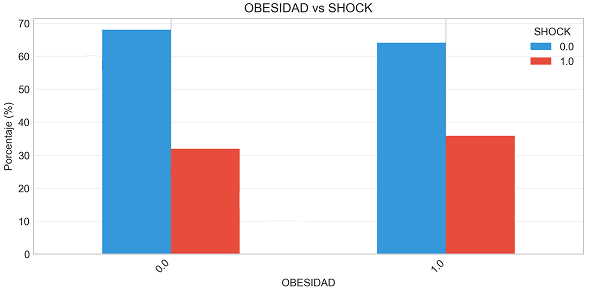
\includegraphics[width=\textwidth]{images/image017.png}
\caption{OBESIDAD}
\end{figure}

\textbf{HIPERTENSION\_PULMONAR:} En este caso, vemos que el poseer o no esta complicación afecta en gran medida el riesgo de shock.

\begin{figure}[H]
\centering
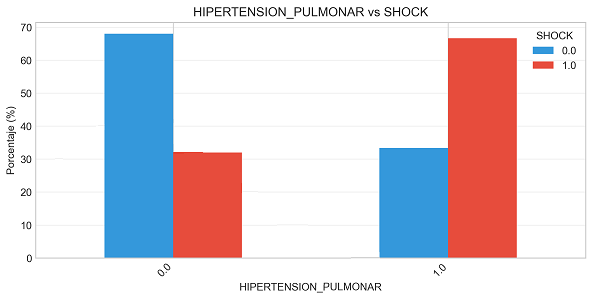
\includegraphics[width=\textwidth]{images/image018.png}
\caption{HIPERTENSION\_PULMONAR}
\end{figure}

\textbf{EPOC:} Aquí vemos que el poseer o no esta enfermedad no influye directamente en la VO.

\begin{figure}[H]
\centering
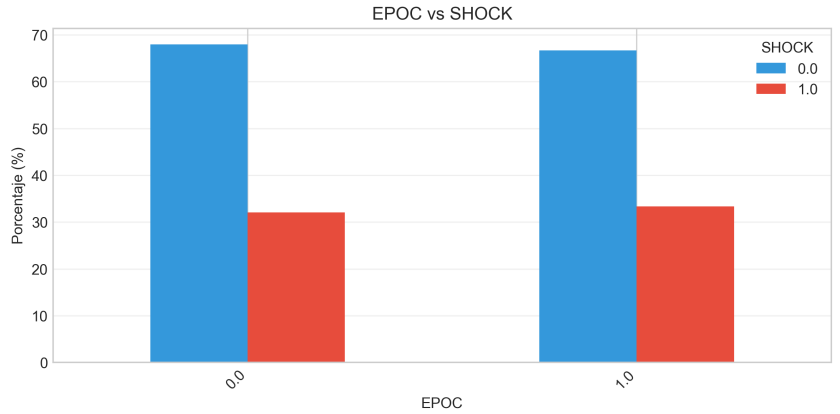
\includegraphics[width=\textwidth]{images/image019.png}
\caption{EPOC}
\end{figure}

\textbf{ASMA:} Vemos que no tiene una mayor incidencia sobre la VO.

\begin{figure}[H]
\centering
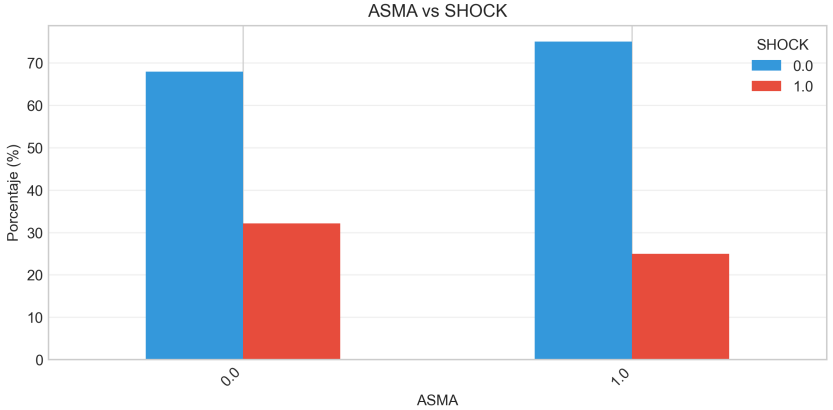
\includegraphics[width=\textwidth]{images/image020.png}
\caption{ASMA}
\end{figure}

\textbf{ENF\_CEREBROVASCULAR:} Vemos que no tiene mayor influencia sobre la VO.

\begin{figure}[H]
\centering
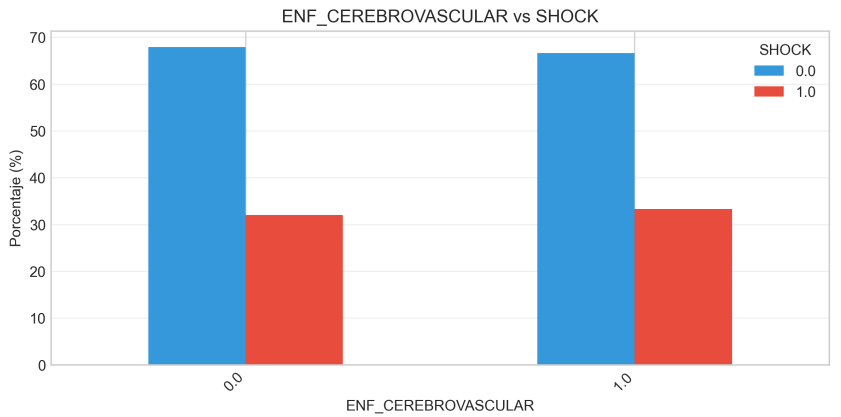
\includegraphics[width=\textwidth]{images/image021.png}
\caption{ENF\_CEREBROVASCULAR}
\end{figure}

\subsection{Discriminación inicial de la relevancia de las características sobre la VO}

Para poder tener una comprensión más detallada de que comorbilidades influían realmente sobre la VO usamos la matriz de coeficientes de Cramér's V \cite{allen2017}. Esta es una medida de asociación entre dos variables nominales que proporciona un valor entre 0 y 1 (inclusivo), donde 0 indica ausencia de asociación y 1 indica asociación perfecta. Este coeficiente se basa en la estadística de chi-cuadrado de Pearson y fue desarrollado por el estadístico sueco Harald Cramér.

La matriz de coeficientes de Cramér's V extiende este concepto calculando el coeficiente de Cramér's V para cada par de variables categóricas en un dataset, creando así una lista de correlación específica para variables categóricas, concepto ideal para el análisis de las comorbilidades booleanas. Al hacer la aplicación sobre el dataset se obtuvo la siguiente figura.

\begin{figure}[H]
\centering
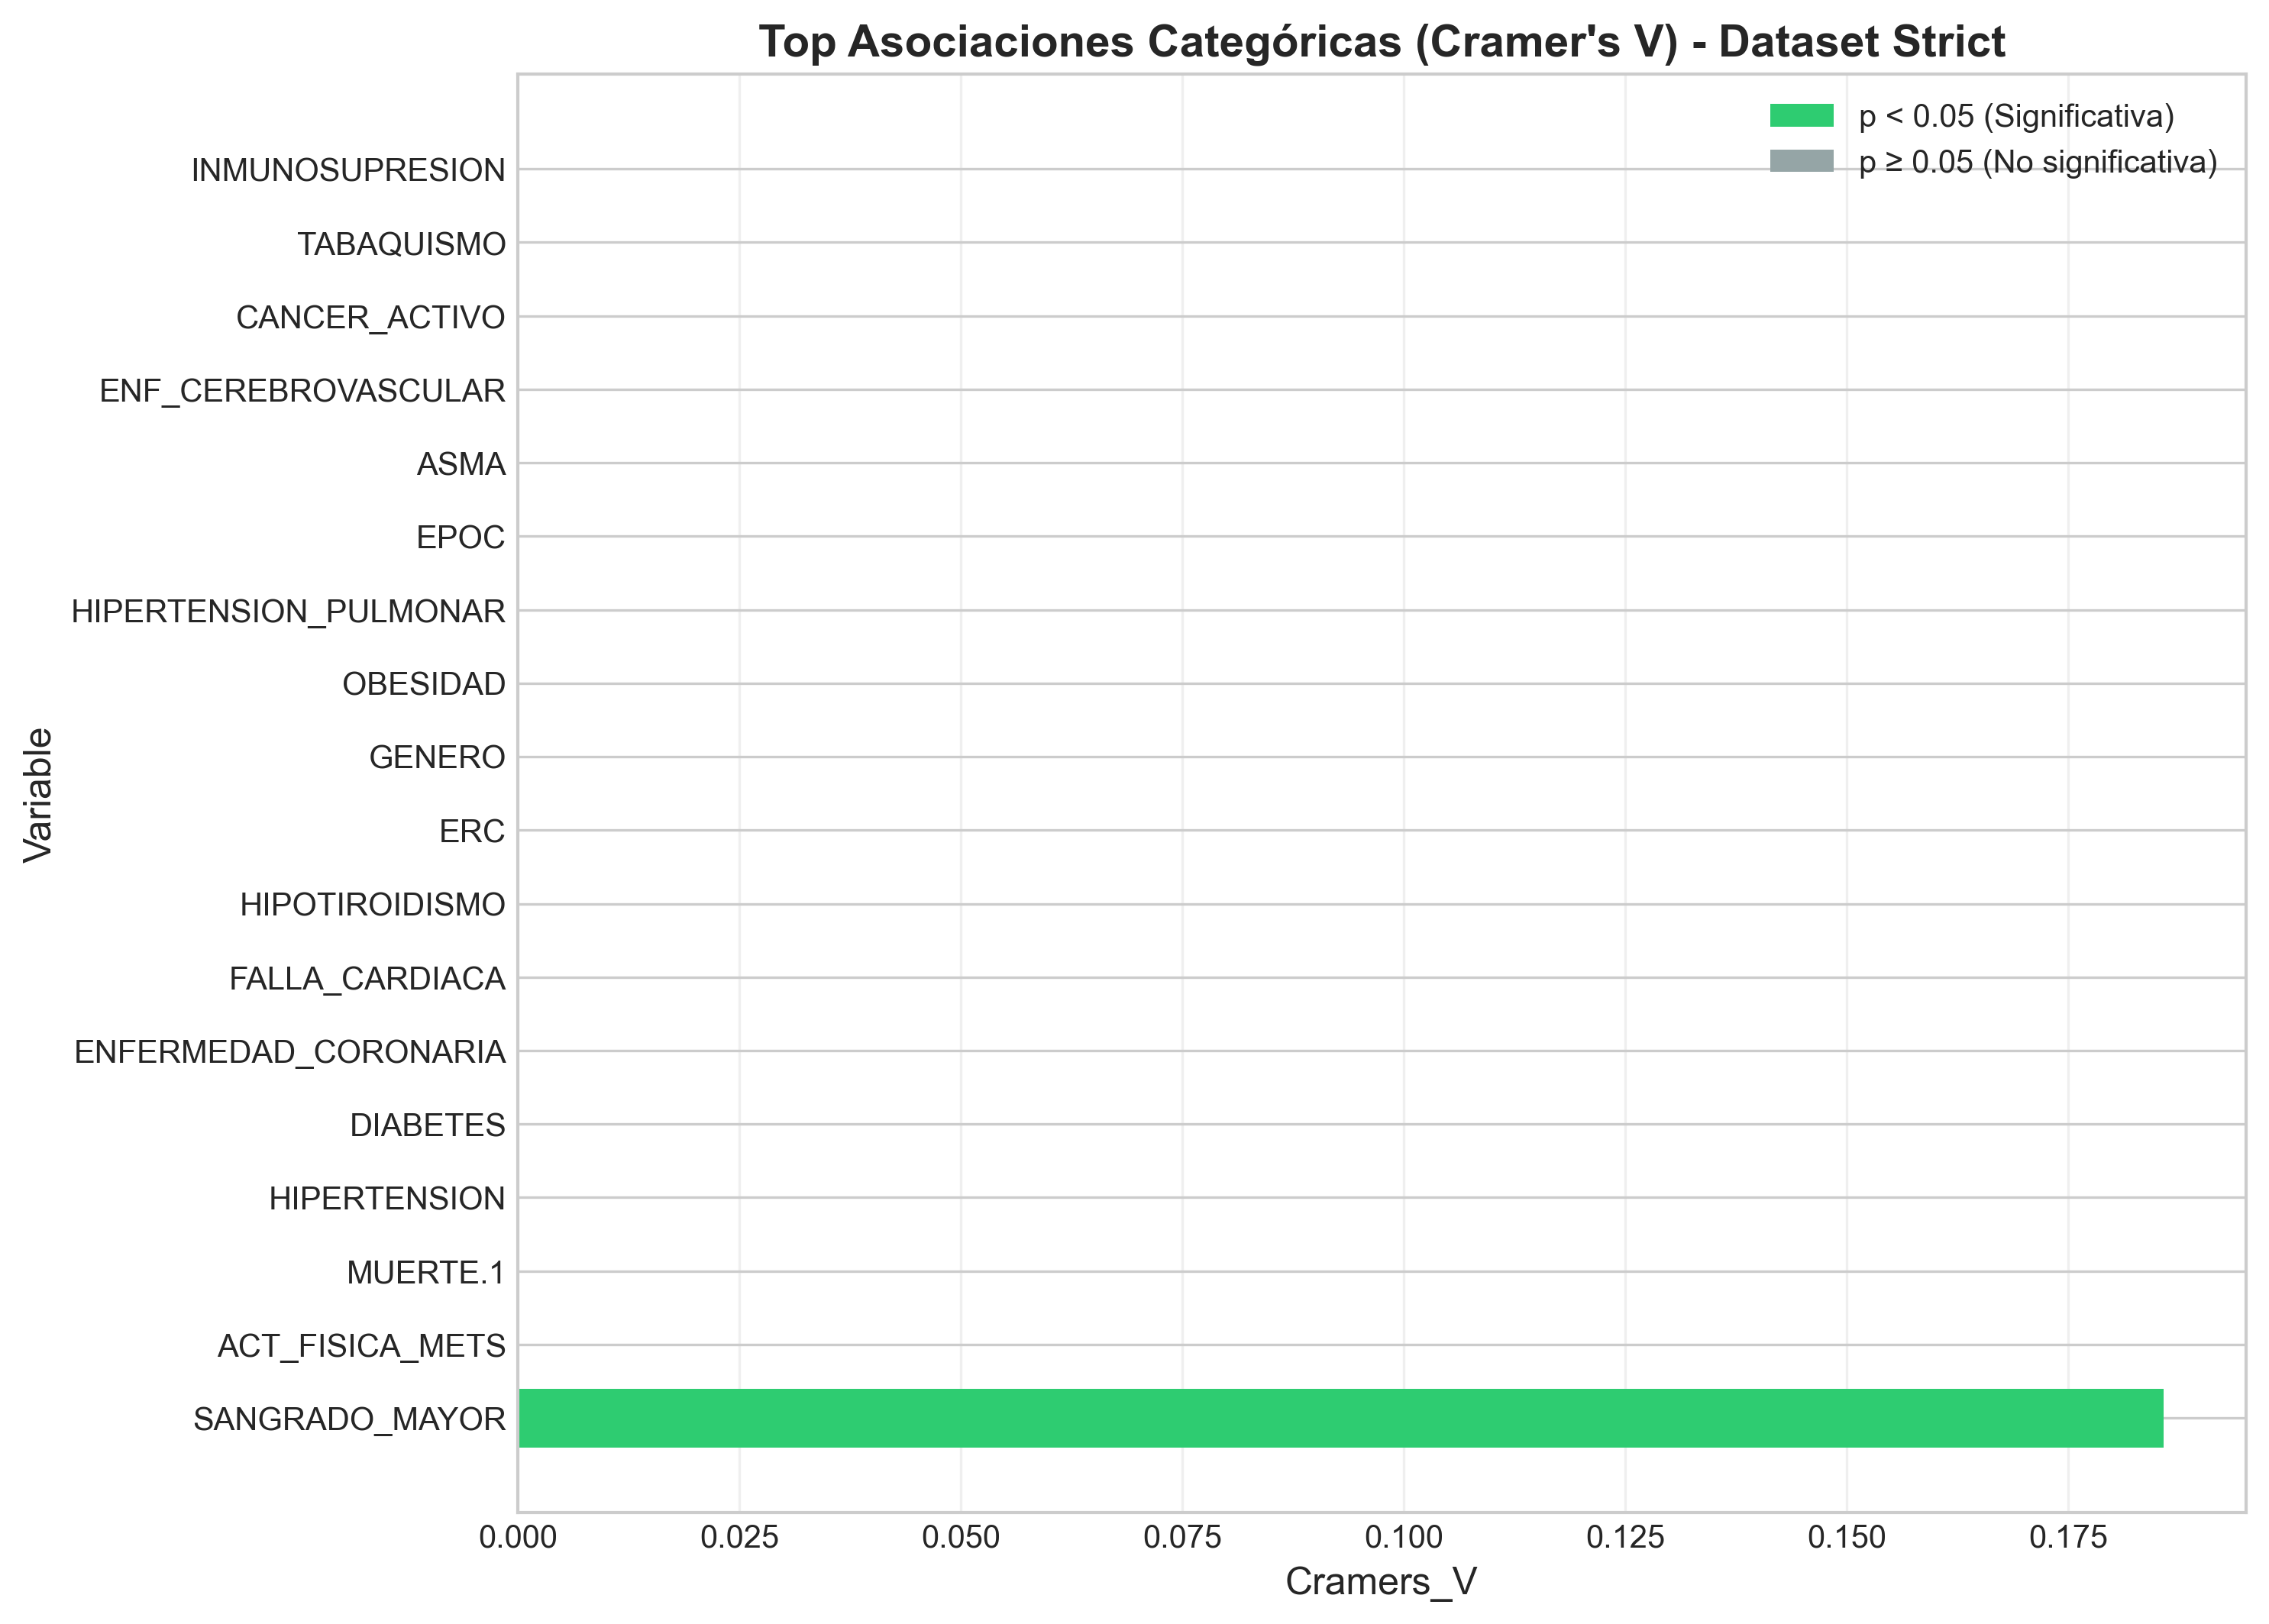
\includegraphics[width=\textwidth]{images/image022.png}
\caption{Matriz de Cramér's V}
\end{figure}

Según lo mencionado previamente, esta figura indica que la única que es capaz de superar el umbral de significancia con el estadístico de Cramér's V es SANGRADO\_MAYOR. Esto significa que por sí solas, el resto de las características entregadas en el dataset son irrelevantes para la predicción del shock hemorrágico. Para demostrar esta incapacidad de predicción, nos dispusimos a hacer un entrenamiento preliminar que considerara el dataset virgen, sin ningún tipo de asociación o agregación.

\subsection{Modelaje preliminar}

Se decidió ver el rendimiento inicial del dataset para comprender en mejor medida su estado. El entrenamiento preliminar se realizó en forma de un pipeline robusto que nos permitiera hacer varias ejecuciones de manera sencilla sobre el conjunto de datos.

\textbf{Consideraciones del pipeline:}

\begin{itemize}
    \item Prevención del Data leakage: Se evitó la variable muerte ya que era post operativa.
    \item Manejo del desbalance de la VO
    \item Reproducibilidad
    \item Se creó una variable HB\_normal que indica si los niveles de hemoglobina están dentro de los rasgos clínicamente aceptables según edad y sexo, se usaron estándares reconocidos por la secretaría de seguridad de los Estados Unidos.
    \item Los datos se dividieron en dos conjuntos iniciales, train y test, con un 80\% y un 20\% respectivamente, con estratificación en la VO.
    \item Se realizó una validación cruzada con 5 folds estratificados durante el entrenamiento. Adicionalmente se instauró una semilla fija, 42 en nuestro caso, para la reproducibilidad.
    \item Como ya se ha mencionado previamente, no hay variables en nulo ni variables repetidas, sin embargo existían variables como FALLA\_CARDIACA y TABAQUISMO, los cuales tenían datos entre 0 y 2 a pesar de que era una variable categórica binaria, según FVL esos datos eran erróneos y debían ser eliminados, se encontraron 17 que se removieron del dataset, dicha eliminación correspondió al 1.28\% de los datos.
    \item El manejo del desbalance se ajustó con el algoritmo de SMOTE, el cual fue aplicado únicamente dentro de los folds de entrenamiento durante la validación cruzada para evitar sobreestimación. De igual forma se usó el método class weight para los modelos que lo aceptaban.
\end{itemize}

\textbf{Modelos evaluados:}

\begin{itemize}
    \item Regresión logística regularizada (Lasso). Ya que fue una de las elecciones de mayor éxito según la literatura.
    \item Random forest. Pues naturalmente se usa para las variables binarias por su naturaleza discreta
    \item XGBoost. Según la literatura también de los modelos con mejor rendimiento.
\end{itemize}

\textbf{Métricas utilizadas:}

\begin{itemize}
    \item Recall: Porcentaje de casos de shock correctamente identificados.
    \item Especifidad: Porcentaje de no shock correctamente identificados.
    \item AUC-ROC: Capacidad discriminativa general.
    \item Precisión: Relevancia de los positivos detectados.
\end{itemize}

\textbf{Ajuste de umbral clínico:}

\begin{itemize}
    \item Criterio principal: Maximizar recall manteniendo especificidad mínima de 60\%.
    \item Mecanismo: Búsqueda de curvas ROC para encontrar el umbral óptimo.
    \item Validación: Intervalos de confianza Bootstrap (con 1000 iteraciones) para el recall final.
\end{itemize}

\textbf{Resultados del modelaje experimental:} Los resultados finales de modelaje entregaron resultados esperados.

\begin{figure}[H]
\centering
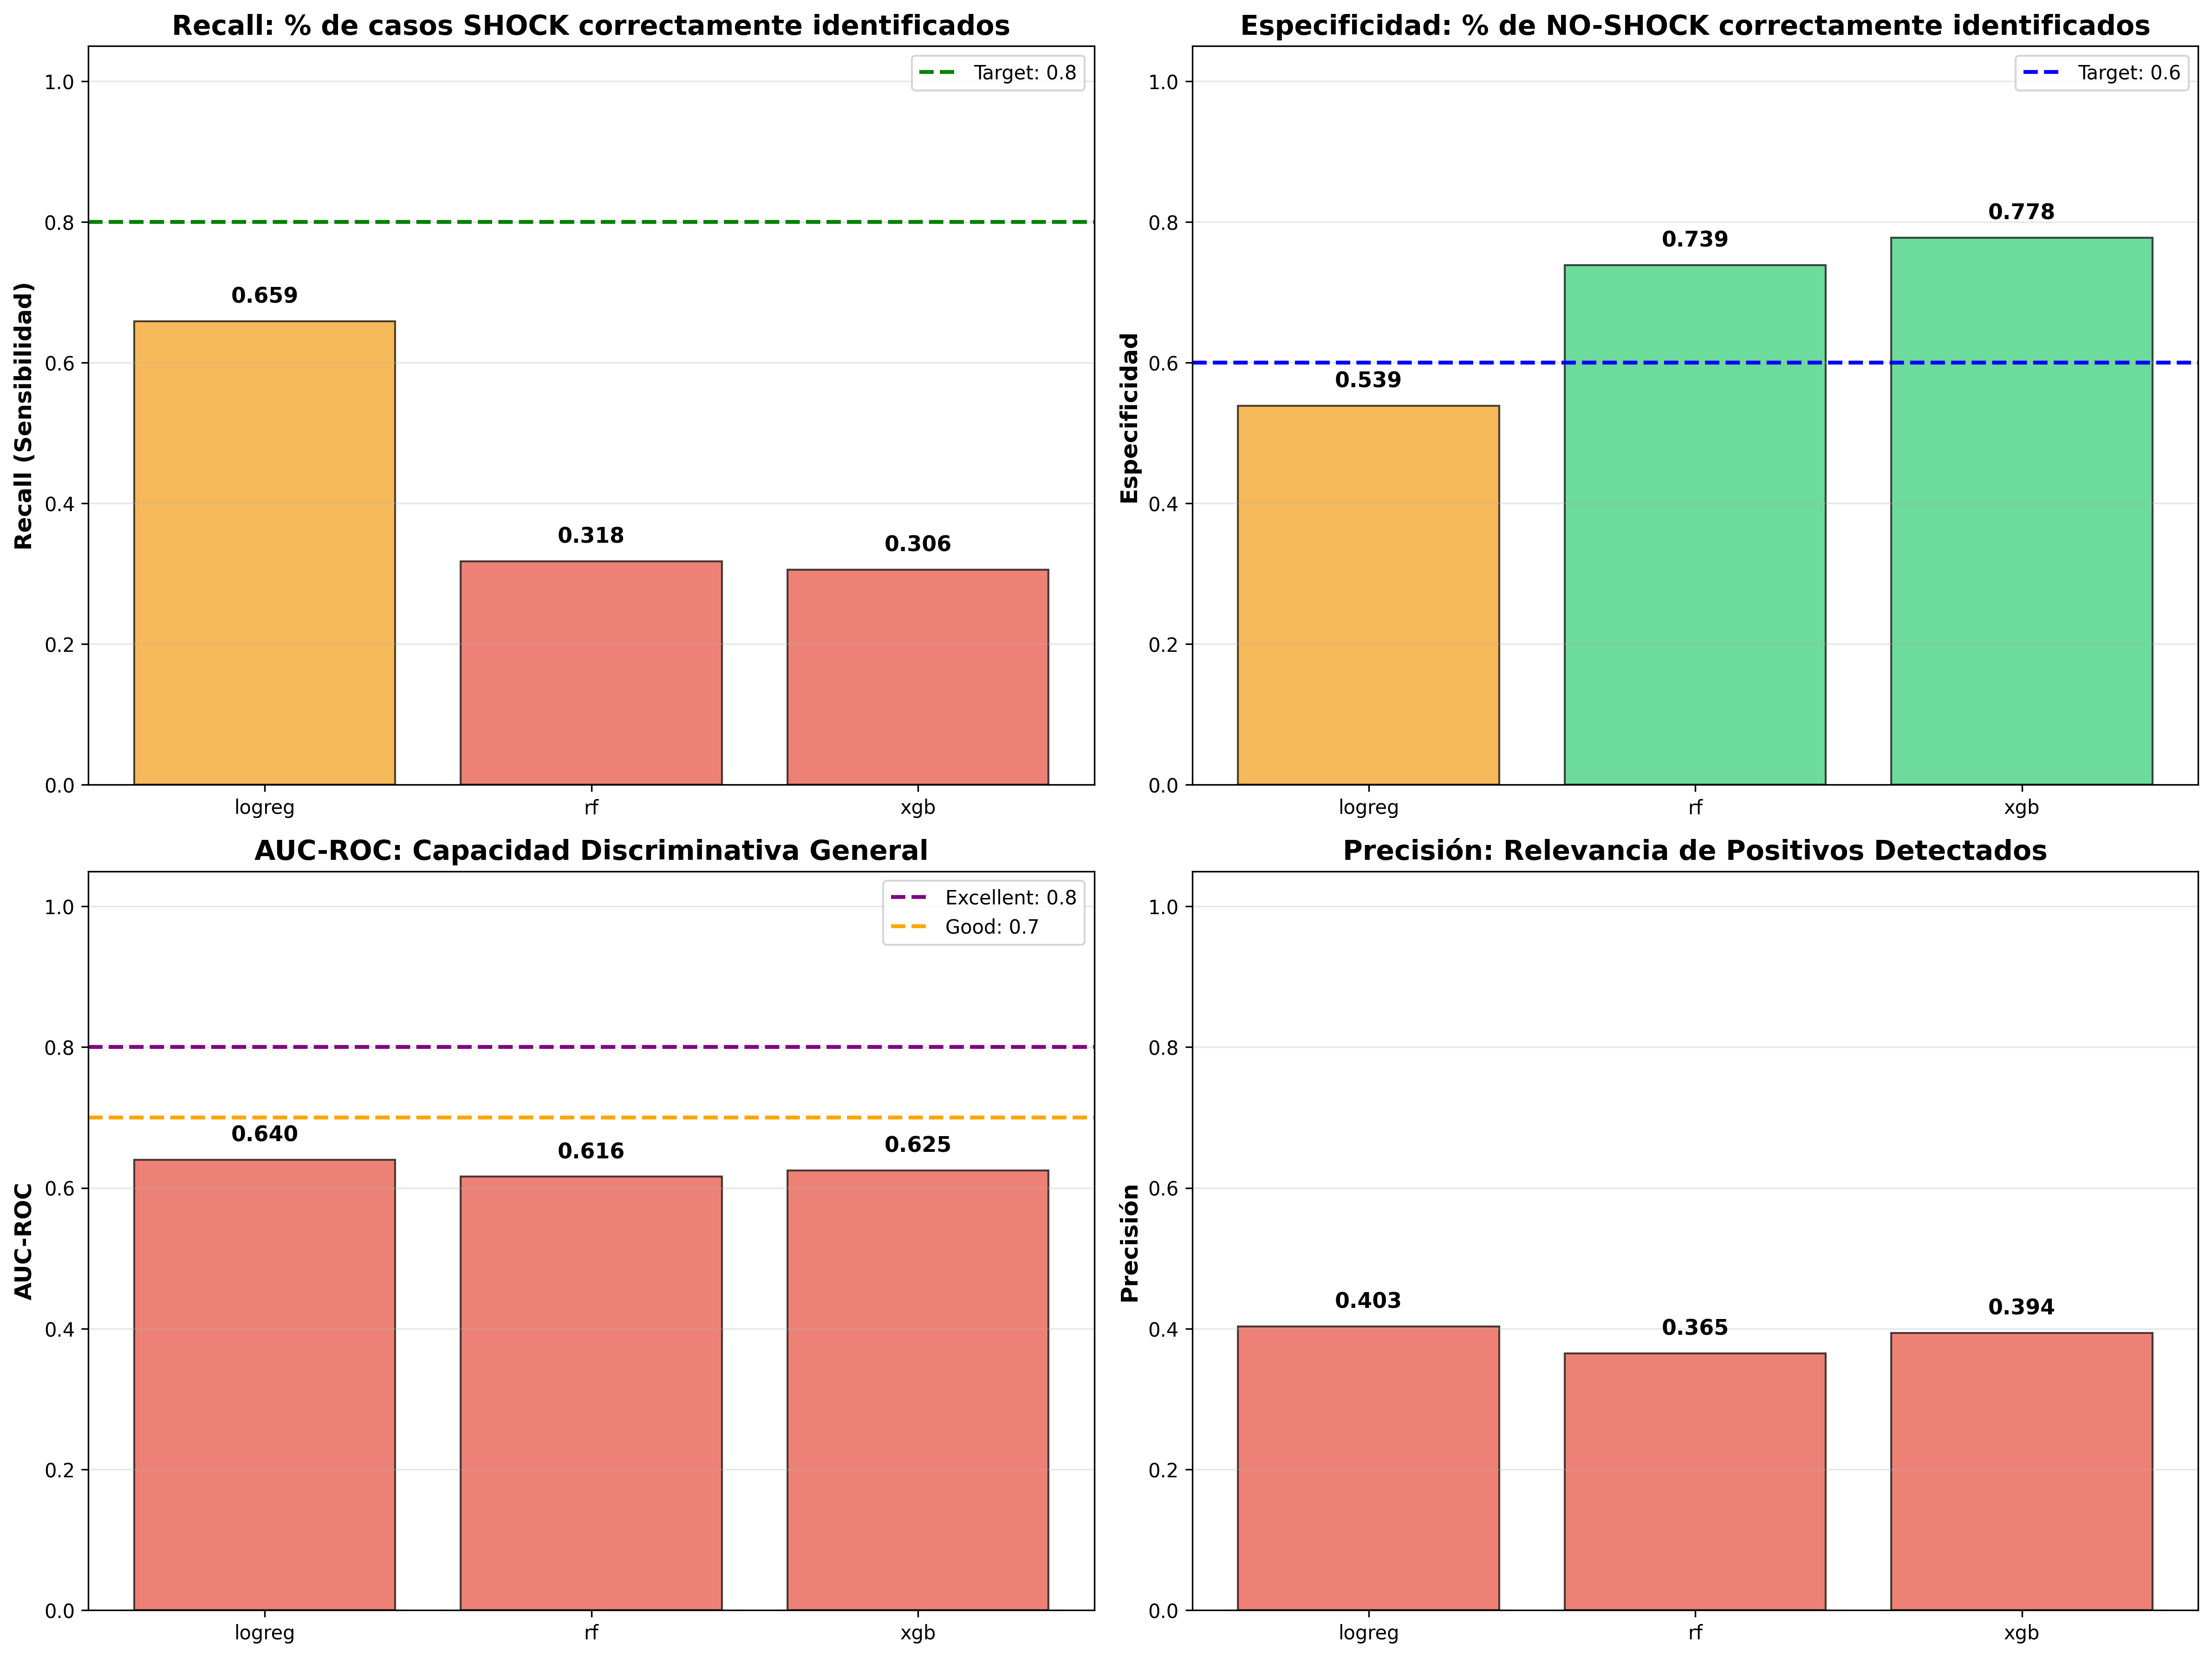
\includegraphics[width=\textwidth]{images/image023.png}
\caption{Resultados del modelaje experimental}
\end{figure}

En las gráficas podemos ver RECALL, AUC-ROC, Especificidad y Precisión. Los resultados muestran que ningún modelo logra hacer una predicción correcta que supere el porcentaje de datos que están presentes dentro del dataset. Nuestro modelo final debe de detectar correctamente los casos de shock por encima de los casos no shock, ya que la presencia de este no detectado puede resultar en la muerte de una persona, es así como nos interesa principalmente que el modelo sea capaz de detectar el shock y que sea capaz de diferenciar correctamente las probabilidades de que una persona pueda o no tener shock. Vemos entonces que el Recall en el mejor de los casos con 0.65 es completamente deficiente para esta tarea, pues es muy cercano del azar. El AUC-ROC se controla de la misma manera siendo 0.64 el mejor modelo. El dataset tiene aproximadamente un 32\% de casos en los que hay presencia de shock, lo que quiere decir los resultados obtenidos por el Recall, en el mejor de los casos, se debe a un sobre ajuste del modelo sobre los datos.

\subsection{Feature engineering}

Dado que la mayoría de los datos por si solos son irrelevantes y que los modelos presentan un sobreajuste sobre los datos, haremos técnicas de feature engineering de forma que podamos extraer más información del dataset con agregaciones, segmentaciones y asociaciones de datos.

\textbf{Variables agregadas:}

\textbf{Agregaciones clínicas}

\textbf{CARGA\_COMORBILIDADES:} Conteo de comorbilidades (0--13). Suma simple de 13 condiciones crónicas, se fundamenta principalmente en la suma de comorbilidades de Charlson, en las que están incluídas:

Hipertensión, diabetes, enfermedad coronaria, falla cardiaca, hipotiroidismo, erc, inmunosupresión, obesidad, hipertensión pulmonar, epoc, asma, enfermedad cerebrovascular y cancer activo.

\textbf{FACTORES\_RIESGO\_SANGRADO:} Interacción clínica (sangrado + tabaquismo).

\textbf{SANGRADO\_X\_CV:} Interacción multiplicativa entre sangrado y riesgo cardiovascular (sangrado + riesgo cardiovascular).

\textbf{Variables agrupadas:}

\textbf{CATEGORIA\_EDAD:} Según Centros para el Control y la Prevención de Enfermedades de Estados Unidos, la edad se puede dividir en ciertas categorías, adicionalmente se agrega la categoría para menores de 18 ya que existen mínimos de 1 año en el dataset y estos son casos posibles que deben ser considerados en el dataset.

\begin{itemize}
    \item 0 -- Pediátrico: edad < 18 años
    \item 1 -- Adulto joven: 18 $\leq$ edad < 45 (etiqueta: 18--44)
    \item 2 -- Adulto medio: 45 $\leq$ edad < 65 (45--64)
    \item 3 -- Adulto mayor: 65 $\leq$ edad < 75 (65--74)
    \item 4 -- Anciano: edad $\geq$ 75
\end{itemize}

\textbf{CATEGORIA\_HB\_PREQX:} Categorización clínica de rangos según la OMS:

\begin{itemize}
    \item 0 -- Normal: HB $\geq$ 12 g/dL
    \item 1 -- Anemia leve: 10.0 $\leq$ HB < 12.0 g/dL (10--11.9)
    \item 2 -- Anemia moderada: 8.0 $\leq$ HB < 10.0 g/dL (8--9.9)
    \item 3 -- Anemia severa: HB < 8.0 g/dL
\end{itemize}

\textbf{Resultados:}

La variable de risk score se encontró que esta es realmente significativa, ya que su valor P es de 4.54e-09 y su coeficiente de Cohens-d es de 0.282.

Con respecto al resto de variables creadas, se realizó de nuevo Cramér's V sobre estas, se encontró que ahora, CATEGORIA\_EDAD, FACTORES\_RIESGO\_SANGRADO\_MAYOR, SANGRADO\_MAYOR y SANGRADO\_X\_CV. Ya que estas ahora si superan el umbral de significancia.

\begin{figure}[H]
\centering
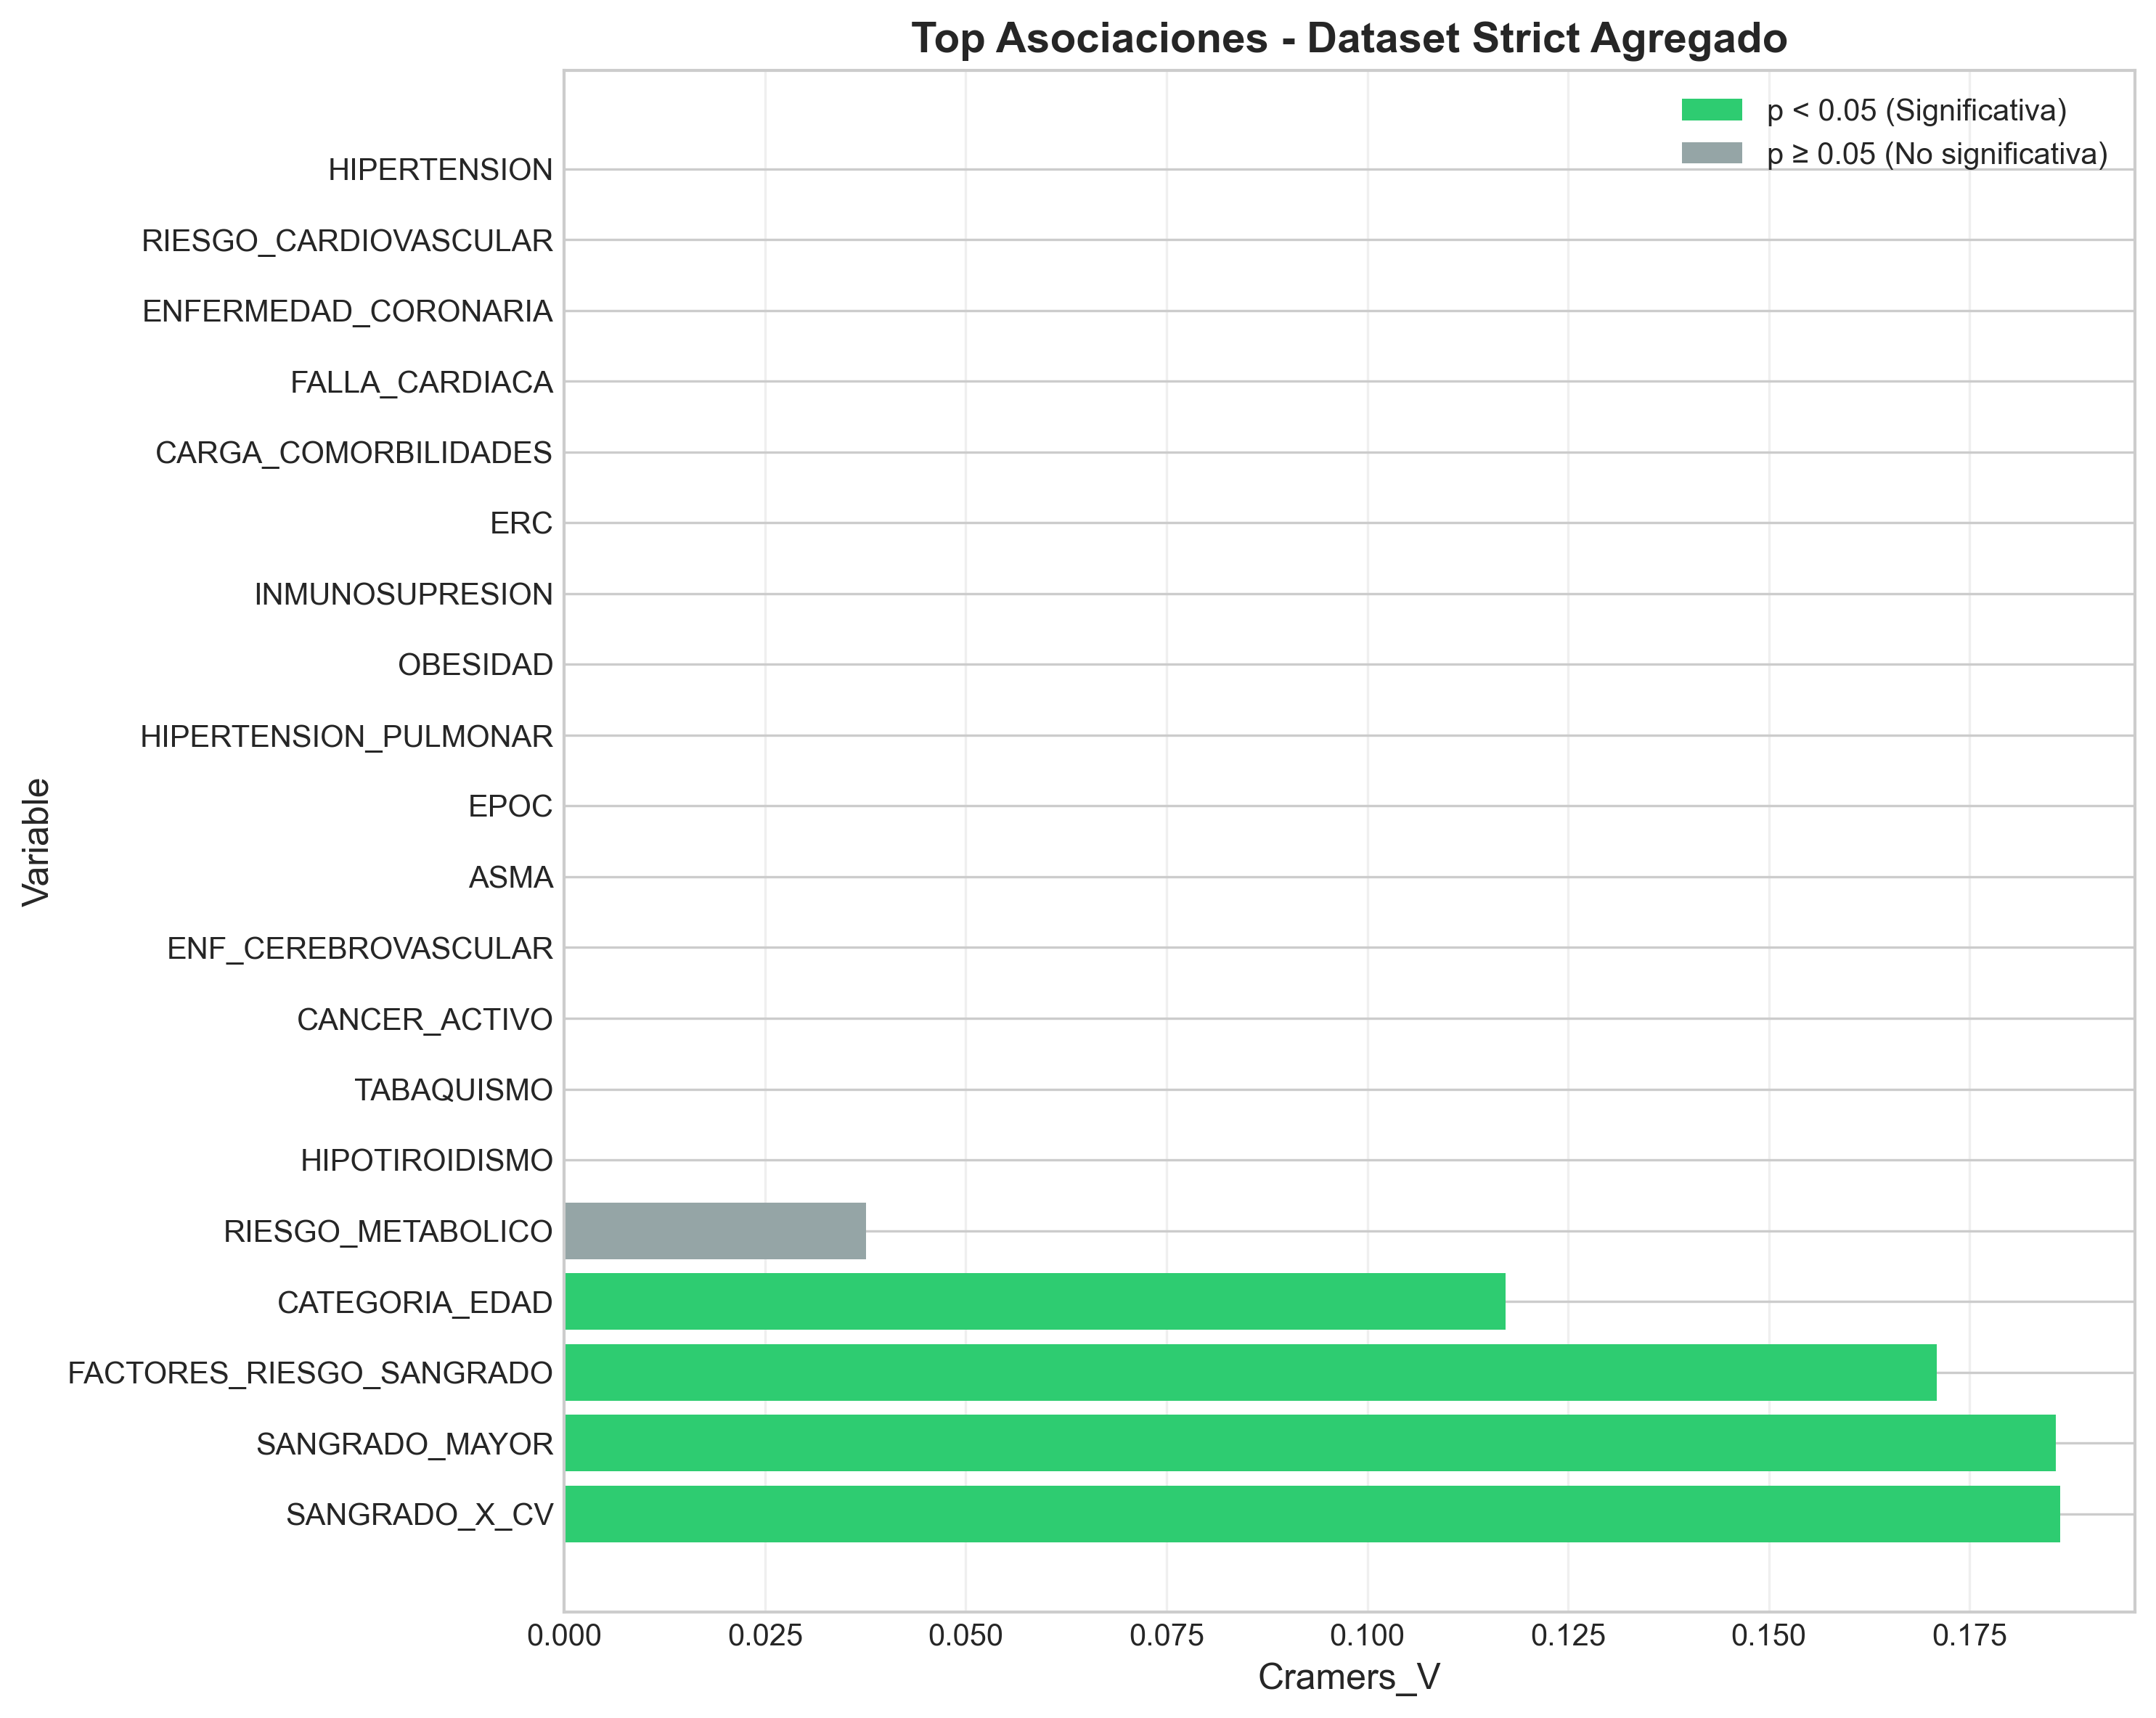
\includegraphics[width=\textwidth]{images/image024.png}
\caption{Matriz de Cramér's V con variables agregadas}
\end{figure}

La creación de nuevas variables por medio de las ya presentes en el dataset genera colinealidades entre variables, lo que puede incurrir en ruido para los modelos en su entrenamiento. Para evitar esto, removeremos las menos significativas en la etapa de entrenamiento para poder tener un contraste real de cuales generan ruido en el modelo y cuales son realmente necesarias para la comprensión del shock.

\subsection{Experimentación y análisis de modelos}

Con el objetivo de identificar la mejor configuración de características y algoritmos para la predicción del shock hemorrágico, se diseñó una serie de experimentos sistemáticos. Cada experimento fue documentado, permitiendo la trazabilidad de los resultados y la comparación rigurosa entre diferentes enfoques. Se realizaron múltiples iteraciones experimentales, cada una explorando distintas combinaciones de ingeniería de características, hiperparámetros y algoritmos de aprendizaje automático.

\textbf{Resumen de experimentos realizados:}

\begin{itemize}
    \item \textbf{Experimento base:} Evaluación inicial con el dataset original conteniendo variables demográficas, clínicas y comorbilidades. Establece la línea base con AUC-ROC de 0.58.
    \item \textbf{Categorización:} Transformación de EDAD y HB\_PREQX en categorías clínicas. No produjo mejoras significativas.
    \item \textbf{Agregaciones:} Creación de variables compuestas (CARGA\_COMORBILIDADES, FACTORES\_RIESGO\_SANGRADO). Sin mejora en rendimiento.
    \item \textbf{Combinación:} Uso conjunto de categorización y agregaciones. Rendimiento similar al base.
    \item \textbf{Ajuste de hiperparámetros:} Búsqueda en grilla para optimizar modelos. Mejoras marginales.
    \item \textbf{Nuevos modelos:} Incorporación de KNN y LightGBM. AUC-ROC inicial de 0.508.
    \item \textbf{Reglas de asociación:} Selección de características basada en patrones frecuentes. Rendimiento inferior.
    \item \textbf{Inclusión de SANGRADO\_MAYOR:} Tras validación con especialistas, se habilita esta variable. AUC-ROC mejora a 0.653.
    \item \textbf{Modelos interpretables:} Evaluación de Decision Tree y Naive Bayes para explicabilidad clínica.
\end{itemize}

\subsubsection{Configuración experimental}

Todos los experimentos compartieron la siguiente configuración:

\begin{itemize}
    \item División de datos: 80\% entrenamiento, 20\% prueba con estratificación.
    \item Validación cruzada estratificada con 5 folds (posteriormente 10 folds en versiones avanzadas).
    \item Semilla fija (42) para reproducibilidad.
    \item Manejo del desbalance mediante SMOTE y pesos de clase.
    \item Métricas principales: Recall, Precisión, Especificidad, F1-Score y AUC-ROC.
\end{itemize}

\subsubsection{Experimento base: Dataset sin procesamiento adicional}

El primer experimento estableció la línea base utilizando únicamente las características originales del dataset, sin variables derivadas ni categorización. Se evaluaron tres algoritmos: Regresión Logística, Random Forest y Gradient Boosting.

\begin{table}[H]
\centering
\caption{Resultados del experimento base en conjunto de prueba}
\label{tab:exp-base}
\begin{tabular}{|l|c|c|c|c|c|}
\hline
\textbf{Modelo} & \textbf{Recall} & \textbf{Precisión} & \textbf{Especificidad} & \textbf{F1-Score} & \textbf{AUC-ROC} \\ \hline
Regresión Logística & 0.929 & 0.322 & 0.079 & 0.479 & 0.580 \\ \hline
Random Forest & 0.714 & 0.335 & 0.331 & 0.456 & 0.532 \\ \hline
Gradient Boosting & 0.238 & 0.345 & 0.787 & 0.282 & 0.532 \\ \hline
\end{tabular}
\end{table}

Los resultados confirmaron la hipótesis inicial: utilizando solo las características originales, los modelos presentan un rendimiento limitado. La Regresión Logística alcanzó el mayor recall (0.929), pero con una especificidad extremadamente baja (0.079), lo que indica que el modelo no está ``aprendiendo'' patrones discriminativos, sino que simplemente clasifica a casi todos los pacientes como casos positivos. Este comportamiento es un síntoma típico del desbalance de clases y no debe interpretarse como un buen rendimiento. El AUC-ROC cercano a 0.5 en todos los modelos confirma una capacidad discriminativa apenas superior al azar.

\begin{figure}[H]
\centering
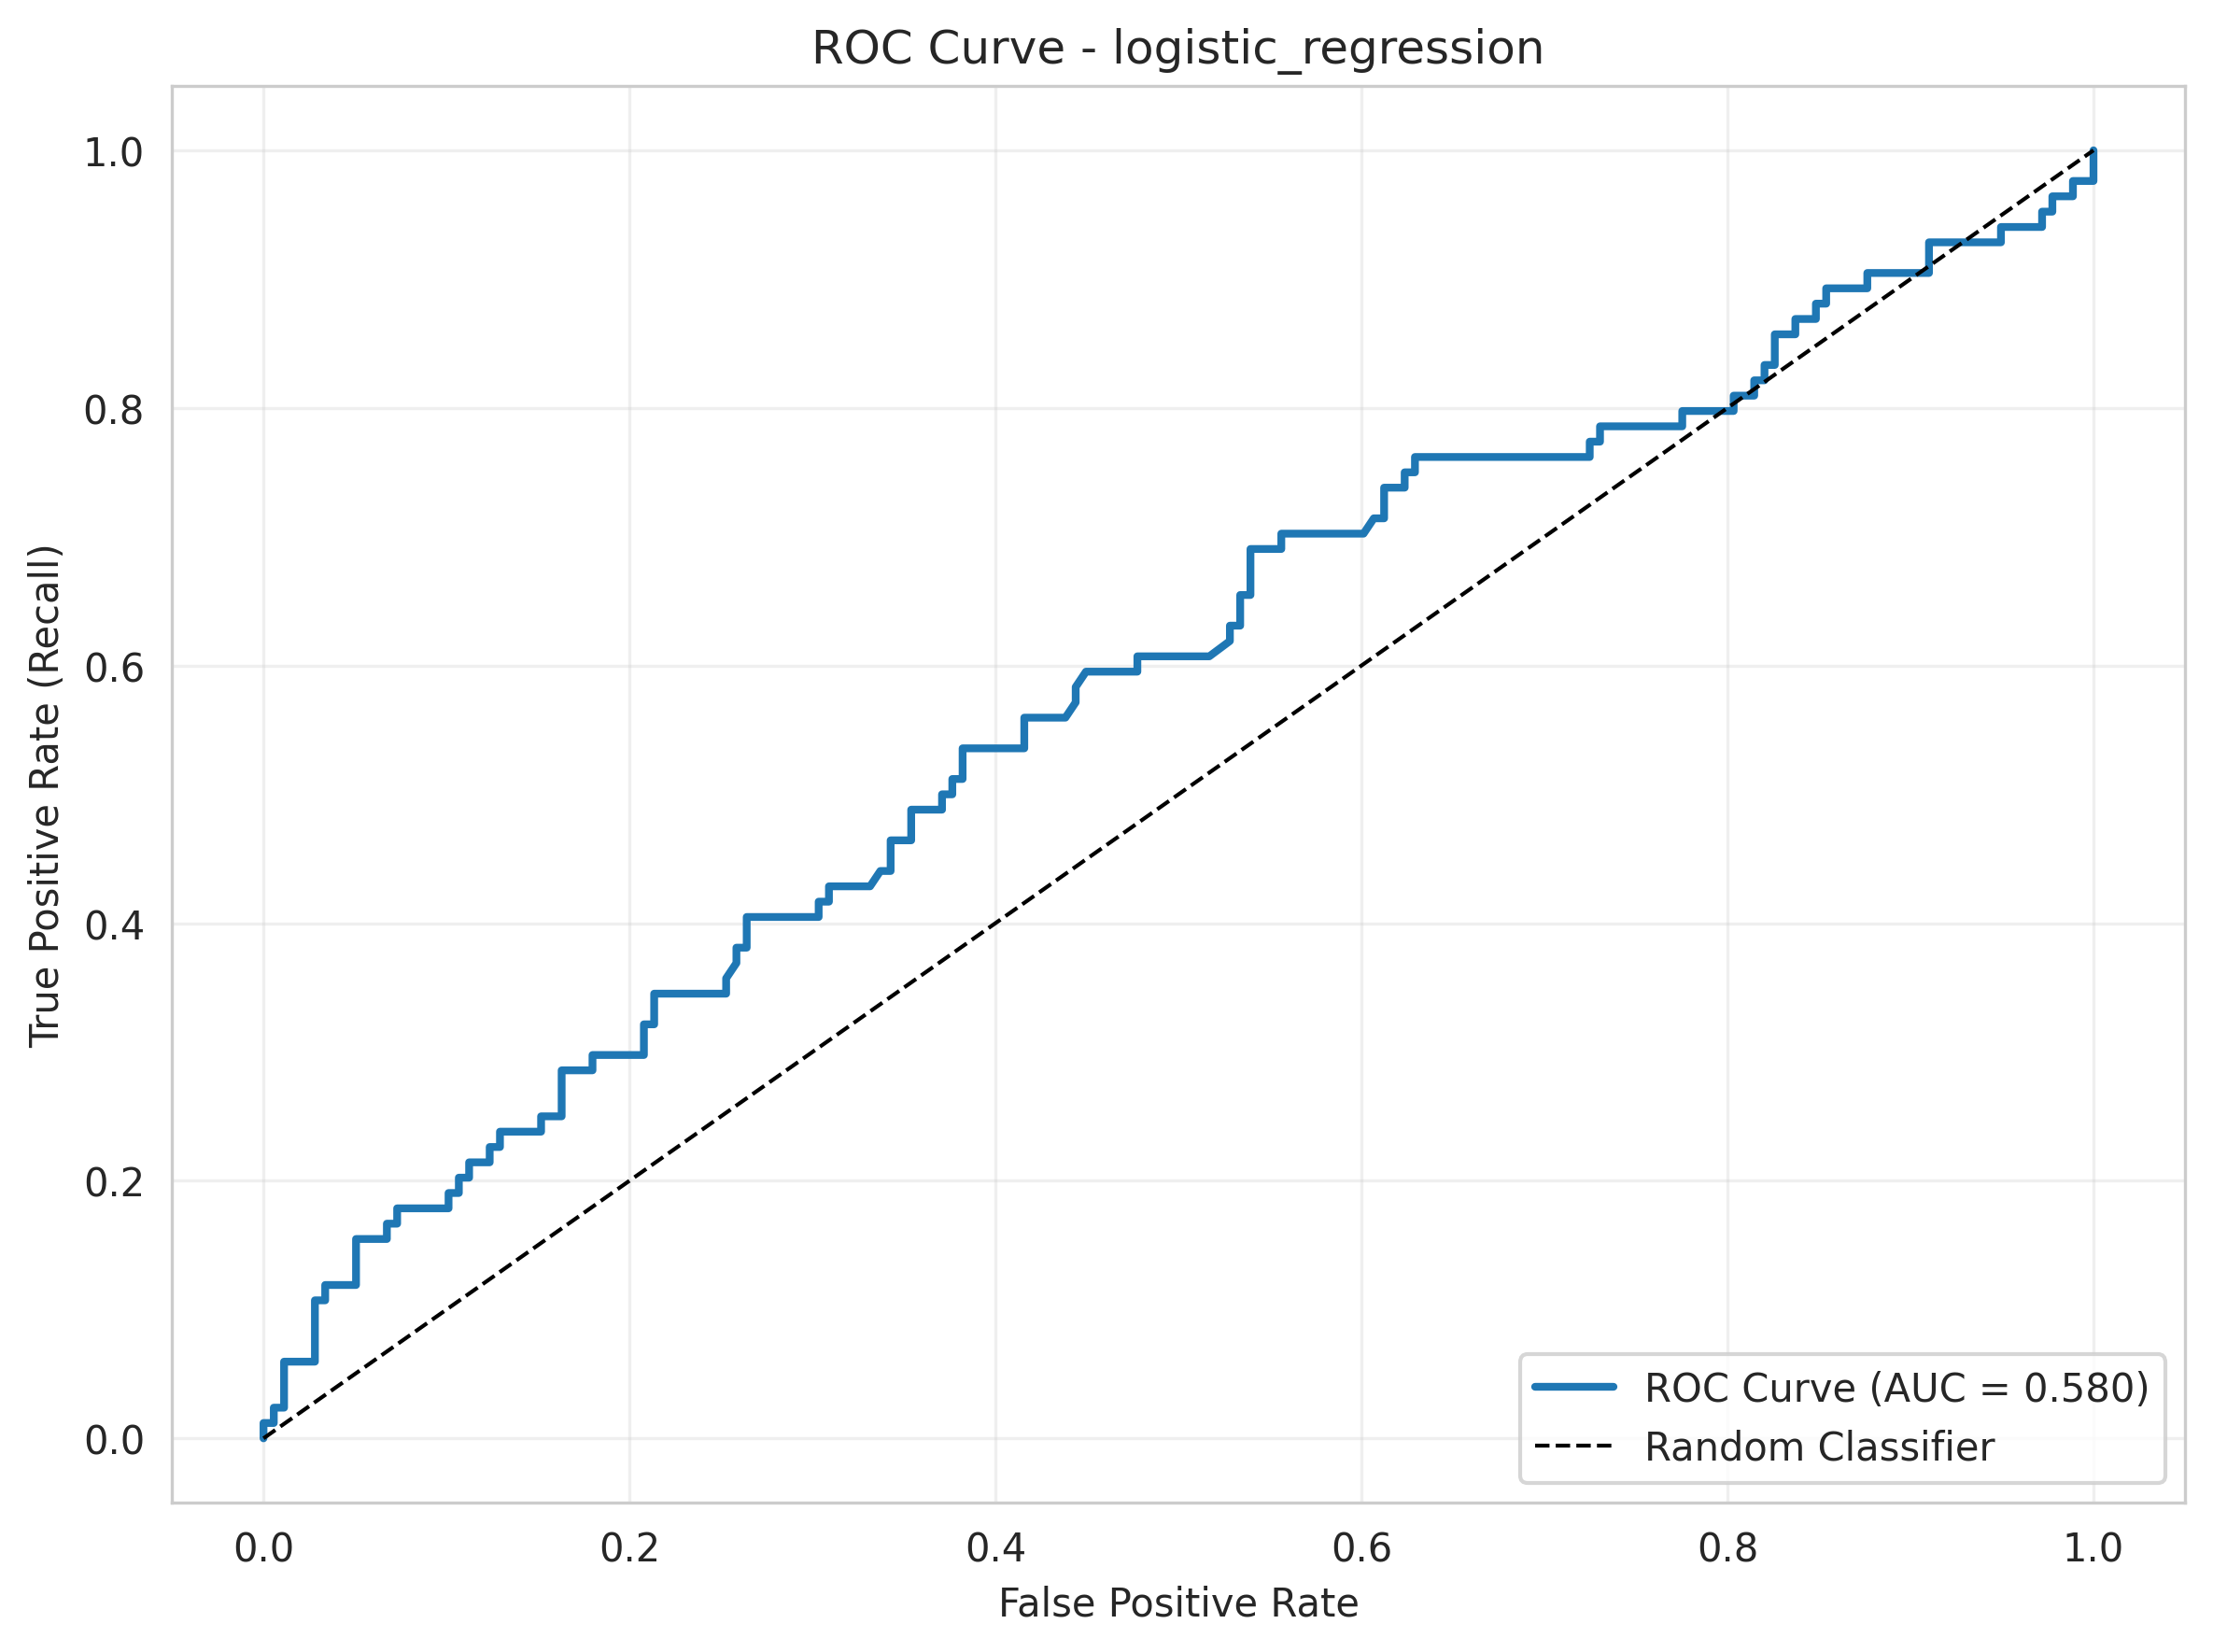
\includegraphics[width=0.8\textwidth]{images/exp_base_roc.png}
\caption{Curva ROC del experimento base (Regresión Logística). El AUC de 0.58 indica capacidad discriminativa marginal.}
\label{fig:exp-base-roc}
\end{figure}

\begin{figure}[H]
\centering
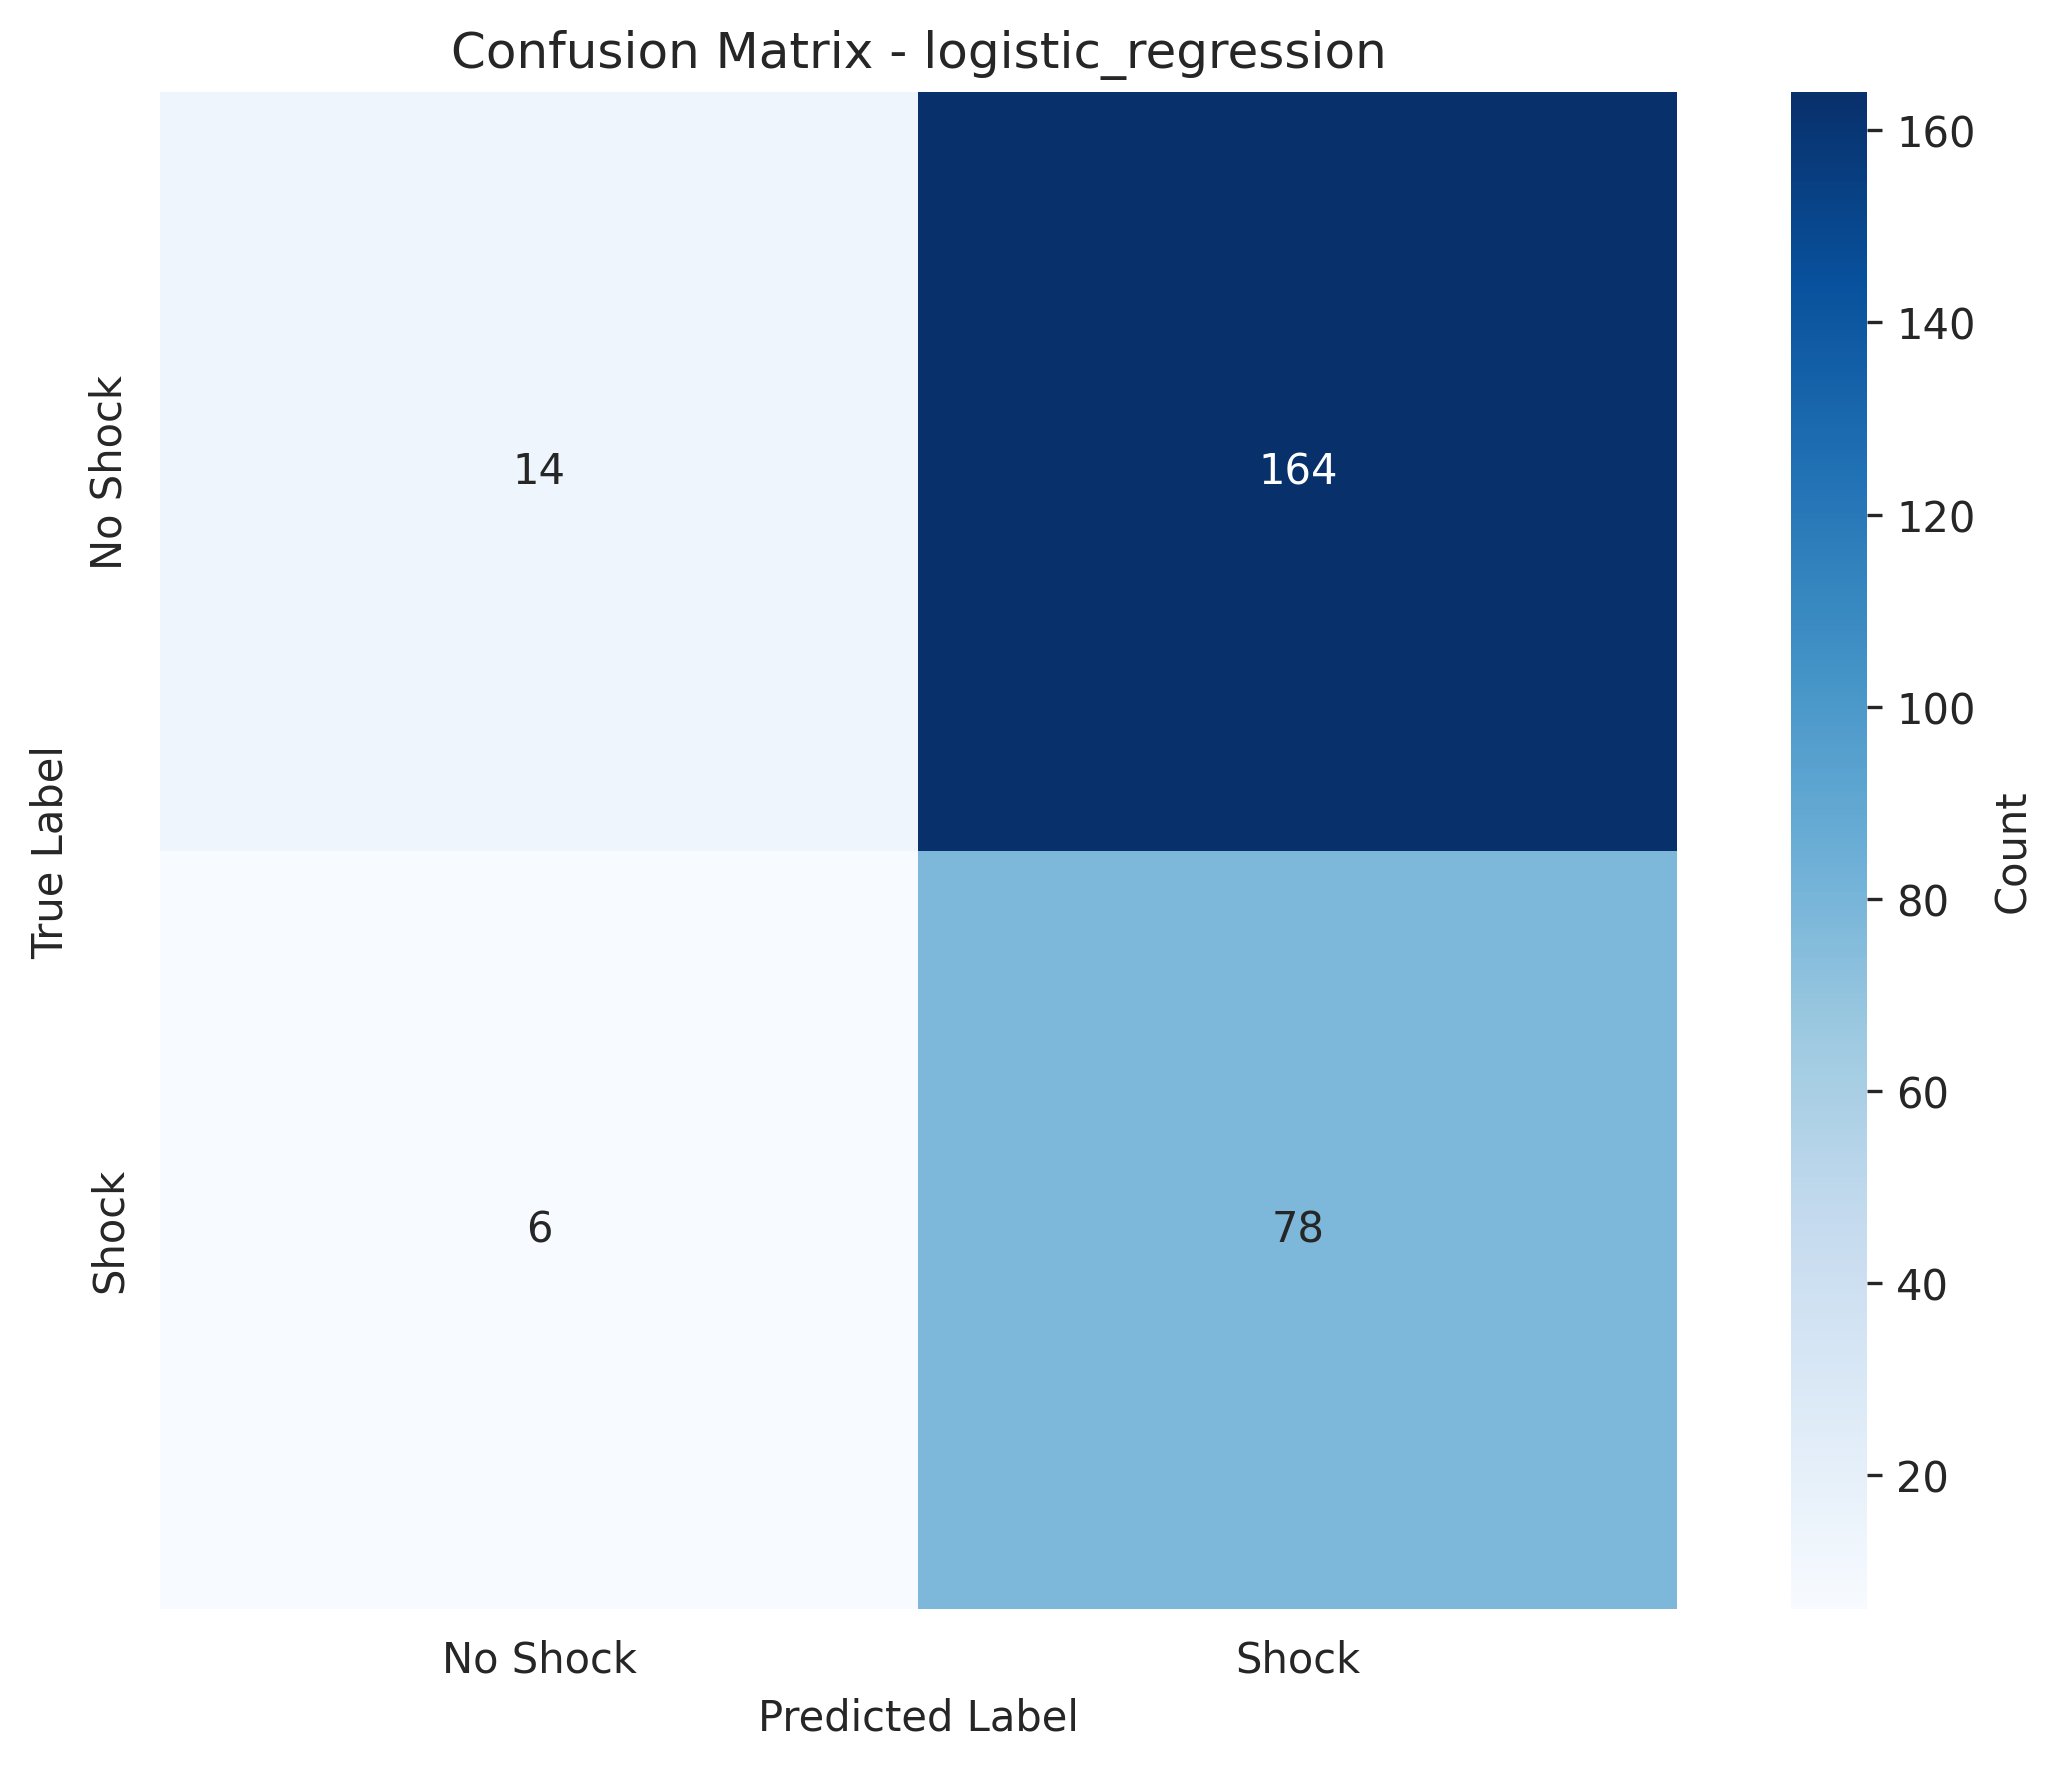
\includegraphics[width=0.65\textwidth]{images/exp_base_confusion.png}
\caption{Matriz de confusión del experimento base. Se observa el sesgo hacia la clase positiva con alta tasa de falsos positivos.}
\label{fig:exp-base-confusion}
\end{figure}

\subsubsection{Efecto de la categorización}

En el segundo experimento se incorporaron las variables categorizadas CATEGORIA\_EDAD y CATEGORIA\_HB\_PREQX, manteniendo las características originales.

\begin{table}[H]
\centering
\caption{Resultados del experimento con categorización}
\label{tab:exp-categ}
\begin{tabular}{|l|c|c|c|c|c|}
\hline
\textbf{Modelo} & \textbf{Recall} & \textbf{Precisión} & \textbf{Especificidad} & \textbf{F1-Score} & \textbf{AUC-ROC} \\ \hline
Regresión Logística & 0.917 & 0.320 & 0.090 & 0.474 & 0.578 \\ \hline
Random Forest & 0.726 & 0.337 & 0.320 & 0.460 & 0.531 \\ \hline
Gradient Boosting & 0.238 & 0.345 & 0.787 & 0.282 & 0.530 \\ \hline
\end{tabular}
\end{table}

La categorización no produjo mejoras significativas en el rendimiento. Los resultados fueron prácticamente idénticos al experimento base, indicando que la transformación de variables continuas a categóricas no aporta información adicional discriminativa por sí sola.

\begin{figure}[H]
\centering
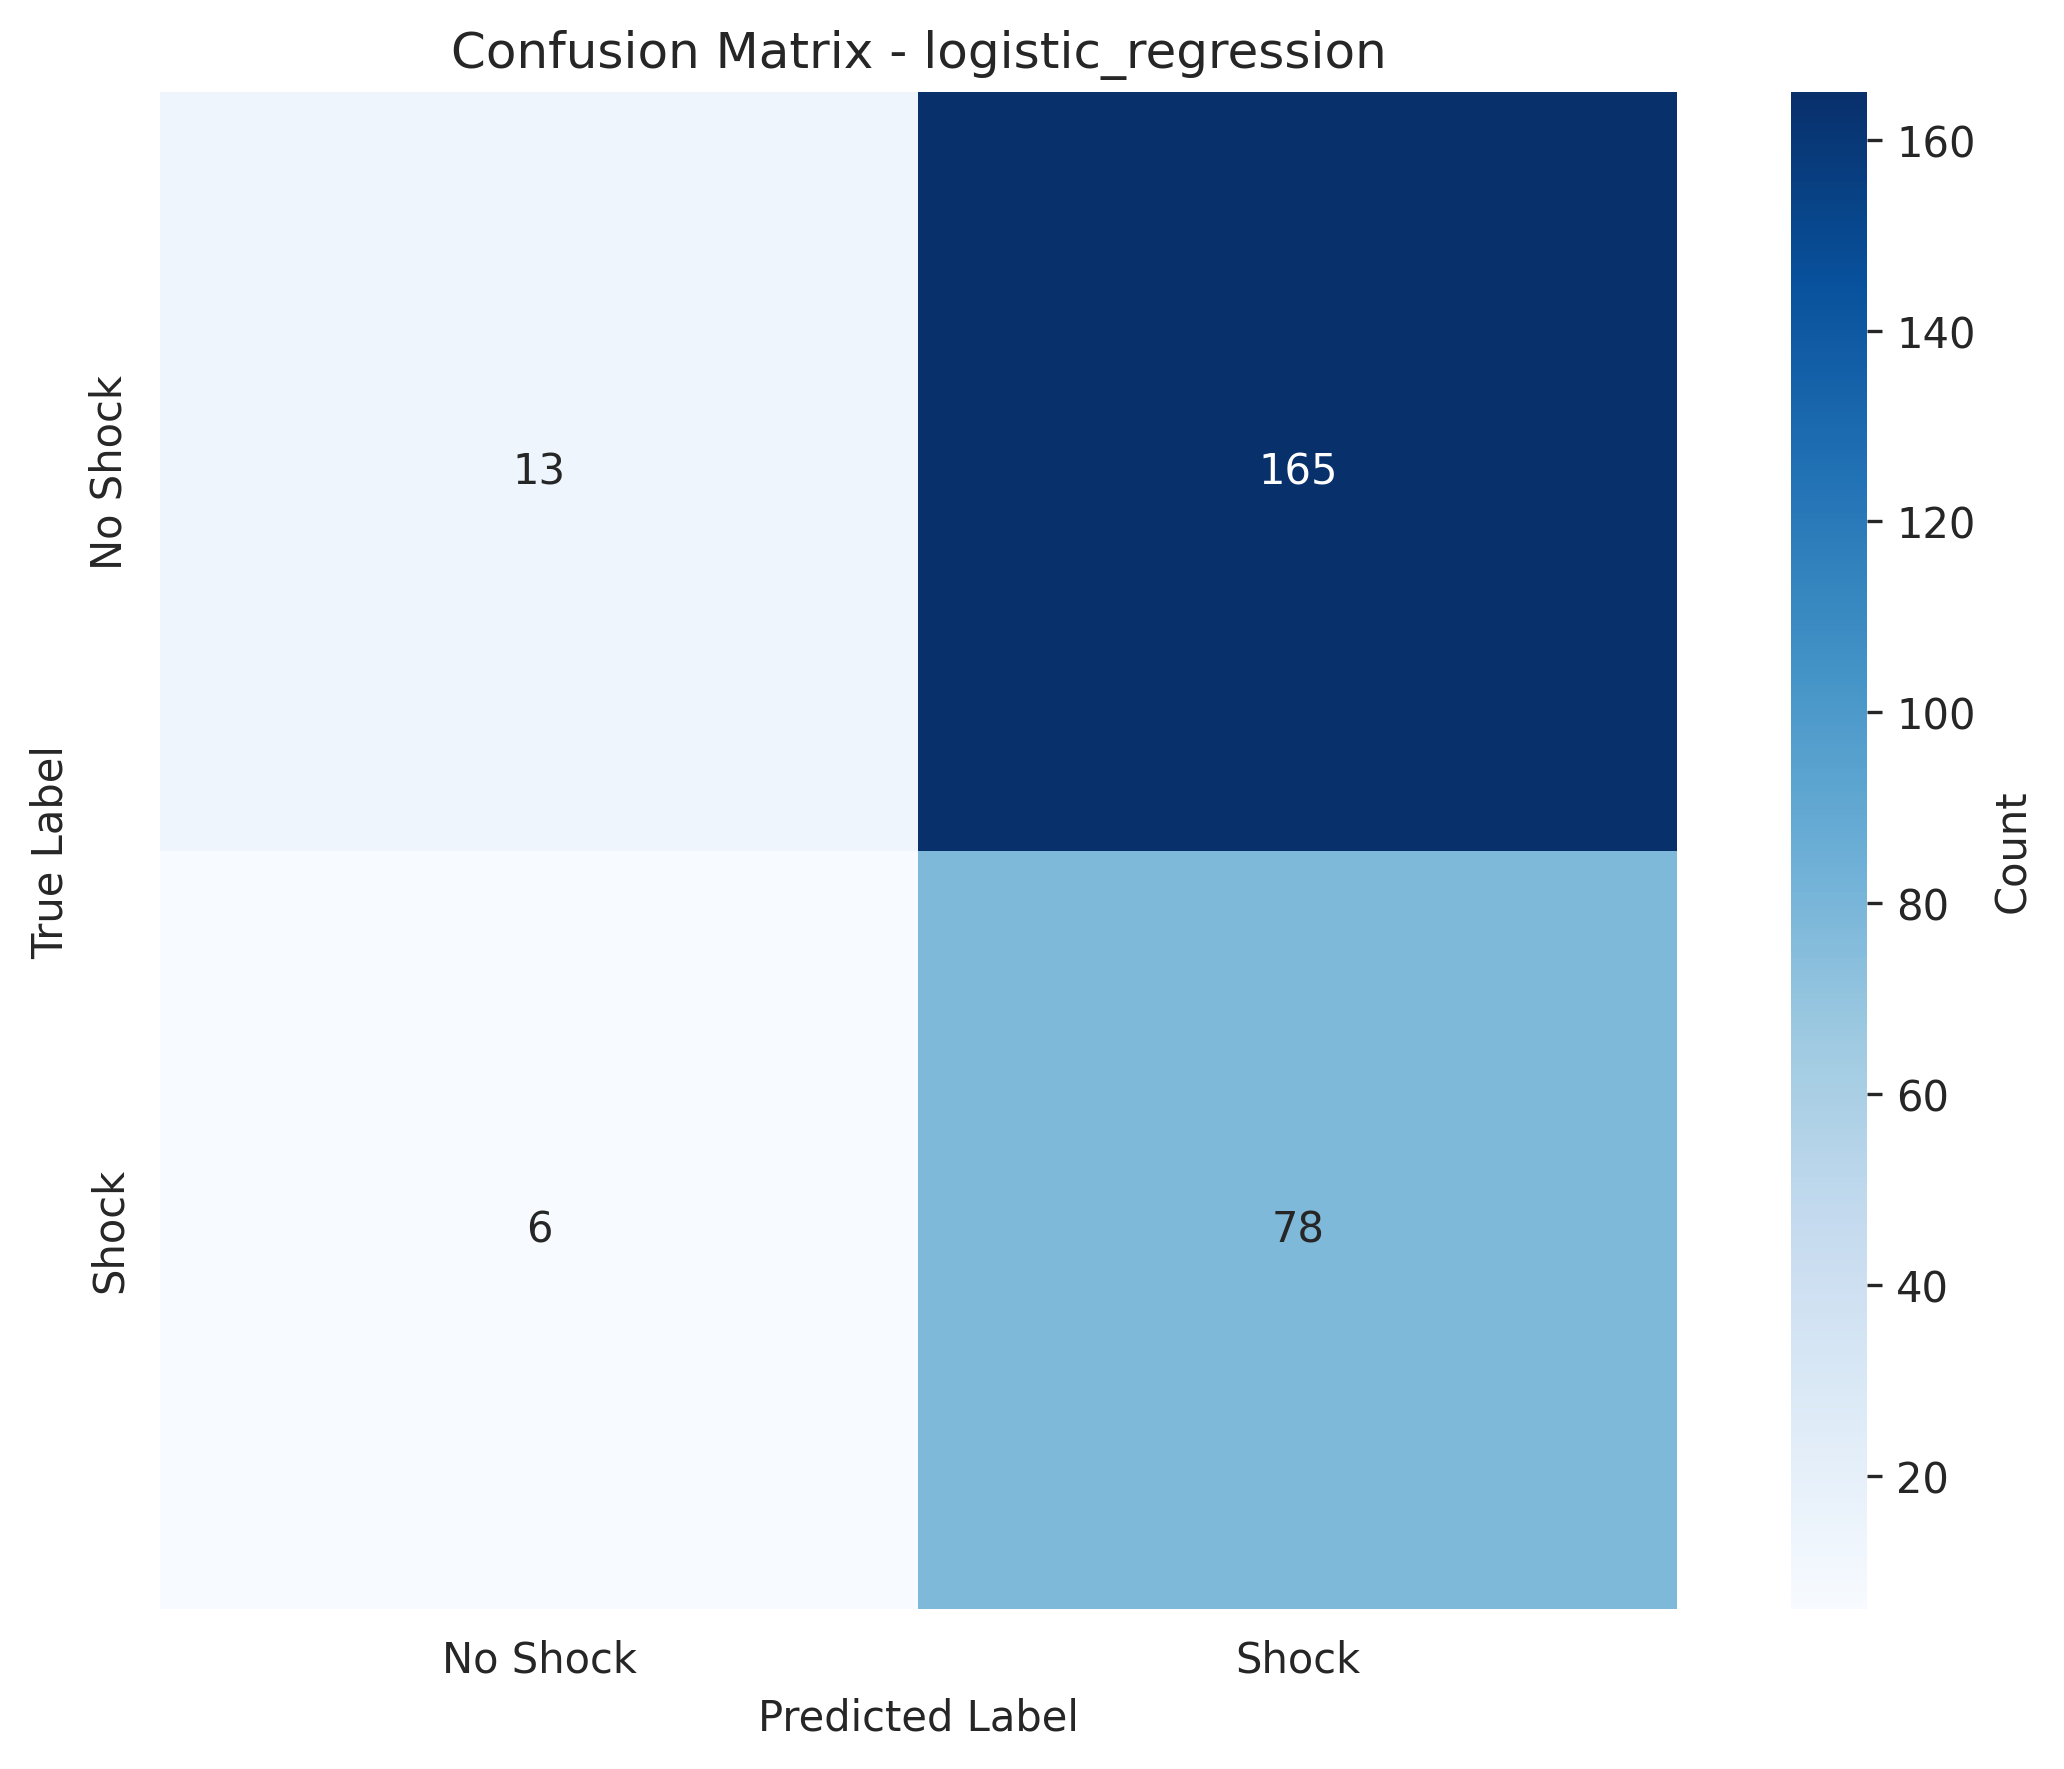
\includegraphics[width=0.65\textwidth]{images/exp_categ_confusion.png}
\caption{Matriz de confusión del experimento con categorización (Regresión Logística). Patrón similar al experimento base.}
\label{fig:categ-confusion}
\end{figure}

\subsubsection{Efecto de las agregaciones clínicas}

En el tercer experimento se añadieron al dataset las variables agregadas: CARGA\_COMORBILIDADES, FACTORES\_RIESGO\_SANGRADO y SANGRADO\_X\_CV. Estas variables se sumaron a las características originales para evaluar si la combinación de comorbilidades en índices compuestos podía mejorar la capacidad predictiva.

\begin{table}[H]
\centering
\caption{Resultados del experimento con agregaciones}
\label{tab:exp-agreg}
\begin{tabular}{|l|c|c|c|c|c|}
\hline
\textbf{Modelo} & \textbf{Recall} & \textbf{Precisión} & \textbf{Especificidad} & \textbf{F1-Score} & \textbf{AUC-ROC} \\ \hline
Regresión Logística & 0.905 & 0.319 & 0.107 & 0.472 & 0.573 \\ \hline
Random Forest & 0.702 & 0.339 & 0.343 & 0.457 & 0.530 \\ \hline
Gradient Boosting & 0.190 & 0.296 & 0.787 & 0.232 & 0.528 \\ \hline
\end{tabular}
\end{table}

Las agregaciones clínicas tampoco produjeron mejoras sustanciales. Sin embargo, se observó que la variable CARGA\_COMORBILIDADES mostró un valor P significativo (4.54e-09) y un Cohen's d de 0.282, lo que sugiere relevancia estadística aunque no se tradujo en mejora del rendimiento predictivo en este experimento.

\begin{figure}[H]
\centering
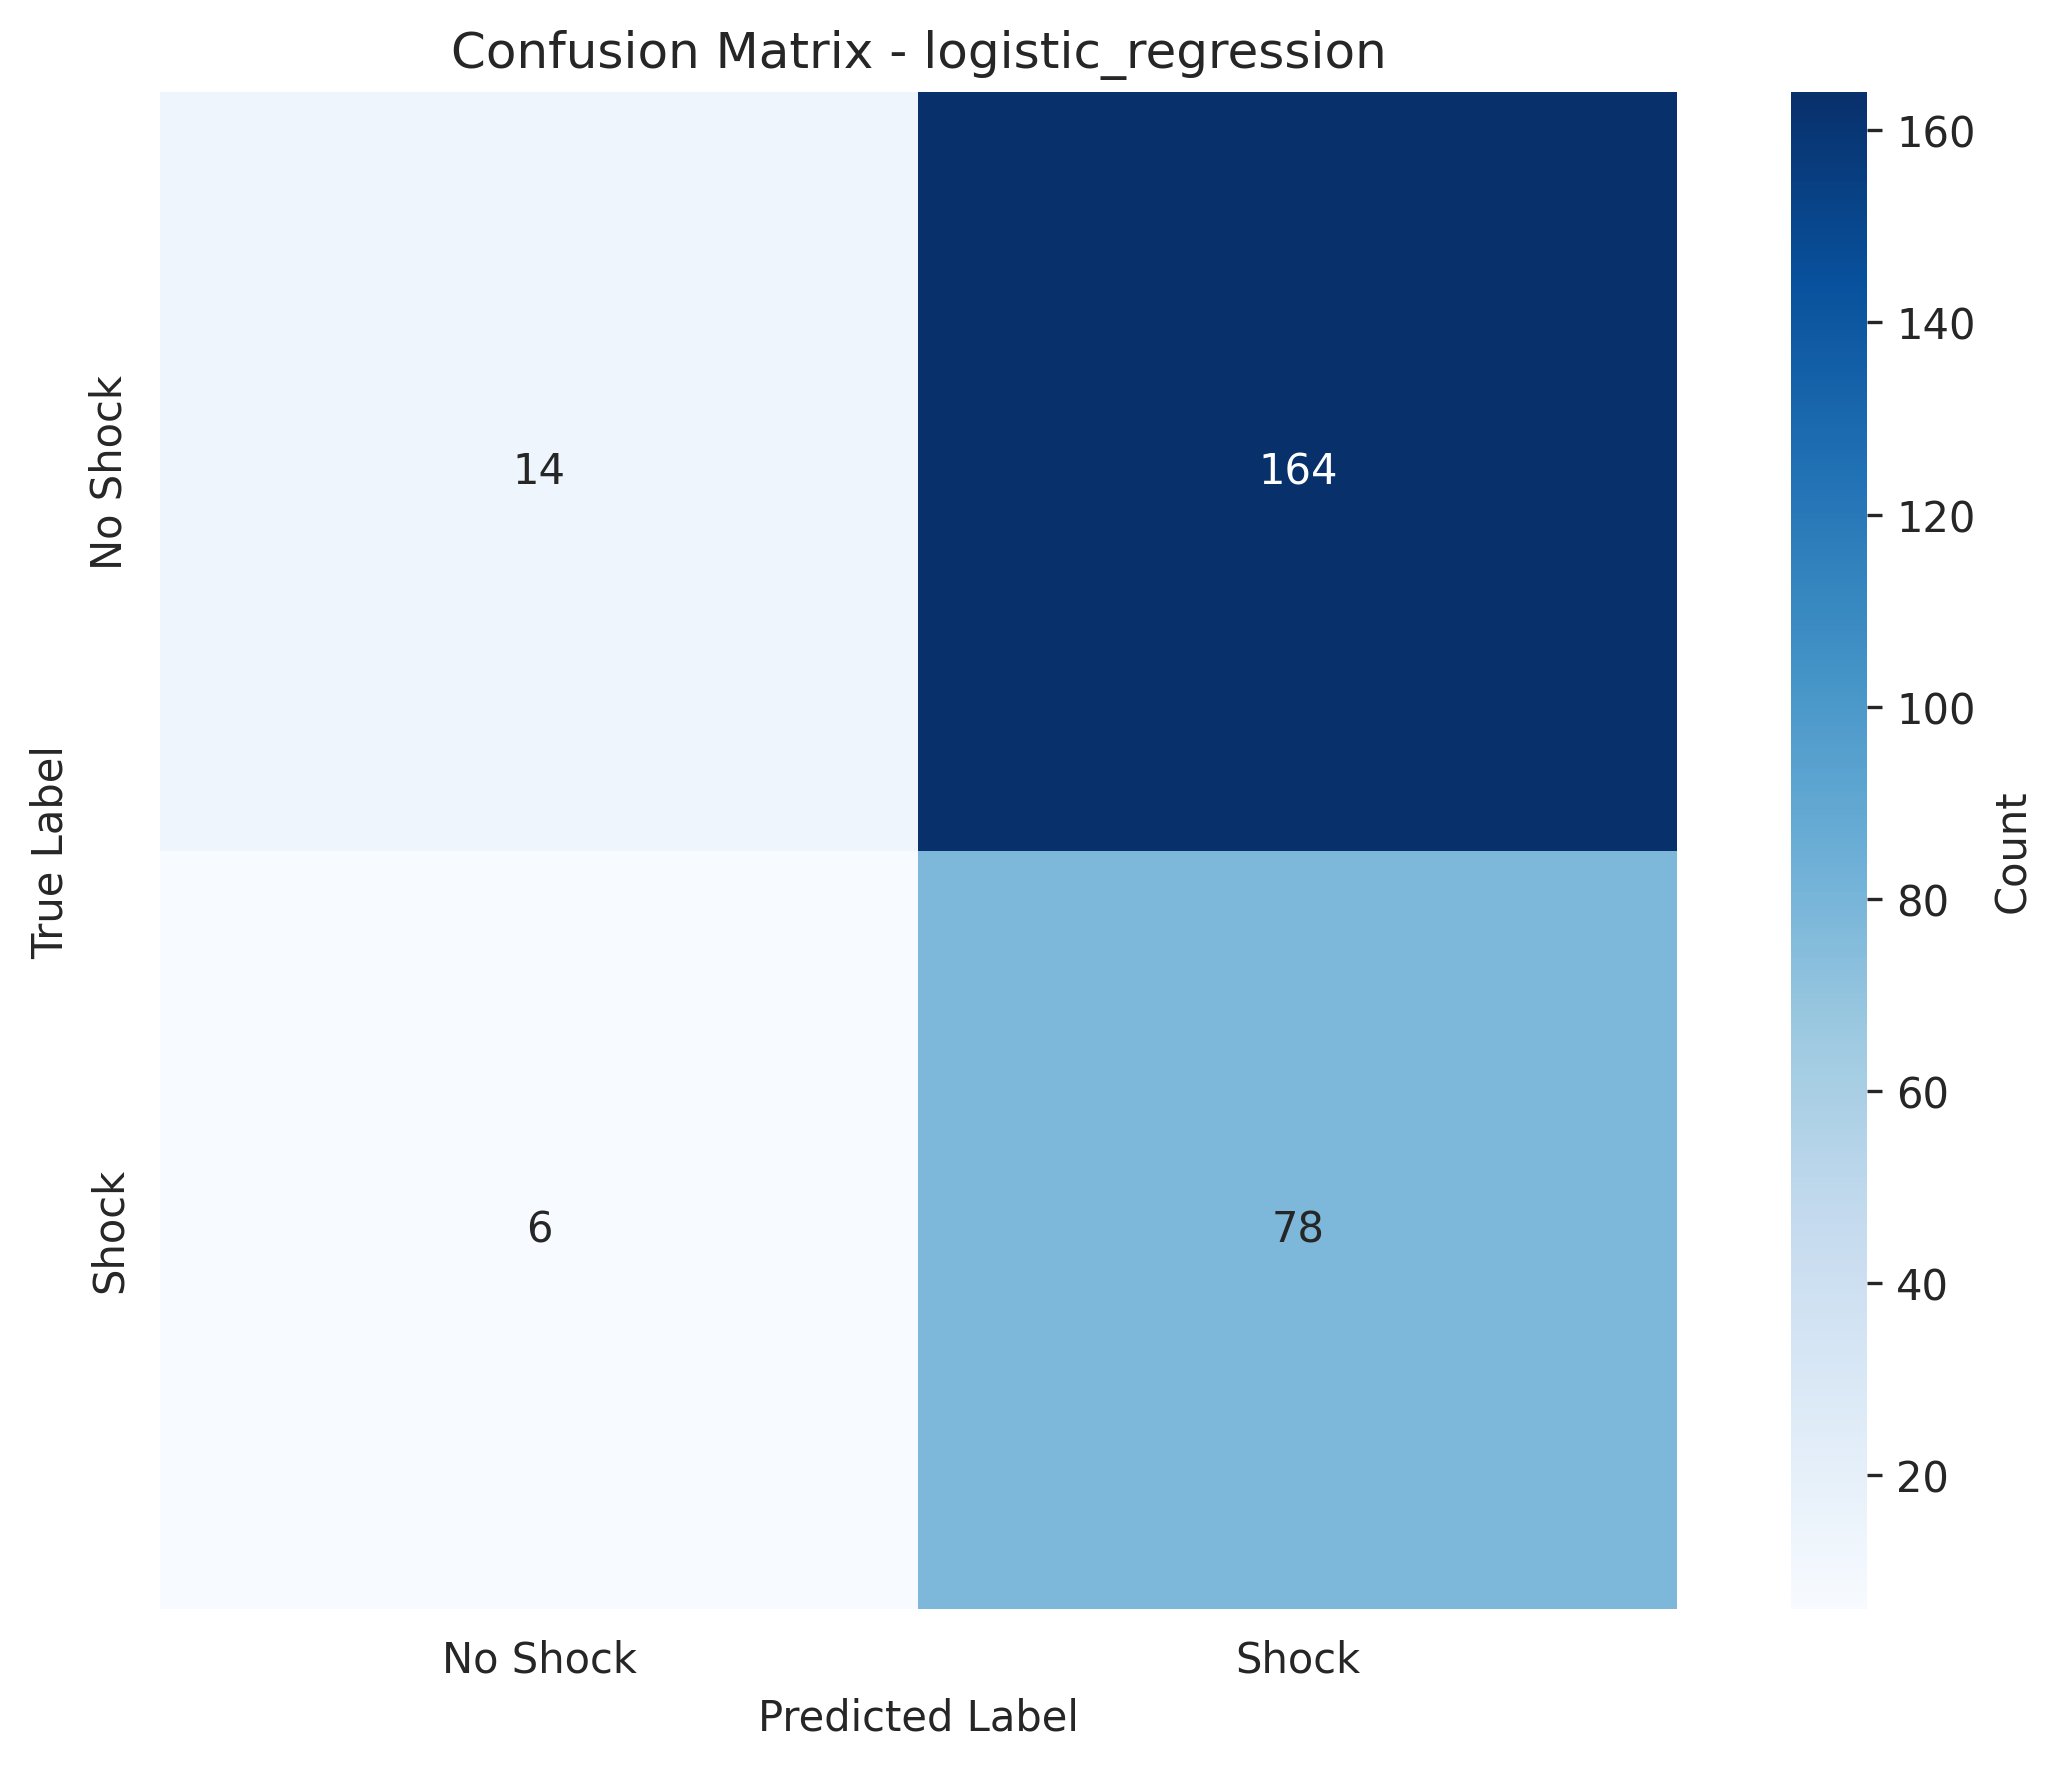
\includegraphics[width=0.65\textwidth]{images/exp_agreg_confusion.png}
\caption{Matriz de confusión del experimento con agregaciones (Regresión Logística). El patrón de clasificación permanece sin cambios significativos.}
\label{fig:agreg-confusion}
\end{figure}

\subsubsection{Combinación de categorización y agregaciones}

El cuarto experimento combinó ambas estrategias de ingeniería de características.

\begin{table}[H]
\centering
\caption{Resultados del experimento combinado}
\label{tab:exp-combinado}
\begin{tabular}{|l|c|c|c|c|c|}
\hline
\textbf{Modelo} & \textbf{Recall} & \textbf{Precisión} & \textbf{Especificidad} & \textbf{F1-Score} & \textbf{AUC-ROC} \\ \hline
Regresión Logística & 0.893 & 0.317 & 0.118 & 0.468 & 0.571 \\ \hline
Random Forest & 0.690 & 0.340 & 0.354 & 0.456 & 0.529 \\ \hline
Gradient Boosting & 0.214 & 0.321 & 0.787 & 0.257 & 0.526 \\ \hline
\end{tabular}
\end{table}

La combinación de ambas estrategias no superó el rendimiento de los experimentos individuales. Esto sugiere que las características derivadas introducen redundancia sin aportar información discriminativa adicional para la tarea de predicción.

\begin{figure}[H]
\centering
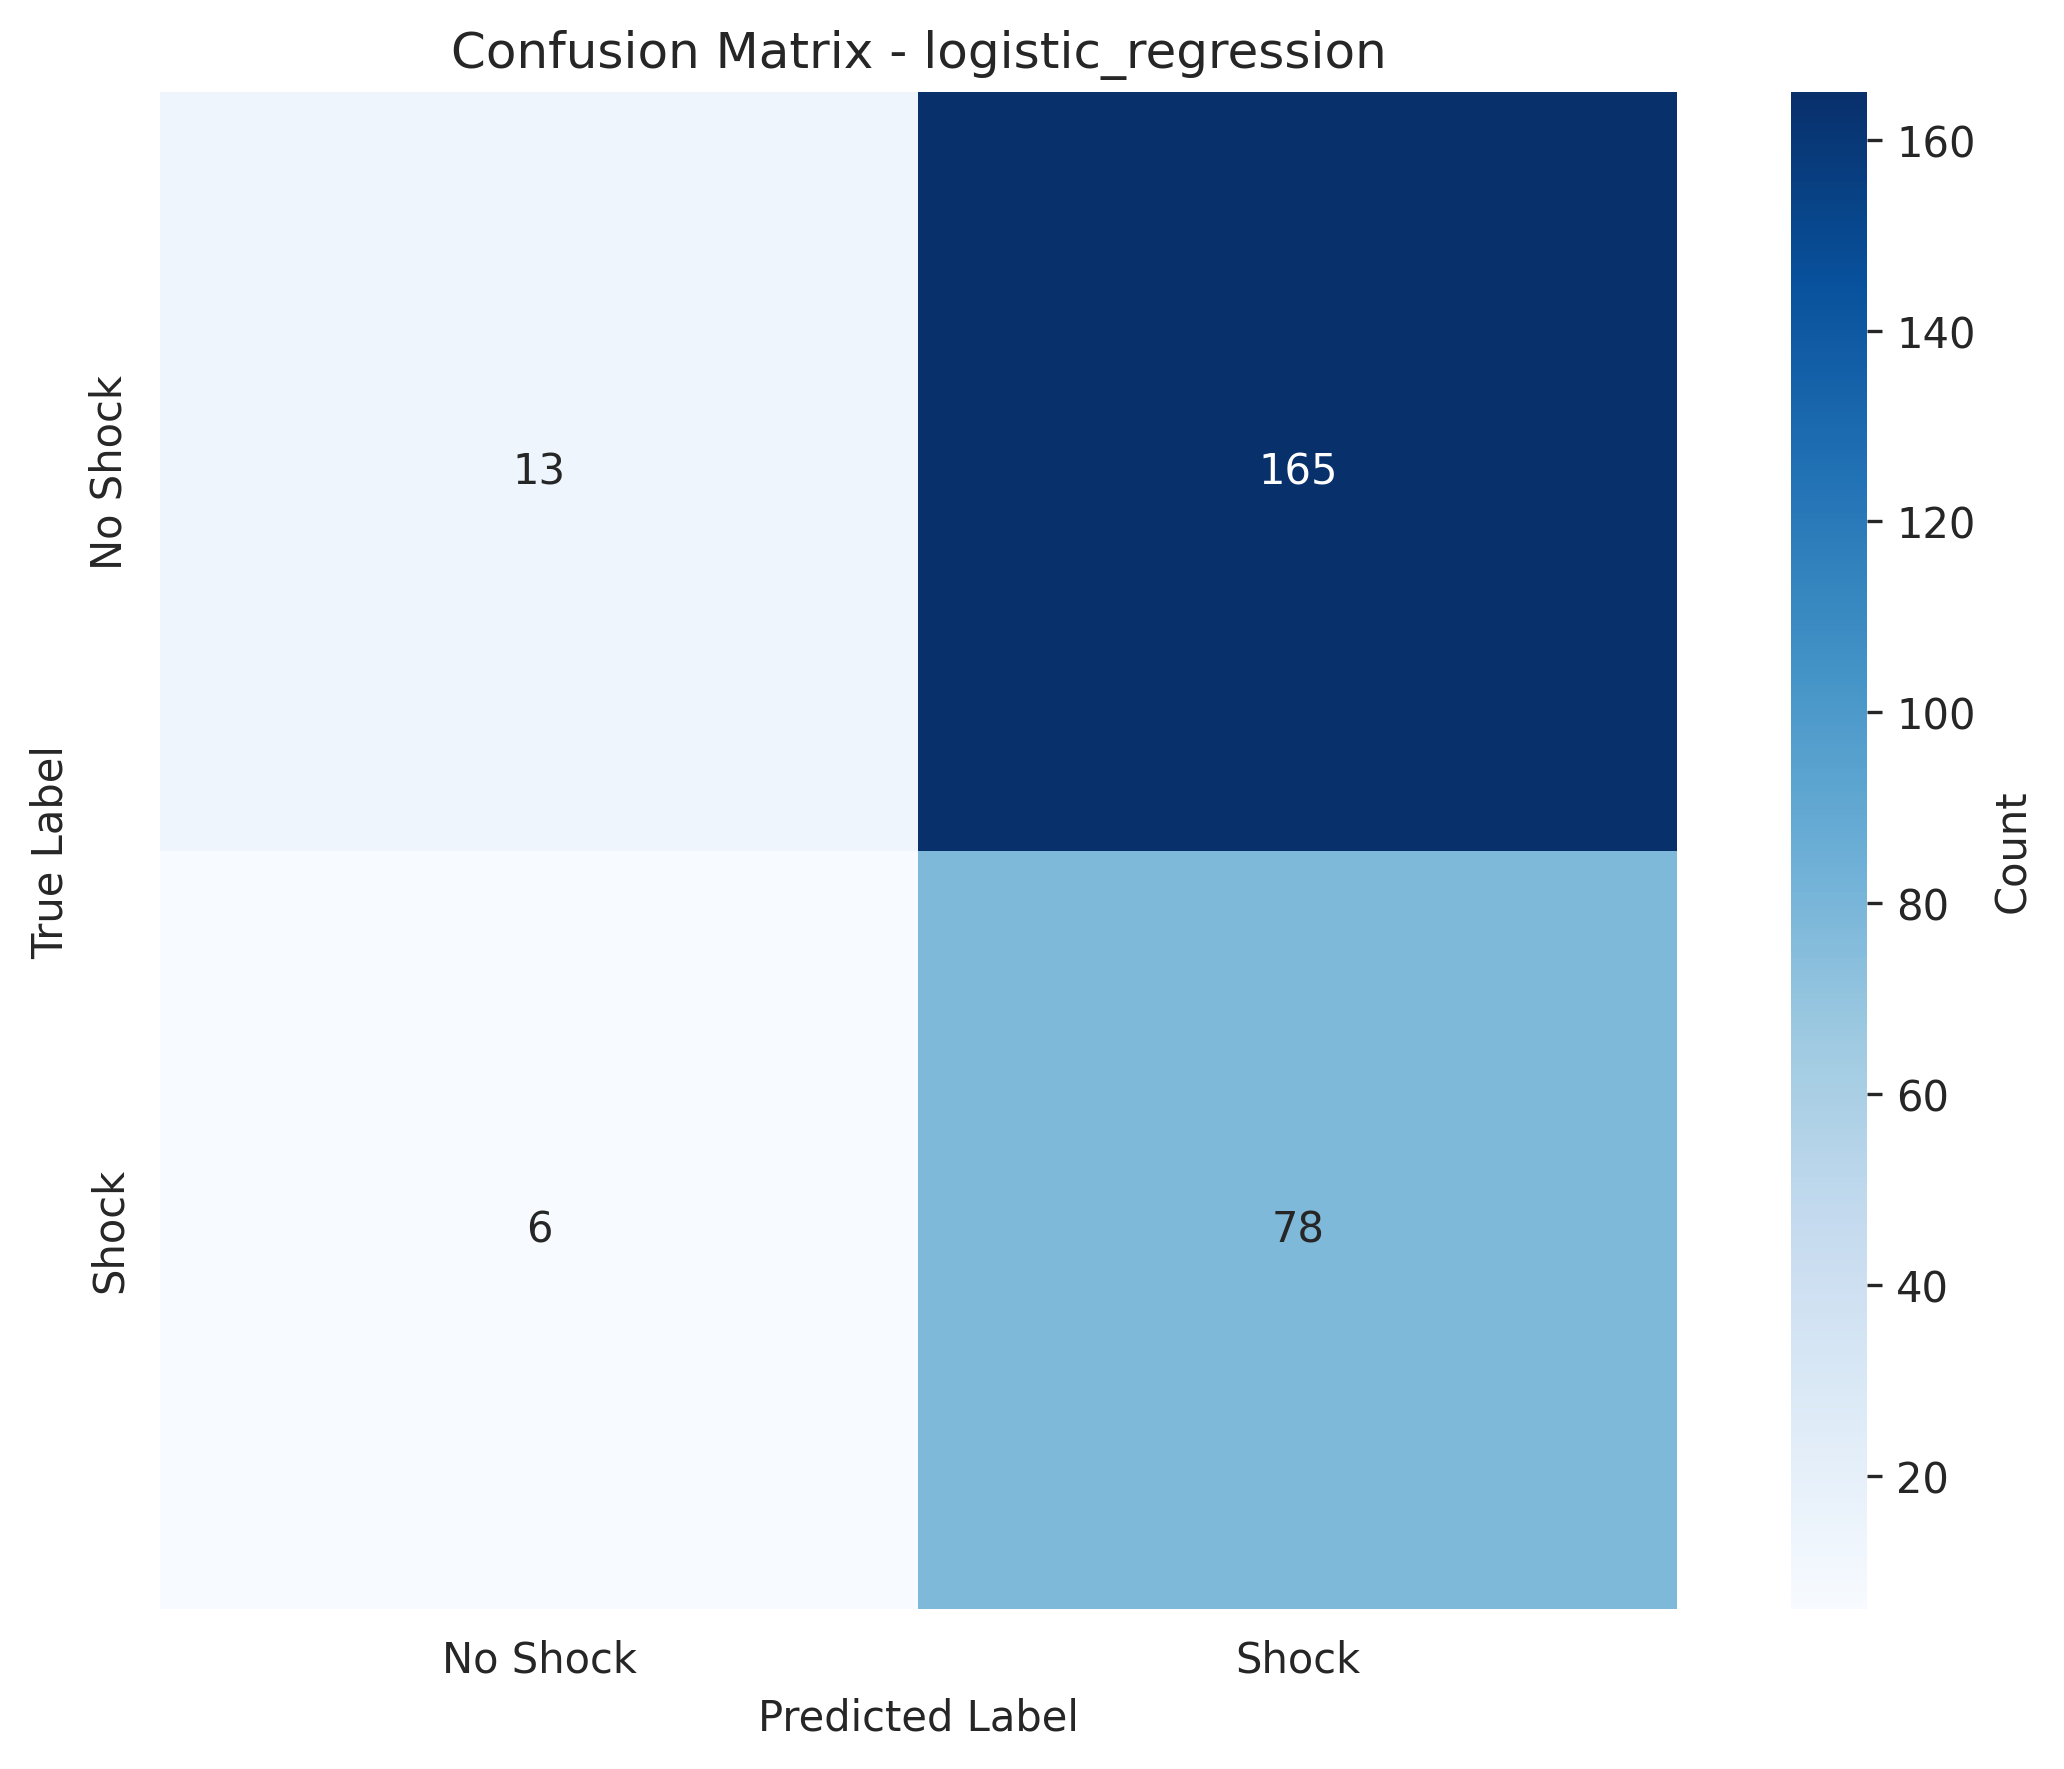
\includegraphics[width=0.65\textwidth]{images/exp_combi_confusion.png}
\caption{Matriz de confusión del experimento combinado (Regresión Logística). La combinación de técnicas no mejora la discriminación.}
\label{fig:combi-confusion}
\end{figure}

\subsubsection{Ajuste de hiperparámetros}

En los siguientes experimentos, se realizó una búsqueda sistemática de hiperparámetros óptimos para cada modelo. Se utilizó búsqueda en grilla con validación cruzada para optimizar parámetros como:

\begin{itemize}
    \item \textbf{Gradient Boosting:} learning\_rate, n\_estimators, max\_depth, min\_samples\_split.
    \item \textbf{Random Forest:} n\_estimators, max\_depth, min\_samples\_leaf, class\_weight.
    \item \textbf{Regresión Logística:} C (regularización), penalty, solver.
\end{itemize}

\begin{table}[H]
\centering
\caption{Mejores resultados con ajuste de hiperparámetros}
\label{tab:exp-hyperparams}
\begin{tabular}{|l|c|c|c|c|}
\hline
\textbf{Modelo} & \textbf{Recall} & \textbf{Precisión} & \textbf{AUC-ROC} & \textbf{F1-Score} \\ \hline
Gradient Boosting (Config. 1) & 0.238 & 0.294 & 0.521 & 0.263 \\ \hline
Gradient Boosting (Config. 2) & 0.155 & 0.382 & 0.560 & 0.220 \\ \hline
Gradient Boosting (Config. 3) & 0.214 & 0.333 & 0.540 & 0.260 \\ \hline
\end{tabular}
\end{table}

El ajuste de hiperparámetros produjo mejoras marginales en AUC-ROC, pero no logró superar significativamente el rendimiento base. Esto confirmó que el problema principal residía en la capacidad discriminativa inherente de las características, no en la configuración de los modelos.

\begin{figure}[H]
\centering
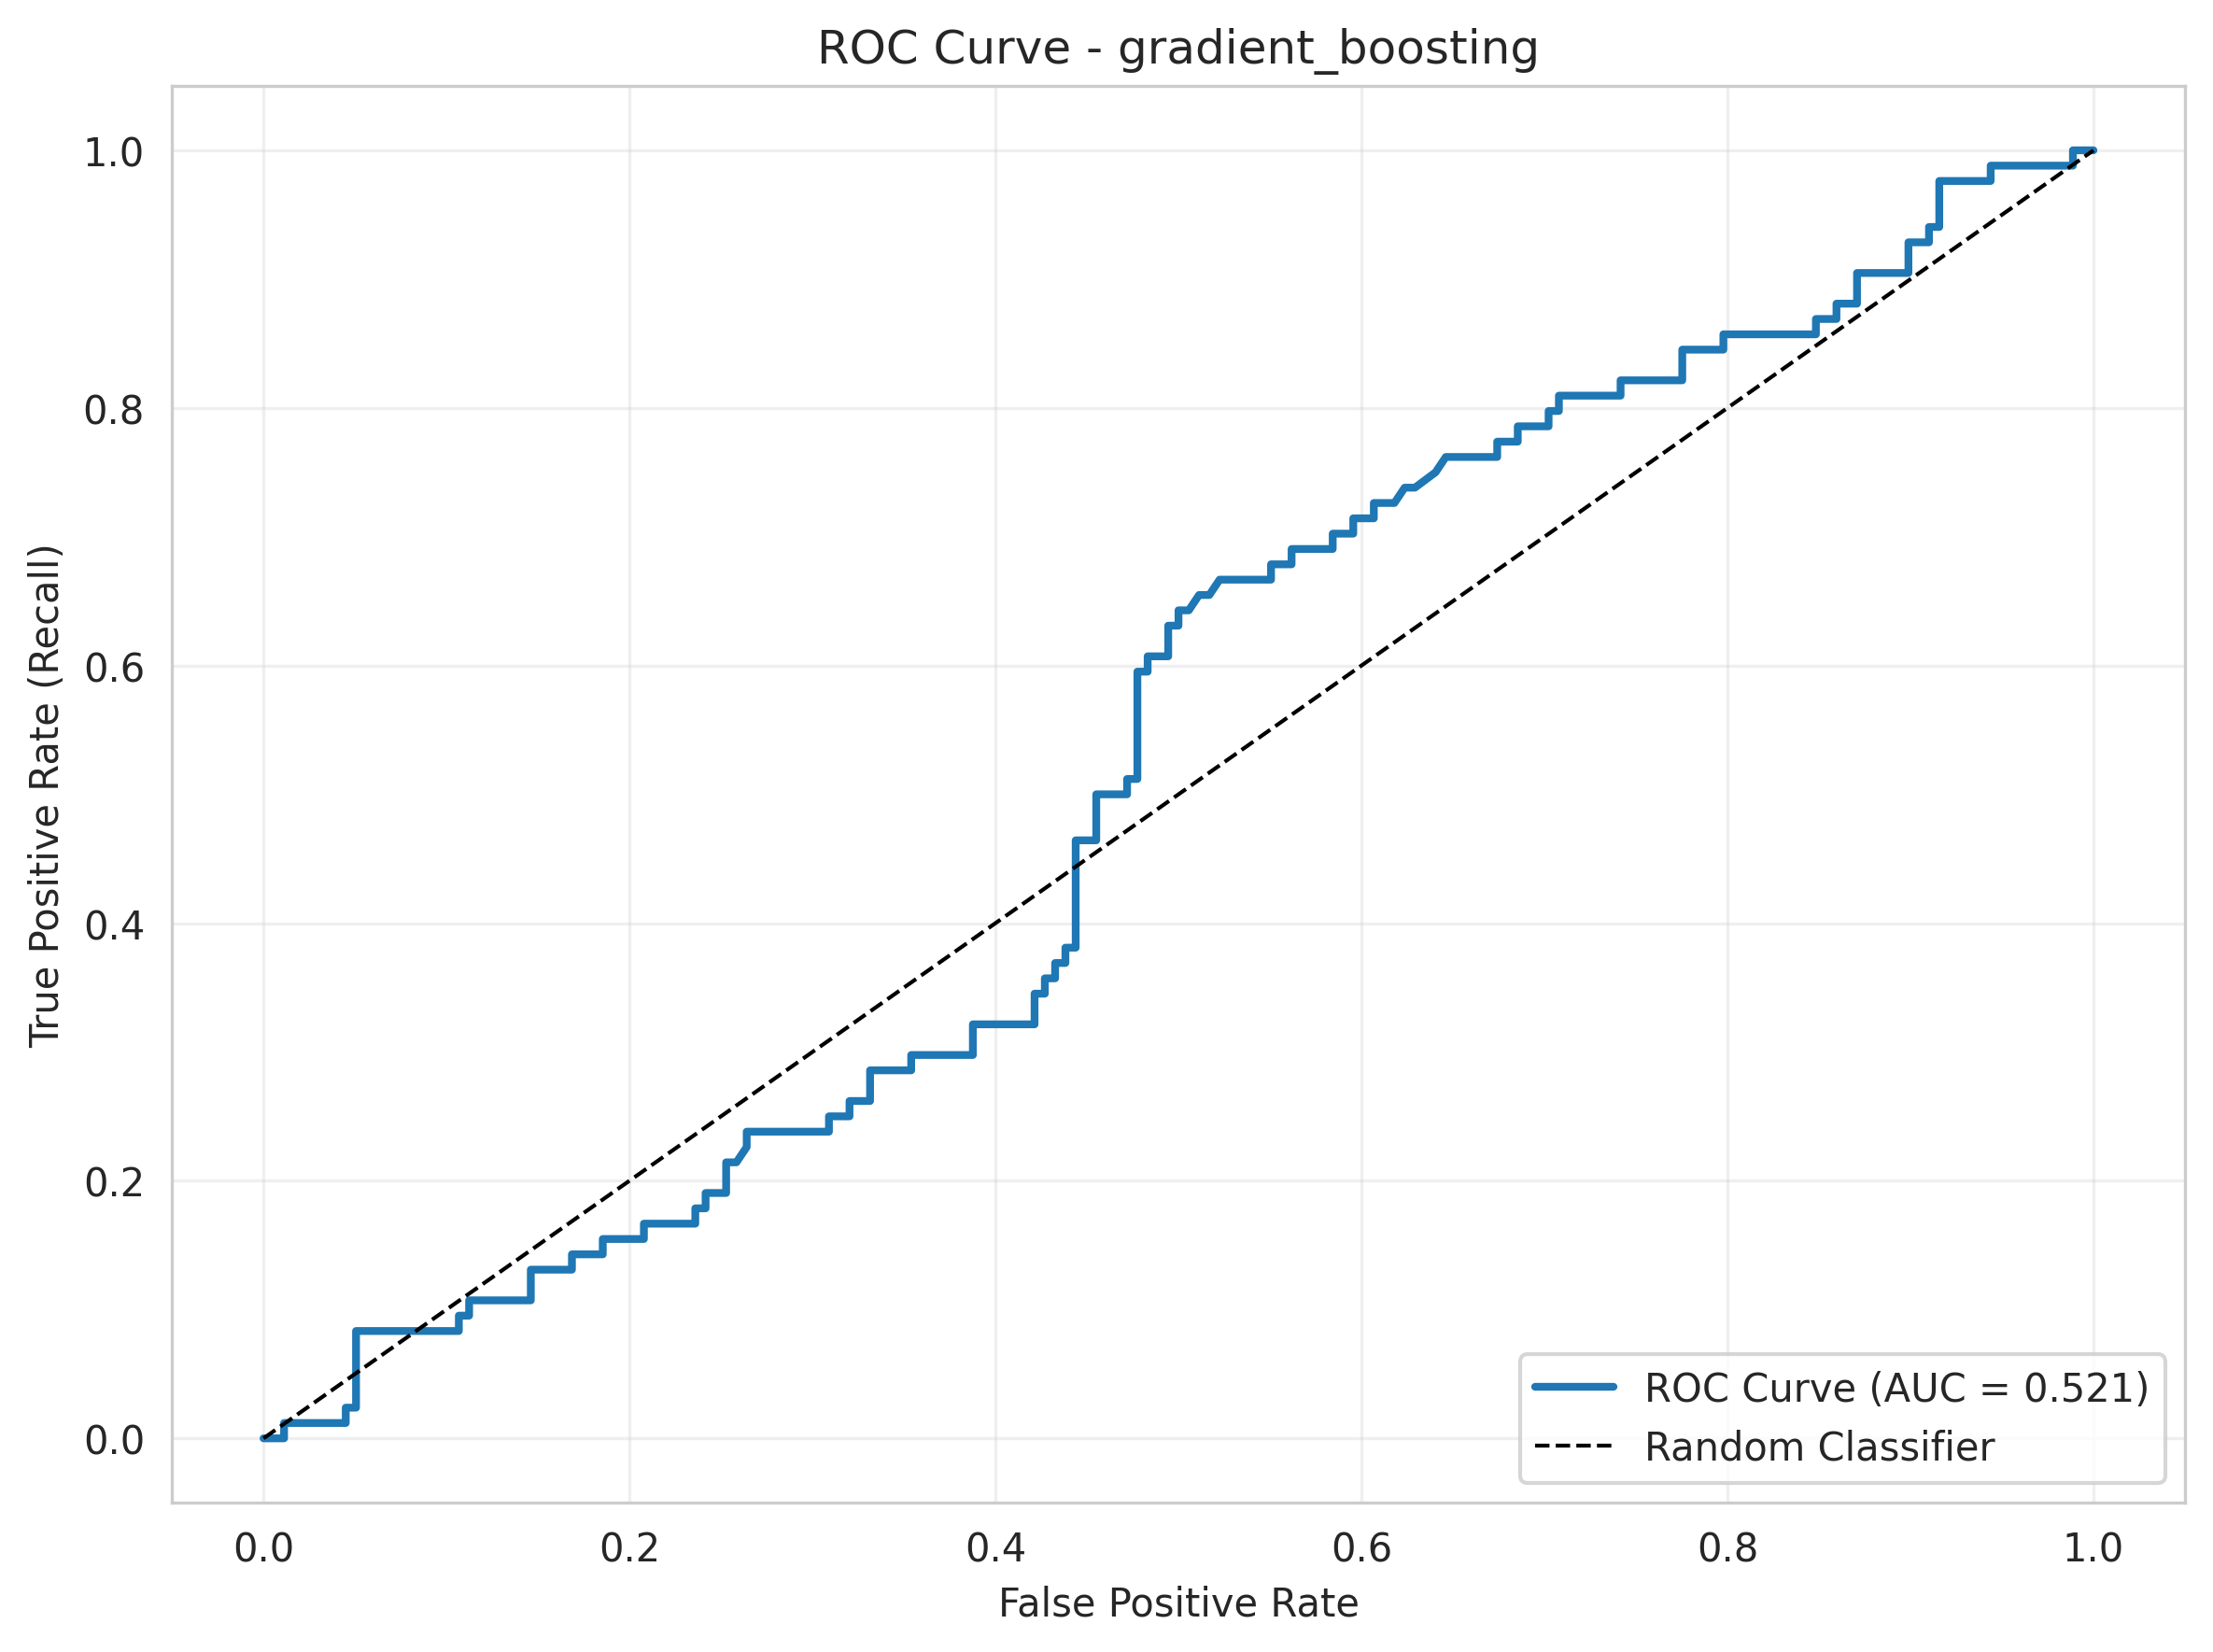
\includegraphics[width=0.8\textwidth]{images/exp_hyper_roc.png}
\caption{Curva ROC de Gradient Boosting tras ajuste de hiperparámetros. AUC de 0.521, mejora marginal.}
\label{fig:hyper-roc}
\end{figure}

\subsubsection{Incorporación de nuevos modelos}

En experimentos posteriores, se amplió el repertorio de algoritmos incorporando K-Nearest Neighbors (KNN) y LightGBM. Esta decisión se fundamentó en:

\begin{itemize}
    \item \textbf{KNN:} Modelo no paramétrico que puede capturar relaciones locales en los datos.
    \item \textbf{LightGBM:} Implementación eficiente de gradient boosting con mejor manejo de características categóricas y regularización avanzada.
\end{itemize}

\begin{table}[H]
\centering
\caption{Resultados con nuevos modelos}
\label{tab:exp-nuevos-modelos}
\begin{tabular}{|l|c|c|c|c|c|}
\hline
\textbf{Modelo} & \textbf{Recall} & \textbf{Precisión} & \textbf{Especificidad} & \textbf{F1-Score} & \textbf{AUC-ROC} \\ \hline
LightGBM & 0.262 & 0.265 & 0.657 & 0.263 & 0.508 \\ \hline
KNN & 0.238 & 0.282 & 0.713 & 0.258 & 0.492 \\ \hline
Gradient Boosting & 0.238 & 0.323 & 0.764 & 0.274 & 0.543 \\ \hline
Random Forest & 0.262 & 0.282 & 0.685 & 0.271 & 0.516 \\ \hline
Regresión Logística & 0.988 & 0.321 & 0.004 & 0.485 & 0.560 \\ \hline
\end{tabular}
\end{table}

LightGBM y KNN no superaron a los modelos tradicionales. La Regresión Logística continuó mostrando el patrón de clasificar casi todos los casos como positivos (recall muy alto, especificidad cercana a cero).

\begin{figure}[H]
\centering
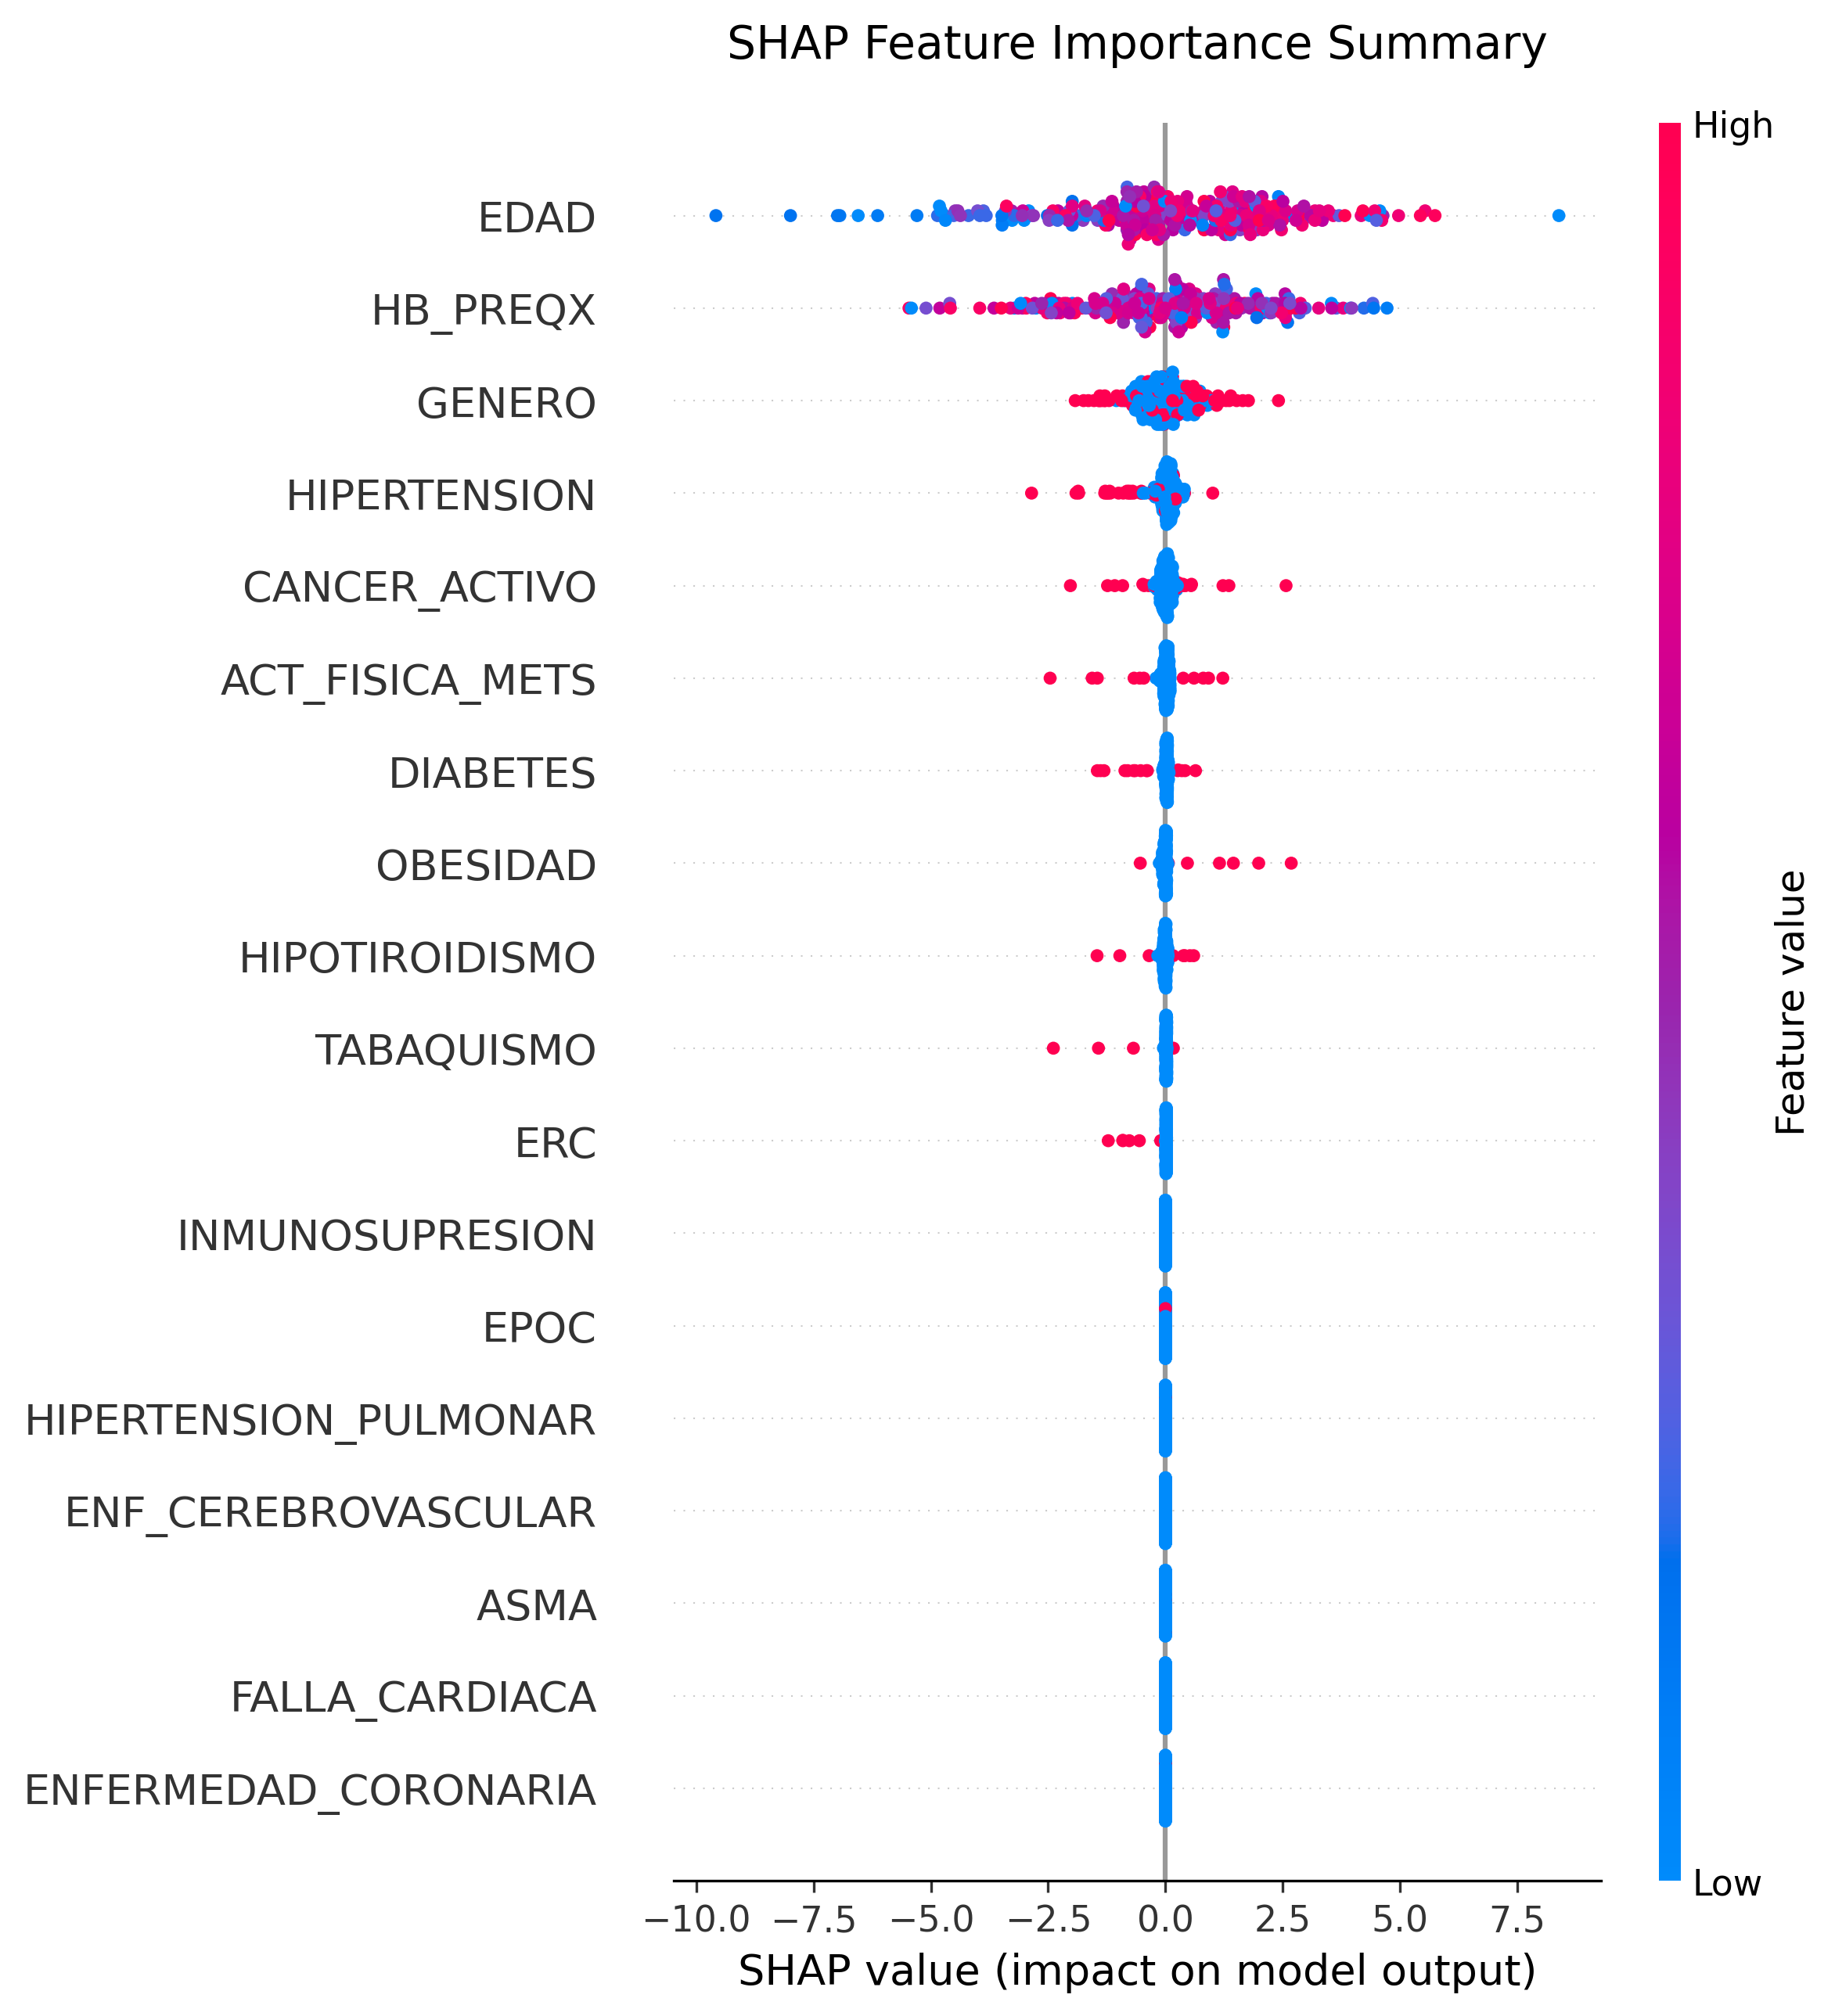
\includegraphics[width=0.85\textwidth]{images/exp_shap_summary.png}
\caption{Análisis SHAP de LightGBM mostrando la distribución de impacto de cada característica. EDAD y HB\_PREQX dominan las predicciones.}
\label{fig:shap-summary}
\end{figure}

\begin{figure}[H]
\centering
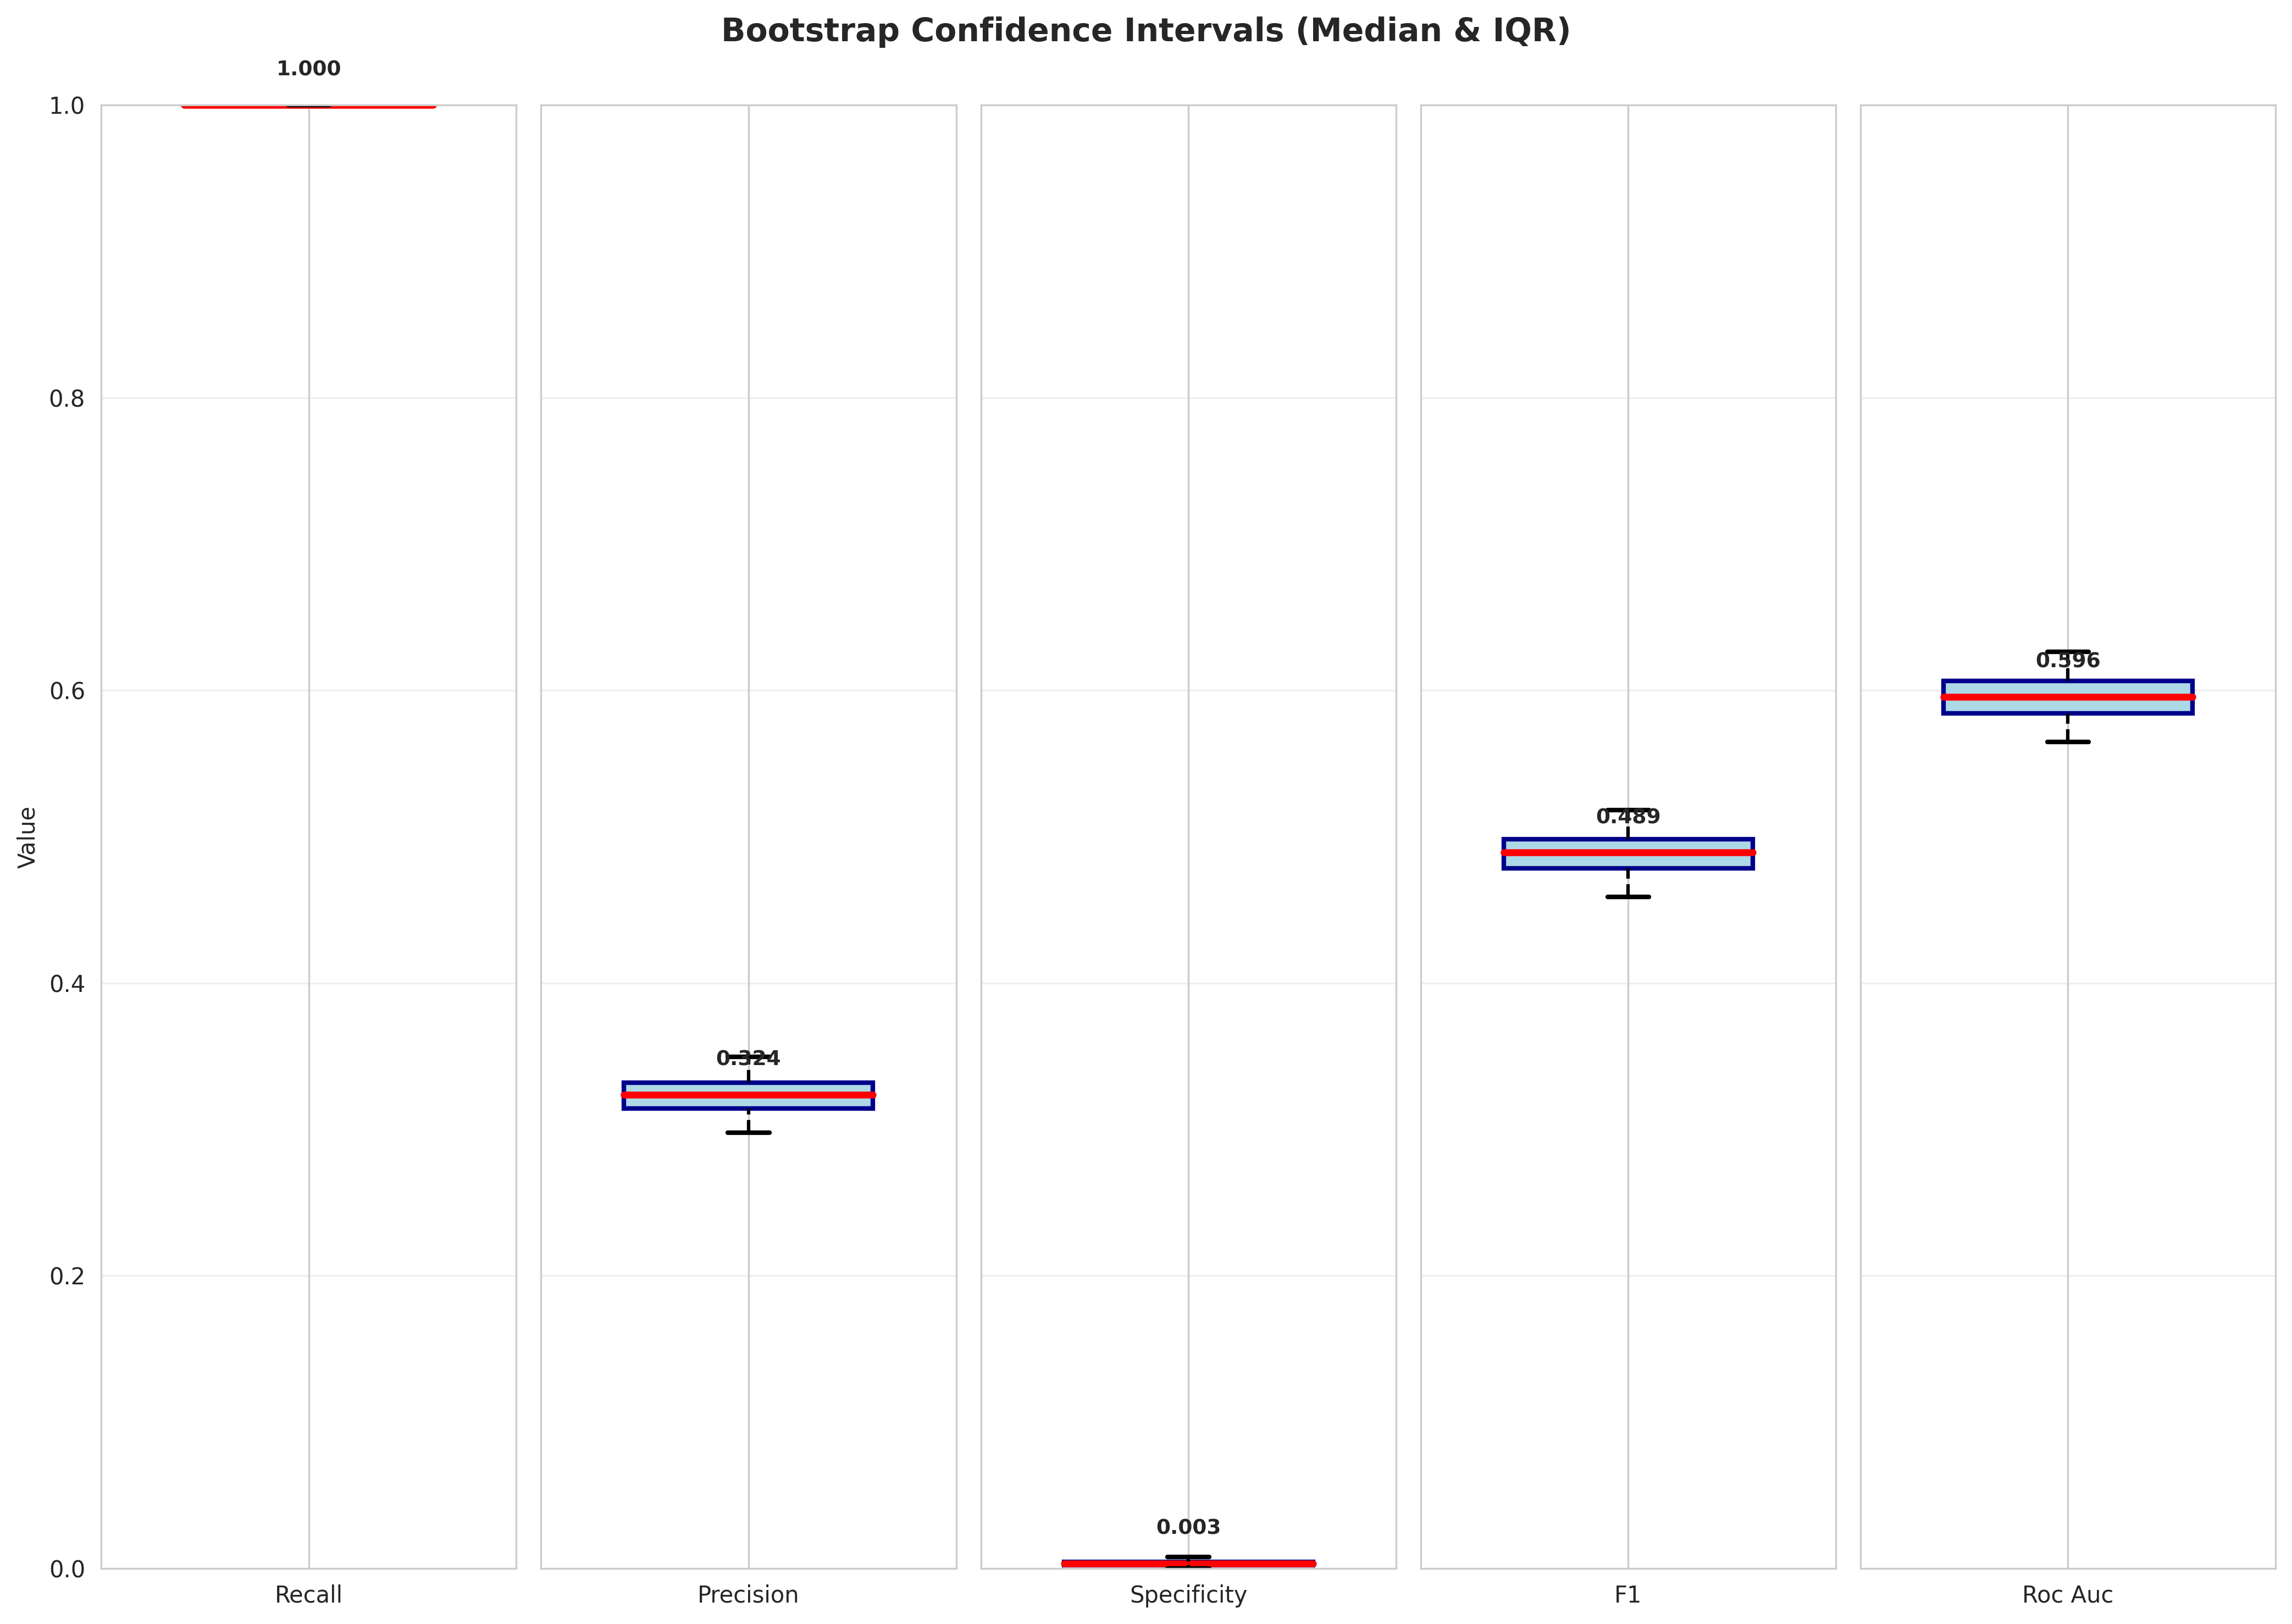
\includegraphics[width=0.85\textwidth]{images/exp_bootstrap.png}
\caption{Distribución bootstrap de métricas mostrando la variabilidad del rendimiento y los intervalos de confianza.}
\label{fig:bootstrap}
\end{figure}

\subsubsection{Análisis con reglas de asociación}

Se realizó un análisis de reglas de asociación utilizando el algoritmo Apriori para identificar patrones frecuentes entre las características y la variable objetivo. Este análisis permitió:

\begin{enumerate}
    \item Identificar combinaciones de características asociadas con mayor frecuencia al shock.
    \item Realizar selección de características basada en las reglas más significativas.
\end{enumerate}

Las reglas de asociación más relevantes identificadas fueron:

\begin{table}[H]
\centering
\caption{Principales reglas de asociación identificadas}
\label{tab:association-rules}
\small
\begin{tabular}{|p{6cm}|c|c|c|}
\hline
\textbf{Antecedente} & \textbf{Soporte} & \textbf{Confianza} & \textbf{Lift} \\ \hline
EDAD\_bin=3 \& HB\_PREQX\_bin=0 & 0.035 & 0.487 & 1.519 \\ \hline
HIPERTENSION=1 \& HIPOTIROIDISMO=1 & 0.011 & 0.414 & 1.291 \\ \hline
EDAD\_bin=2 \& HB\_PREQX\_bin=3 & 0.026 & 0.409 & 1.276 \\ \hline
EDAD\_bin=3 \& HB\_PREQX\_bin=2 & 0.026 & 0.409 & 1.276 \\ \hline
\end{tabular}
\end{table}

A partir de este análisis, se creó una versión del dataset con solo las características más relevantes según las reglas: EDAD, GENERO, HB\_PREQX, HIPERTENSION, DIABETES y CANCER\_ACTIVO.

\begin{table}[H]
\centering
\caption{Resultados con características seleccionadas por reglas de asociación}
\label{tab:exp-asociacion}
\begin{tabular}{|l|c|c|c|c|c|}
\hline
\textbf{Modelo} & \textbf{Recall} & \textbf{Precisión} & \textbf{Especificidad} & \textbf{F1-Score} & \textbf{AUC-ROC} \\ \hline
LightGBM & 0.238 & 0.241 & 0.646 & 0.240 & 0.509 \\ \hline
Gradient Boosting & 0.250 & 0.247 & 0.635 & 0.248 & 0.512 \\ \hline
Random Forest & 0.226 & 0.253 & 0.680 & 0.239 & 0.503 \\ \hline
\end{tabular}
\end{table}

La reducción de características no mejoró el rendimiento, confirmando que la información predictiva del dataset es limitada independientemente de la selección de variables.

\begin{figure}[H]
\centering
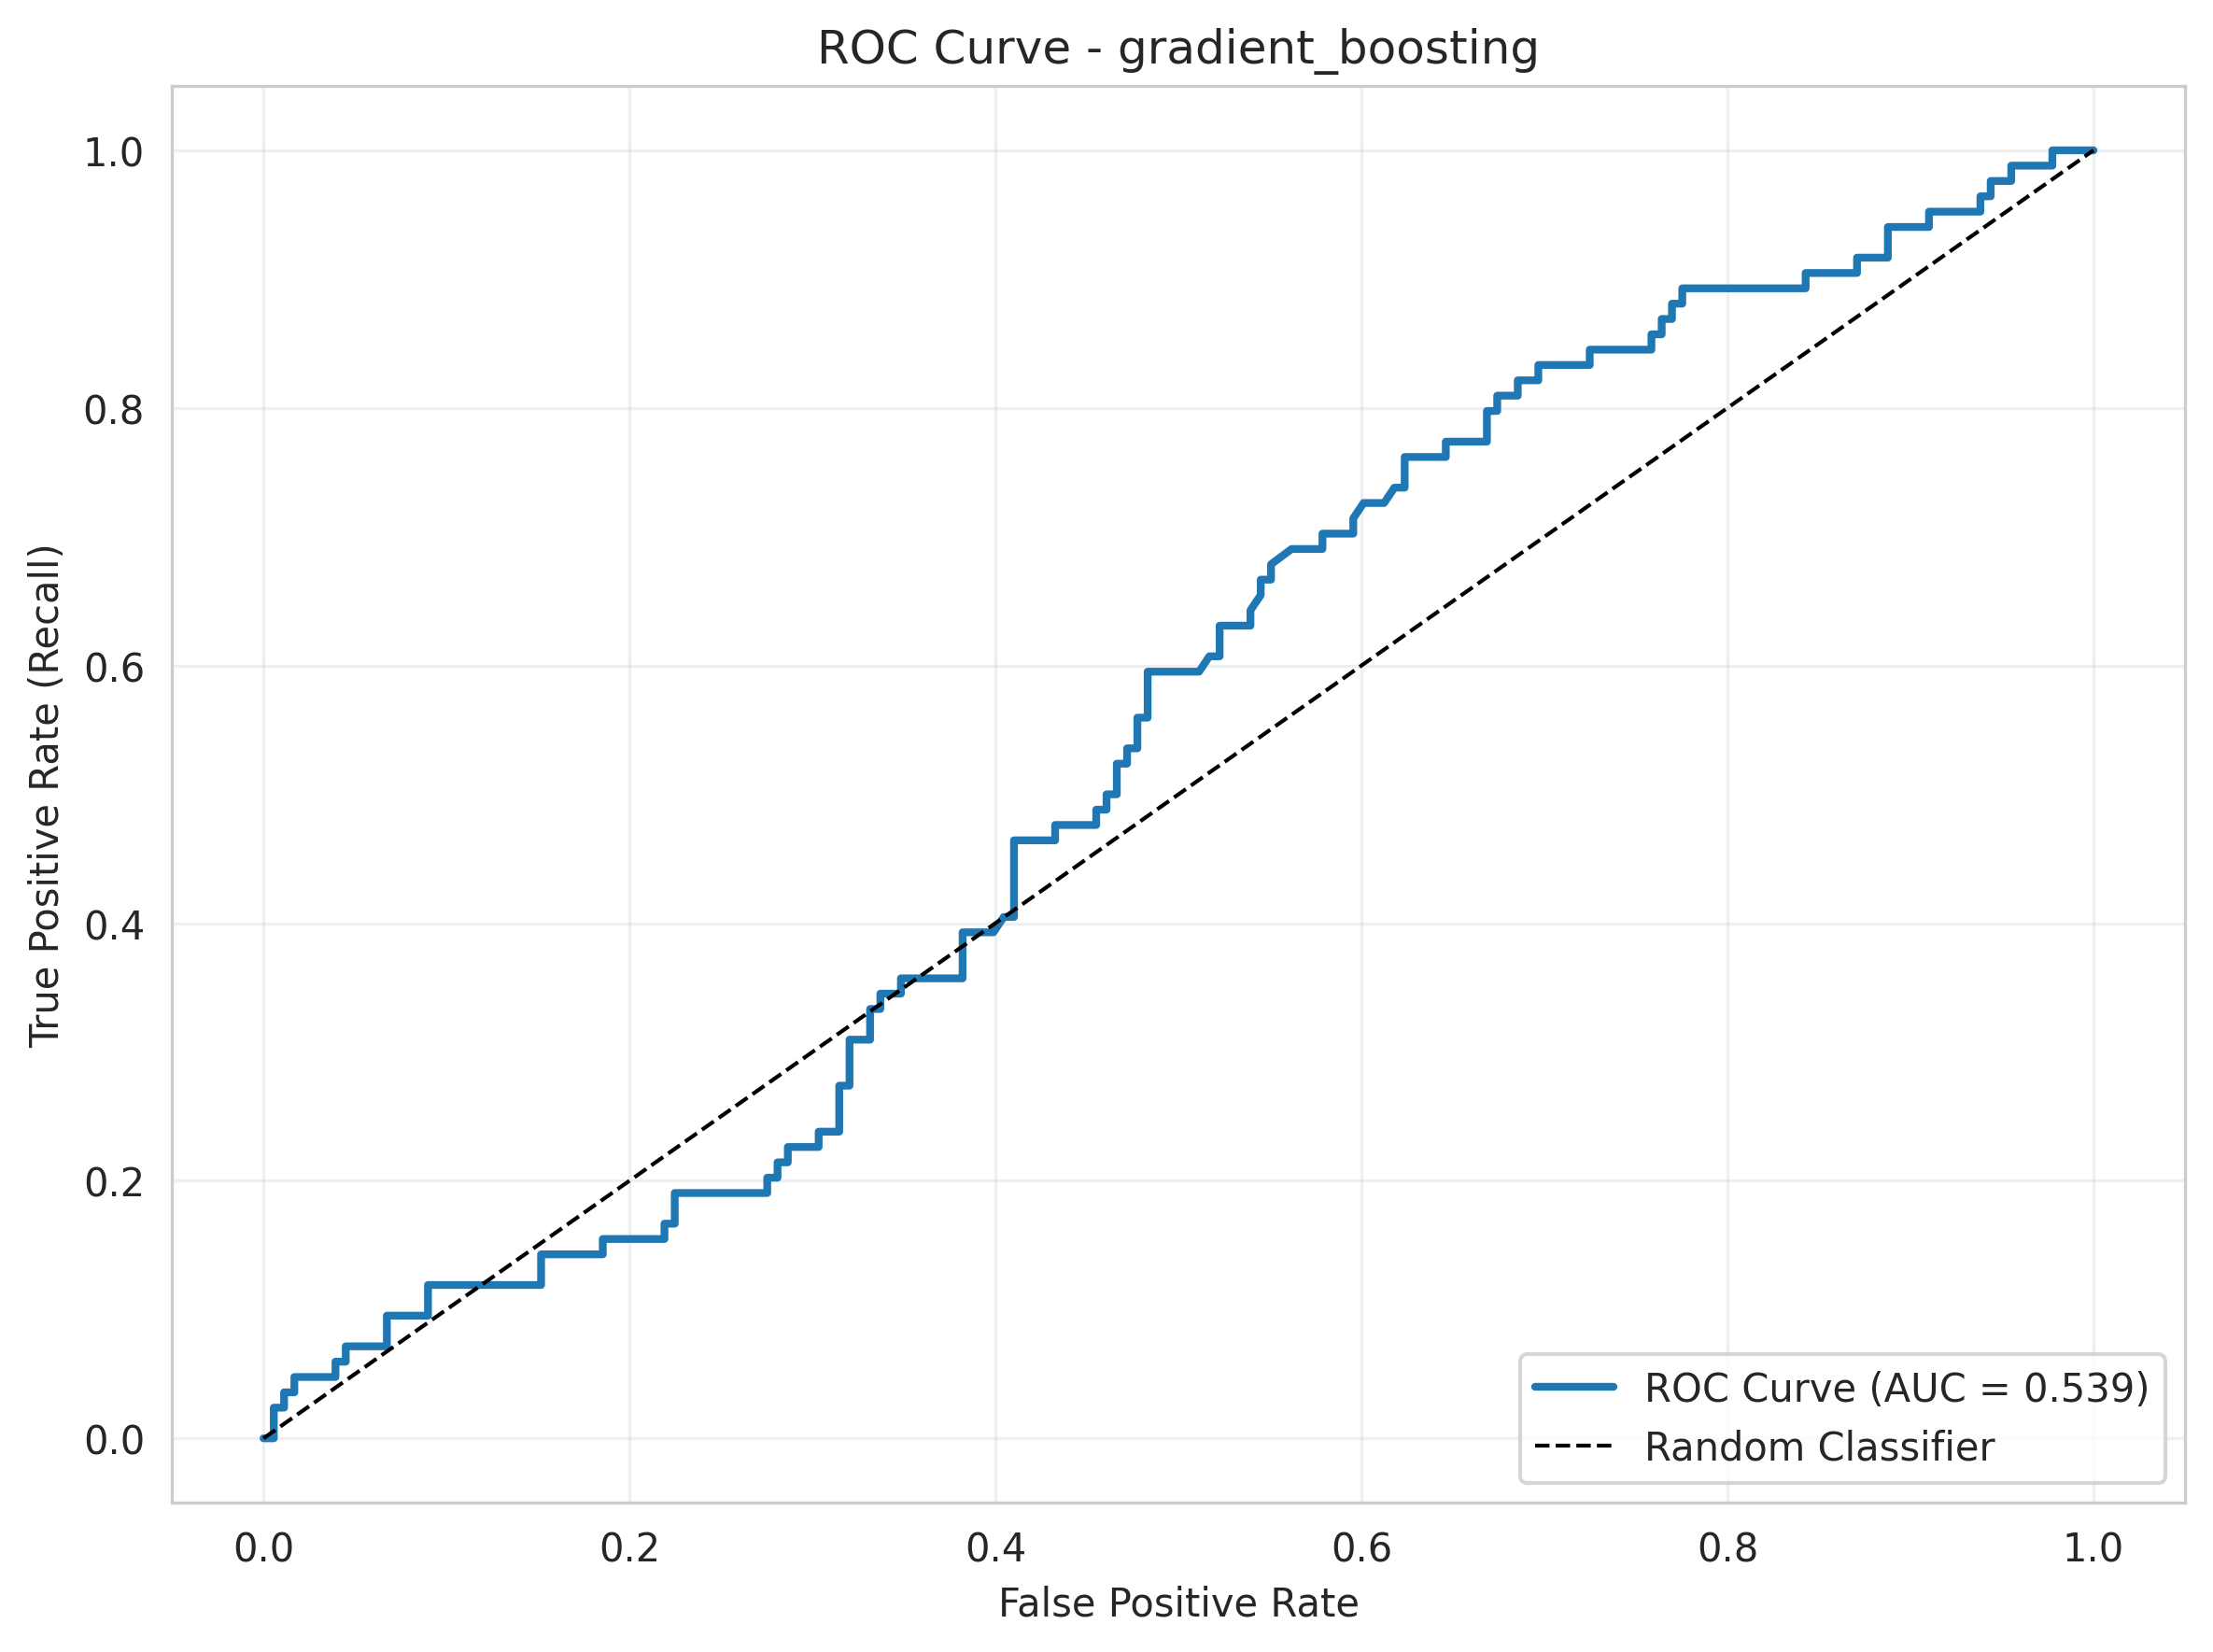
\includegraphics[width=0.8\textwidth]{images/exp_asociacion_roc.png}
\caption{Curva ROC con características seleccionadas por reglas de asociación (Gradient Boosting). AUC de 0.539.}
\label{fig:asociacion-roc}
\end{figure}

\subsubsection{Inclusión de variable intraoperatoria: SANGRADO\_MAYOR}

La variable SANGRADO\_MAYOR estaba presente en el dataset original, pero no había sido utilizada en los experimentos iniciales debido a su naturaleza intraoperatoria. Tras consultar con los especialistas médicos del equipo, se confirmó que esta variable se registra de forma casi inmediata al término de la cirugía, lo que la hace disponible para predicción temprana postoperatoria.

Es importante señalar que, contrario a lo esperado, el análisis inicial de Cramér's V mostró una correlación baja entre SANGRADO\_MAYOR y la variable objetivo. Sin embargo, los experimentos demostraron que su inclusión mejora sustancialmente el rendimiento predictivo de los modelos.

\begin{table}[H]
\centering
\caption{Resultados con SANGRADO\_MAYOR incluido}
\label{tab:exp-sangrado}
\begin{tabular}{|l|c|c|c|c|c|}
\hline
\textbf{Modelo} & \textbf{Recall} & \textbf{Precisión} & \textbf{Especificidad} & \textbf{F1-Score} & \textbf{AUC-ROC} \\ \hline
Decision Tree & 0.798 & 0.390 & 0.410 & 0.523 & 0.686 \\ \hline
LightGBM & 0.810 & 0.362 & 0.326 & 0.500 & 0.653 \\ \hline
\end{tabular}
\end{table}

La inclusión de SANGRADO\_MAYOR produjo una mejora notable en el rendimiento. El modelo LightGBM alcanzó un AUC-ROC de 0.653, superando consistentemente los resultados de experimentos anteriores que no incluían esta variable (AUC-ROC máximo previo: 0.58).

La evolución del rendimiento a lo largo de los experimentos se ilustra en las siguientes curvas ROC, que muestran la progresión desde el rendimiento inicial hasta la configuración final optimizada:

\begin{figure}[H]
\centering
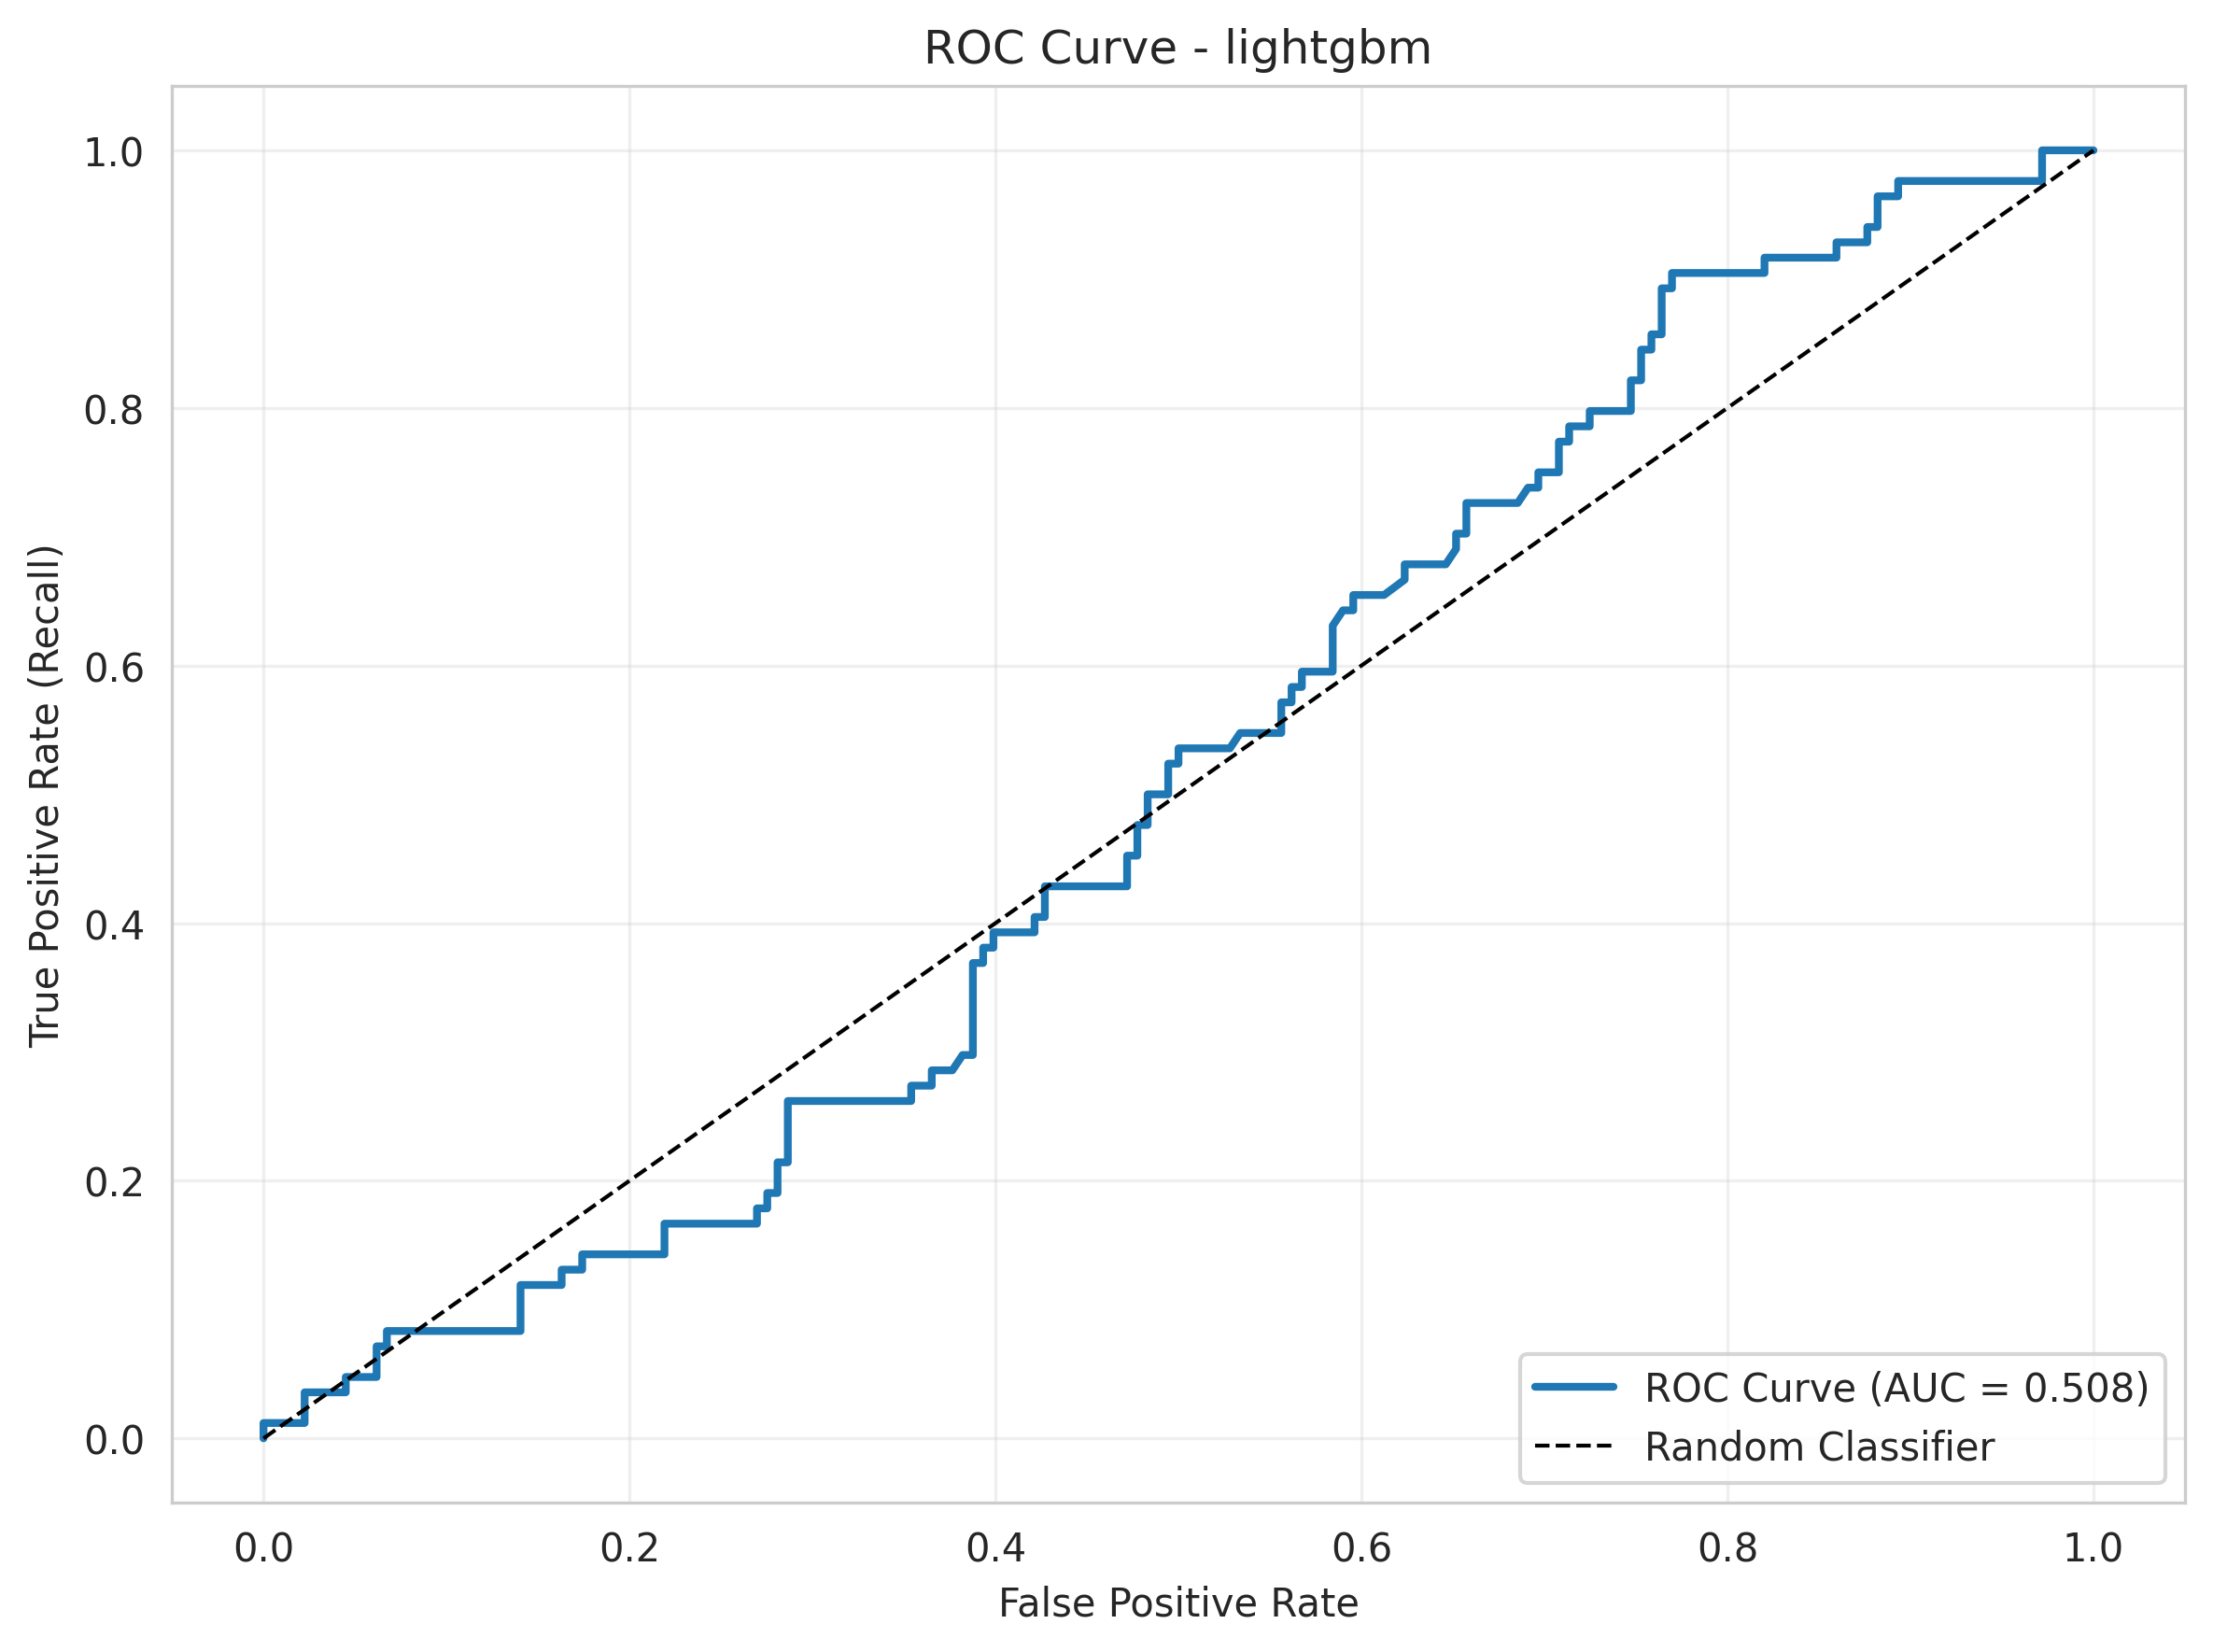
\includegraphics[width=0.8\textwidth]{images/exp_roc_v10.png}
\caption{Curva ROC inicial con nuevos modelos. LightGBM muestra AUC de 0.508, apenas superior al azar.}
\label{fig:roc-v10}
\end{figure}

\begin{figure}[H]
\centering
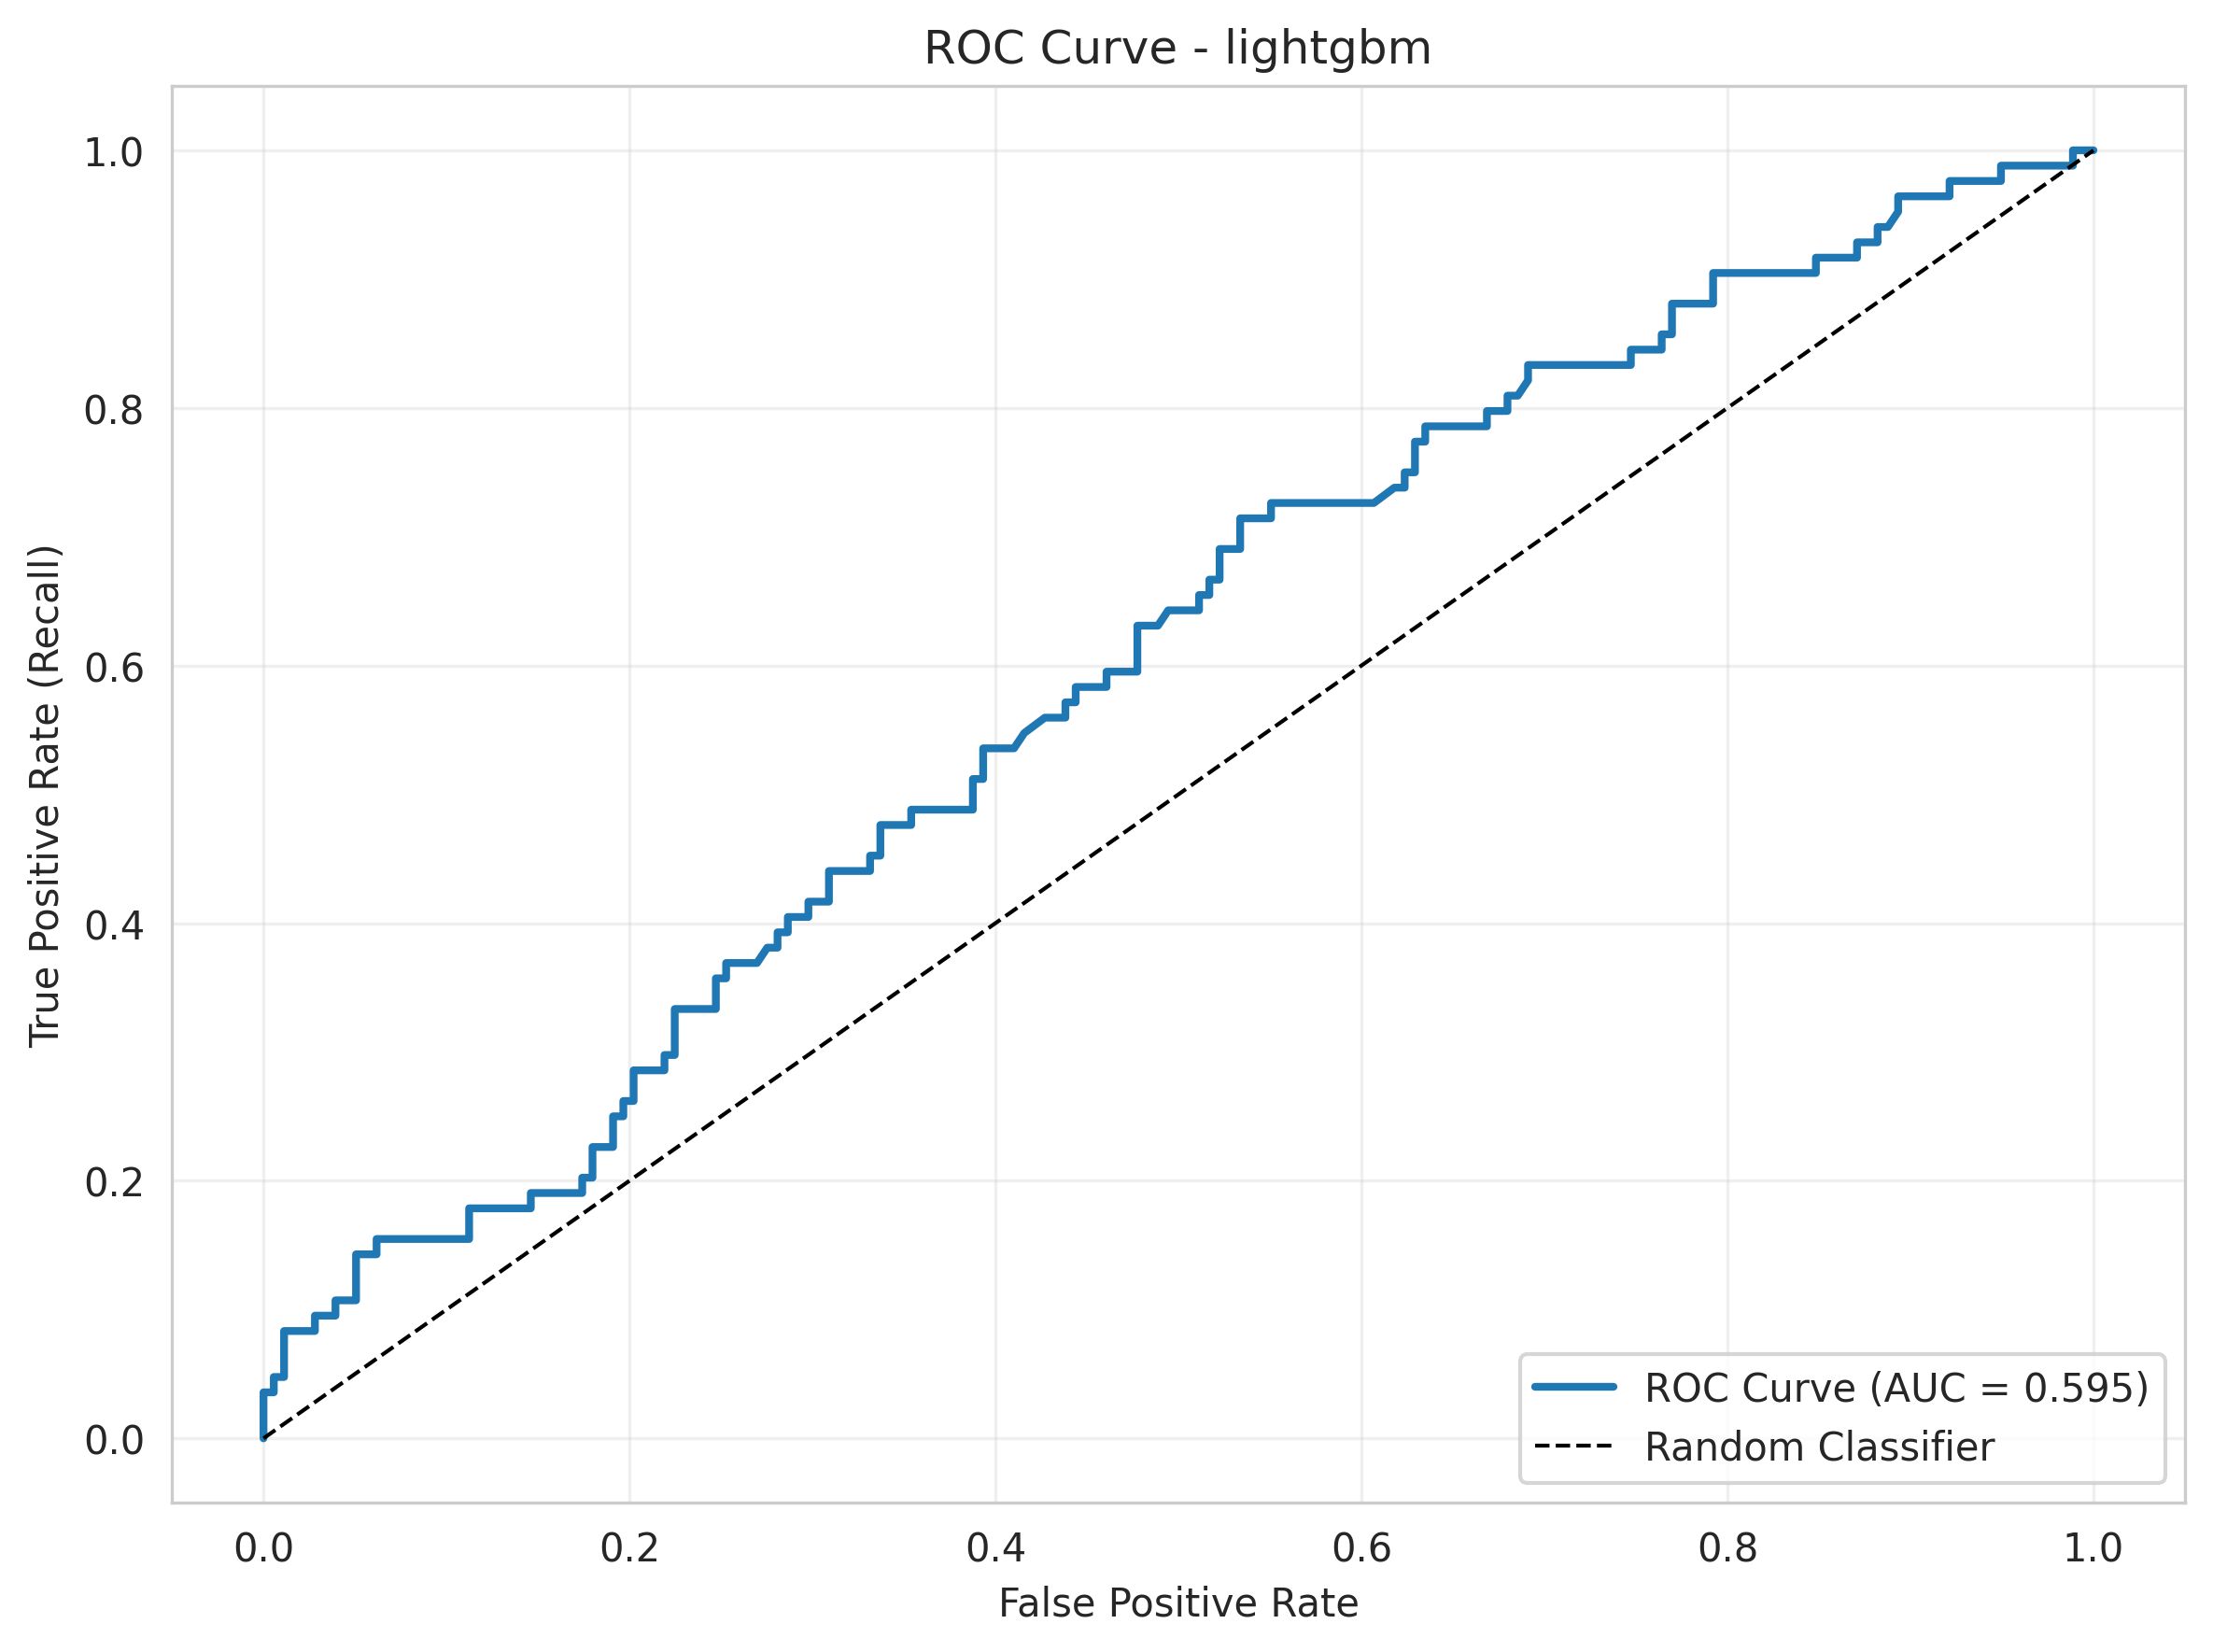
\includegraphics[width=0.8\textwidth]{images/exp_roc_v18.png}
\caption{Curva ROC tras optimización de hiperparámetros. LightGBM mejora a AUC de 0.595.}
\label{fig:roc-v18}
\end{figure}

\begin{figure}[H]
\centering
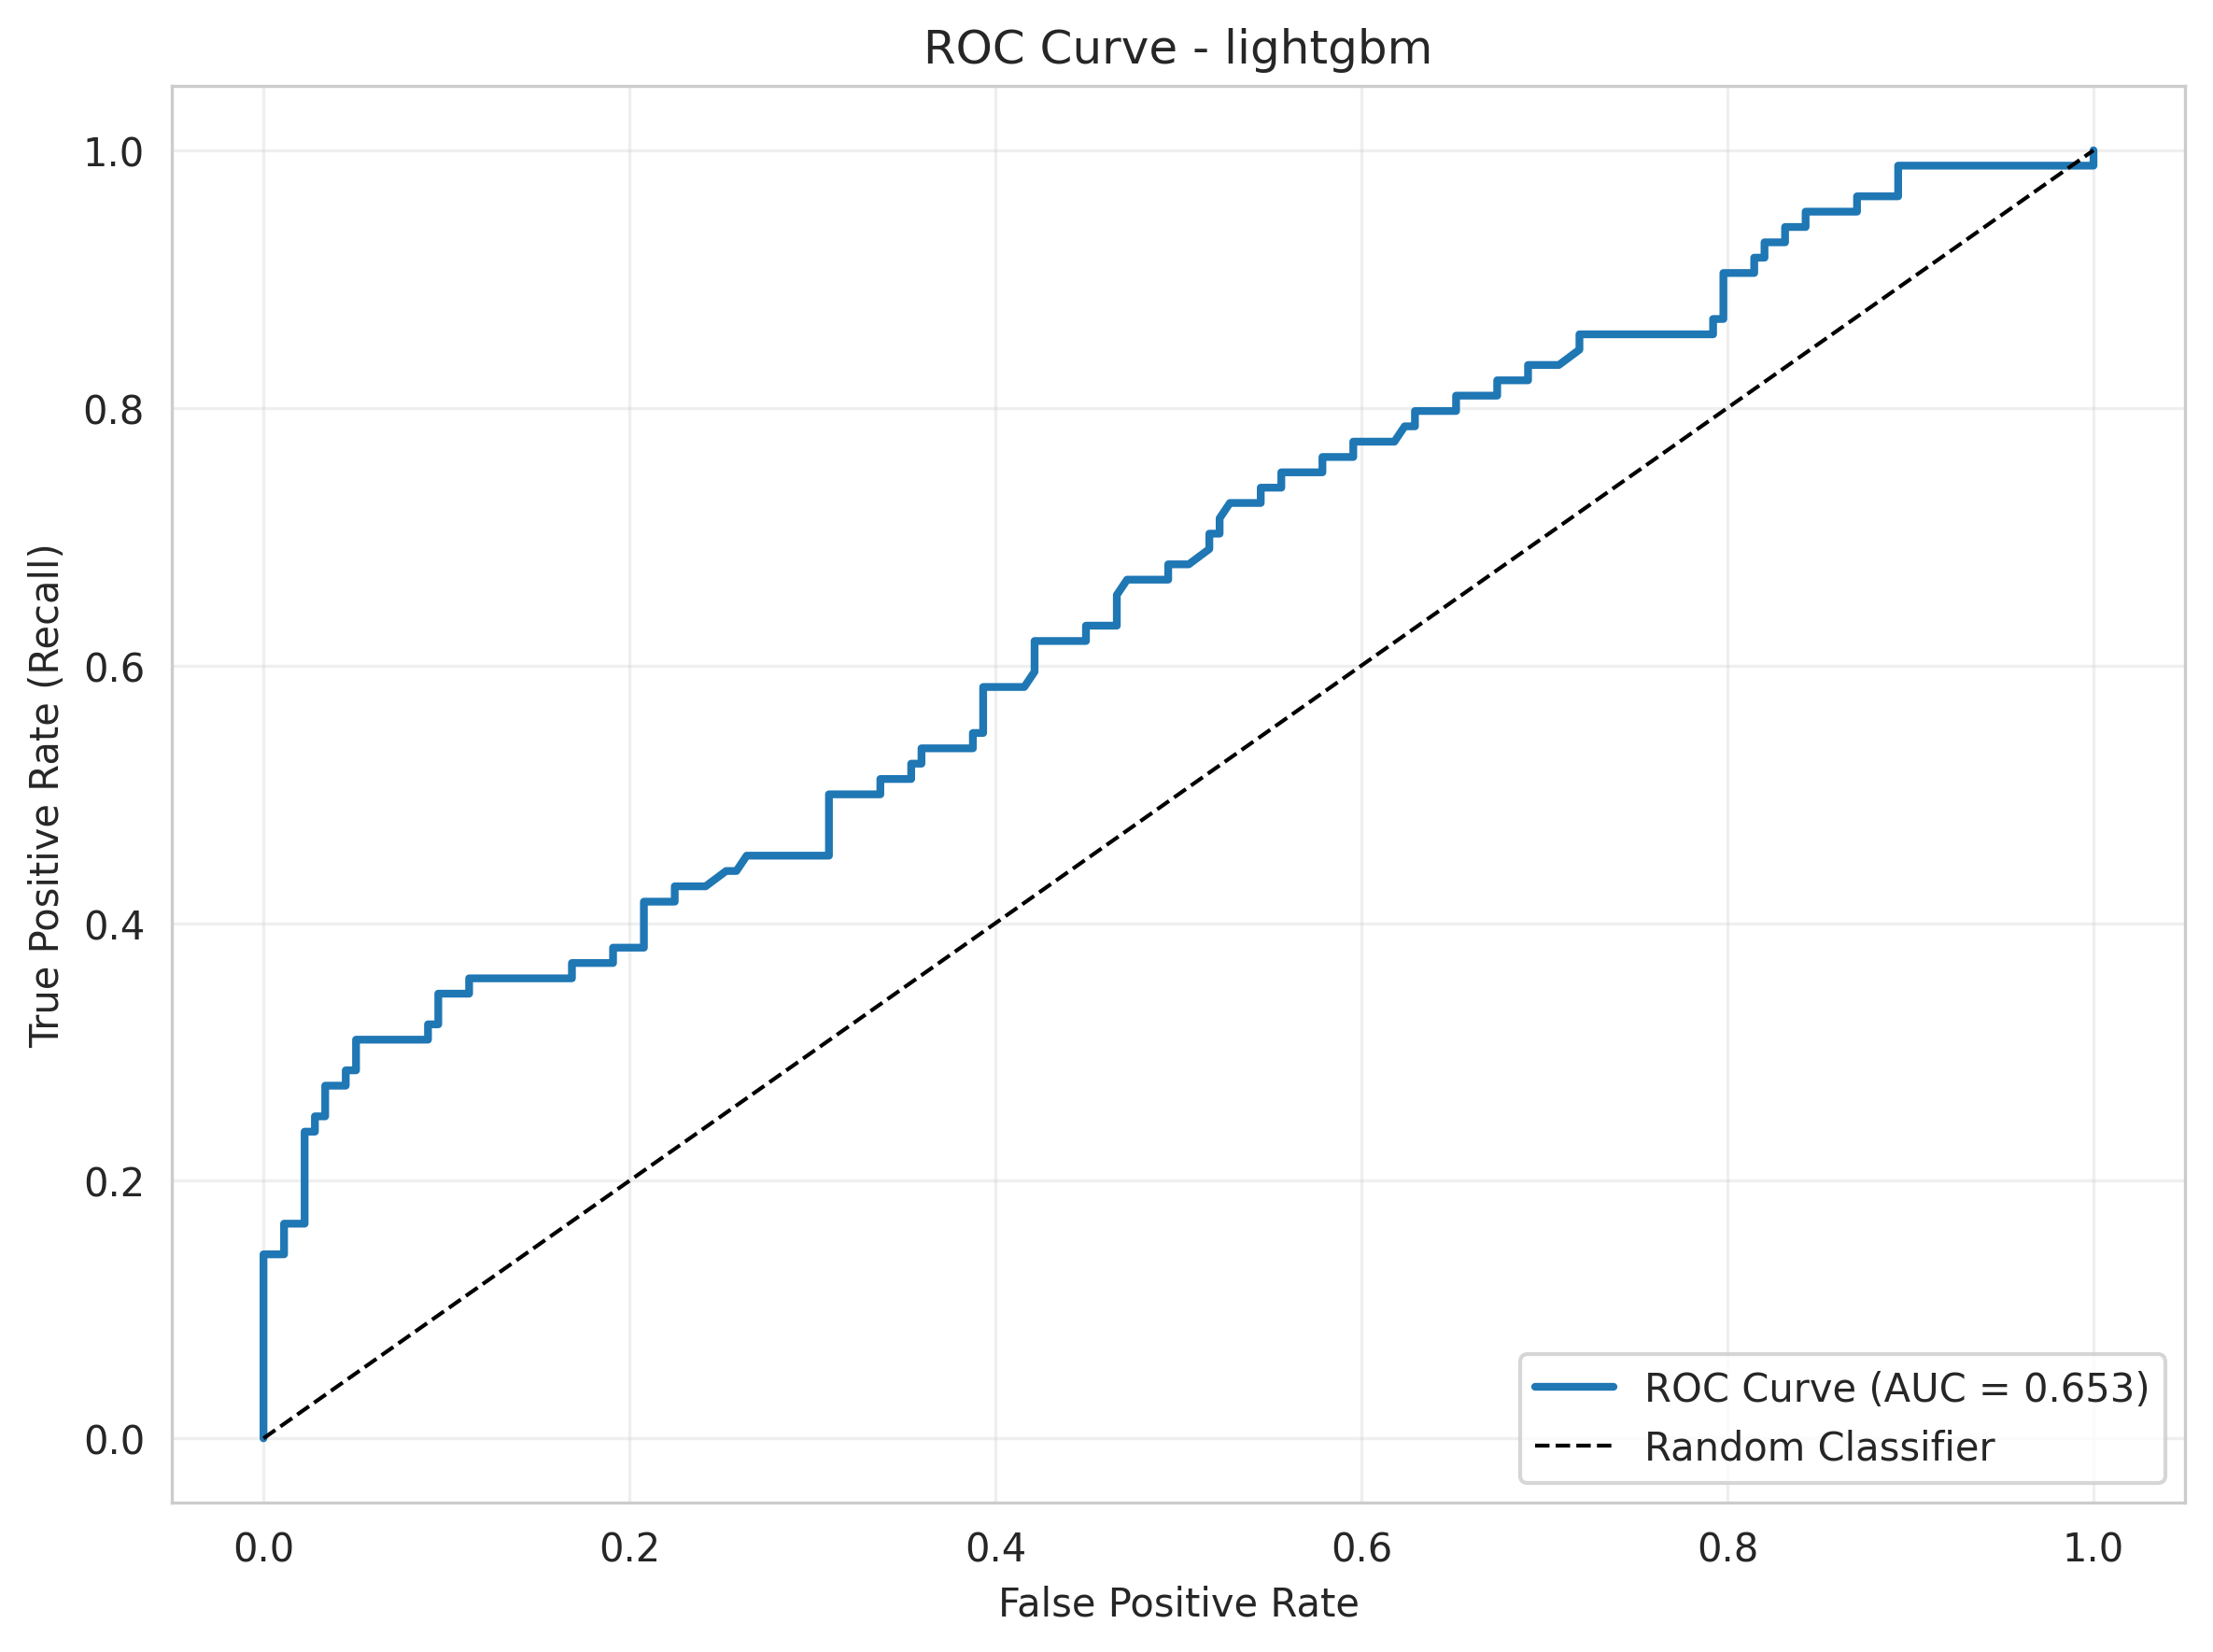
\includegraphics[width=0.8\textwidth]{images/exp_roc_v17.png}
\caption{Curva ROC con SANGRADO\_MAYOR incluido. LightGBM alcanza AUC de 0.653, el mejor resultado obtenido.}
\label{fig:roc-v17}
\end{figure}

\subsubsection{Comparación de LightGBM base versus umbral optimizado}

Con el fin de evaluar el impacto de la optimización del umbral de decisión sobre el rendimiento del modelo seleccionado, se comparan las métricas de validación cruzada del LightGBM base (umbral por defecto de 0.5) con las métricas obtenidas en el conjunto de prueba tras la optimización del umbral (0.54). Esta comparación permite cuantificar la ganancia clínica derivada del ajuste del punto de corte.

\begin{table}[H]
\centering
\caption{LightGBM: Validación cruzada (base) vs. umbral optimizado (prueba)}
\label{tab:exp-interpretables}
\footnotesize
\begin{tabular}{|p{4.5cm}|c|c|c|c|c|c|}
\hline
\textbf{Configuración} & \textbf{Recall} & \textbf{Prec.} & \textbf{Espec.} & \textbf{F1} & \textbf{AUC} & \textbf{Kappa} \\ \hline
LightGBM base (CV, umbral 0.5) & 0.904 & 0.349 & --- & 0.503 & 0.597 & 0.076 \\ \hline
LightGBM optimizado (prueba, 0.54) & 0.943 & 0.379 & 0.272 & 0.541 & 0.597 & 0.154 \\ \hline
\end{tabular}
\end{table}

La optimización del umbral mejoró el recall de 0.904 a 0.943 y el F1-Score de 0.503 a 0.541, con una ganancia también en Kappa (de 0.076 a 0.154), lo que indica una mayor concordancia con las etiquetas reales. La especificidad de 0.272 refleja la priorización de la sensibilidad en un contexto clínico donde la no detección de un caso de shock conlleva consecuencias potencialmente fatales. Como señalan \cite{steyerberg2018}, los modelos pueden presentar resultados moderados en validación cruzada pero mostrar mejoras tangibles en el conjunto de prueba cuando se aplica una estrategia de optimización de umbral orientada al contexto clínico.

\textbf{Hiperparámetros óptimos del modelo LightGBM:}

\begin{itemize}
    \item \textbf{LightGBM:} n\_estimators=200, learning\_rate=0.03, num\_leaves=63, max\_depth=5, scale\_pos\_weight=3.0.
\end{itemize}

\begin{figure}[H]
\centering
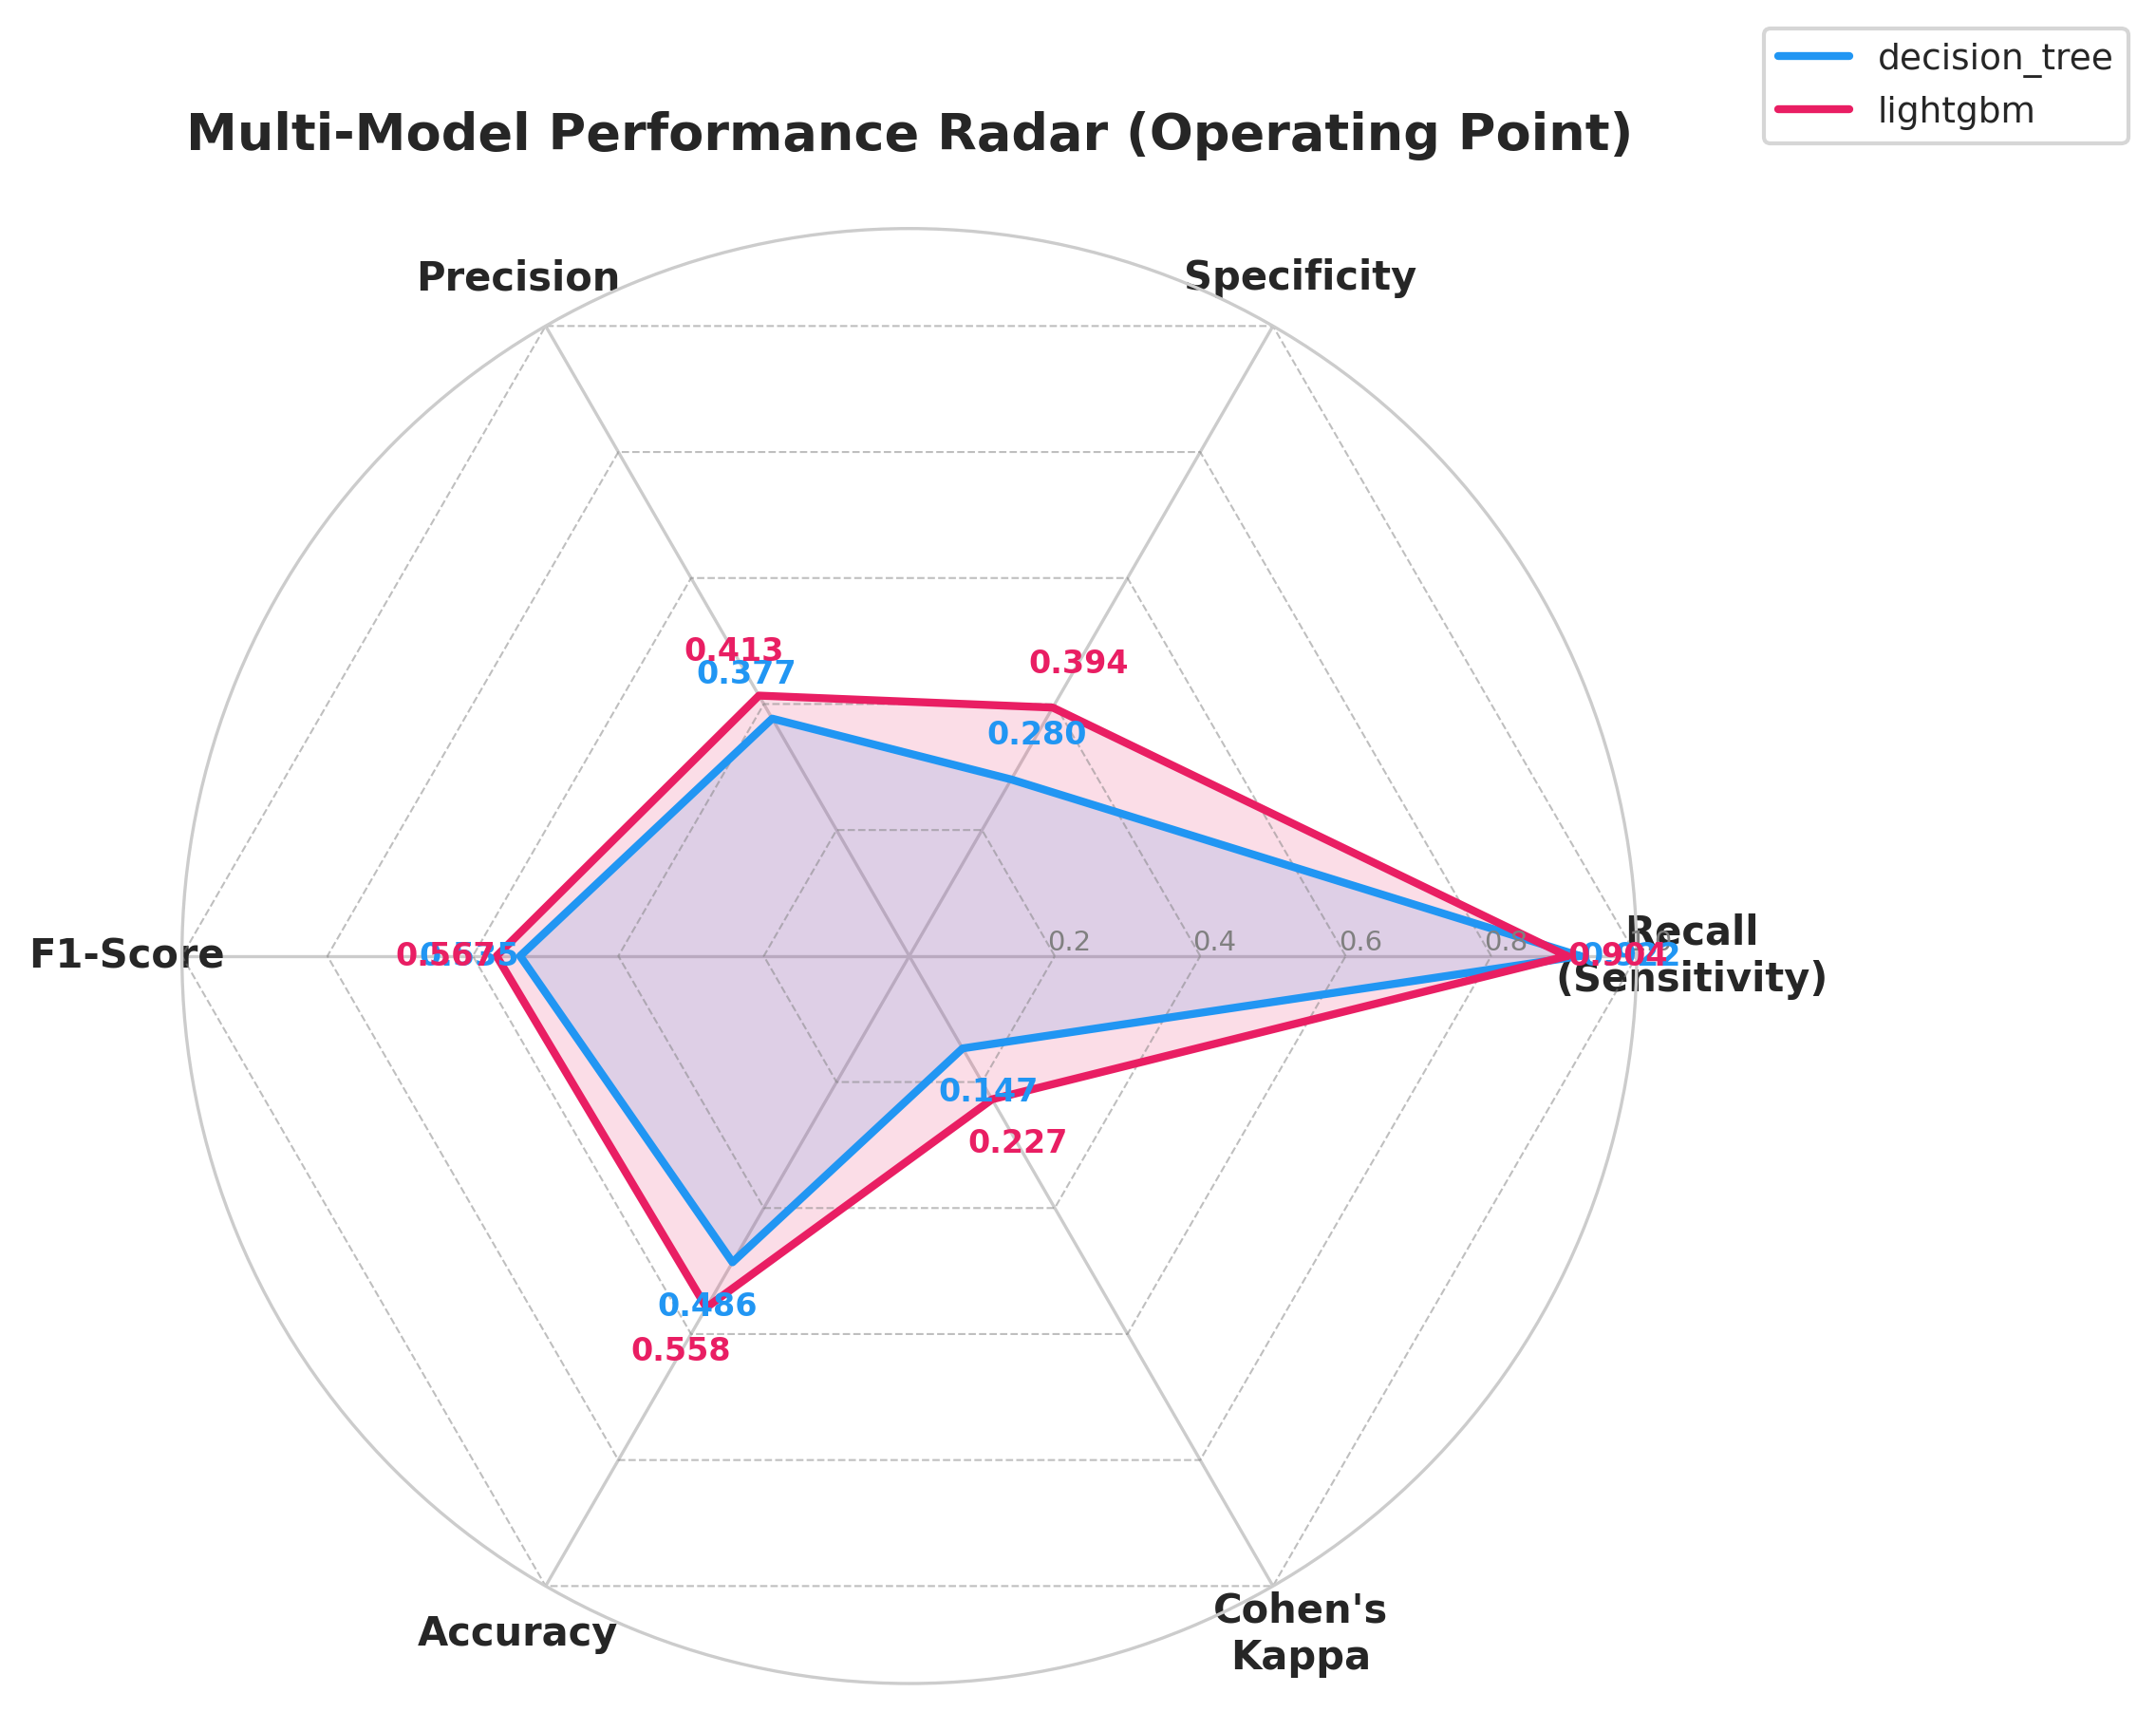
\includegraphics[width=0.85\textwidth]{images/exp_multimodel_radar.png}
\caption{Comparación radar de métricas entre modelos. Se observa el trade-off entre recall y especificidad en cada modelo.}
\label{fig:multimodel-radar}
\end{figure}

\begin{figure}[H]
\centering
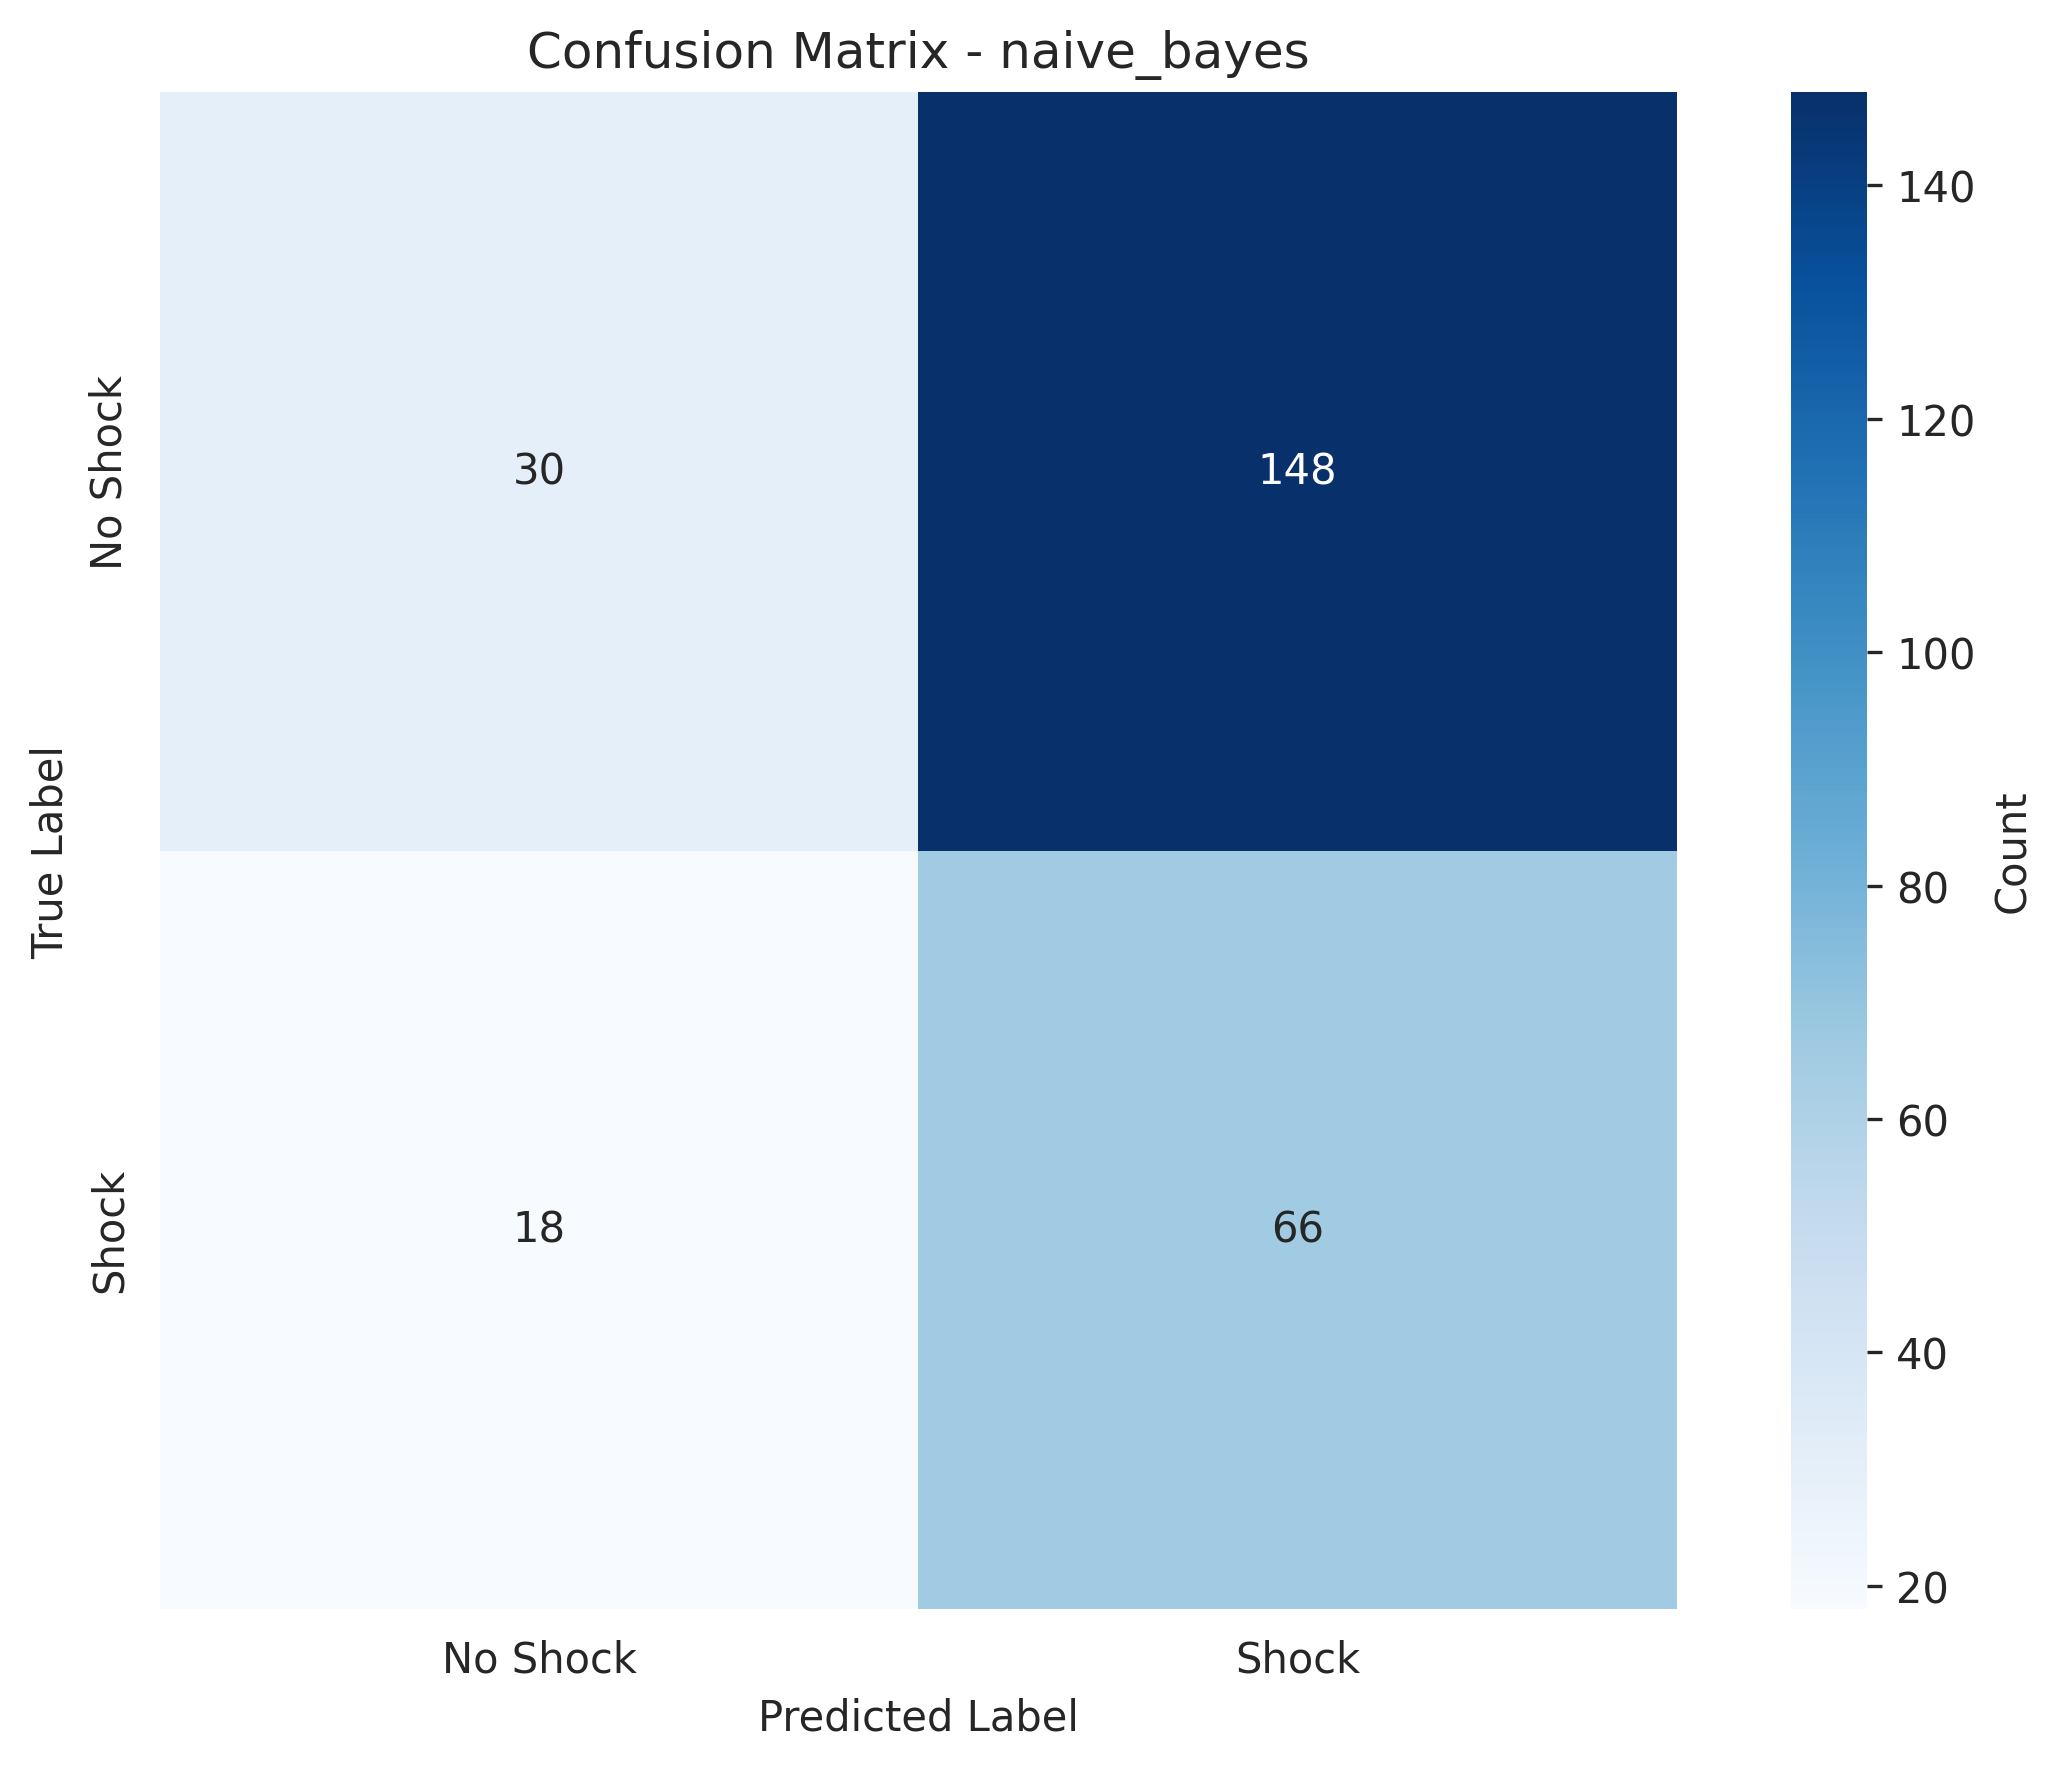
\includegraphics[width=0.65\textwidth]{images/exp_nb_confusion.png}
\caption{Matriz de confusión de Naive Bayes mostrando su tendencia a maximizar recall a costa de especificidad.}
\label{fig:nb-confusion}
\end{figure}

\subsubsection{Análisis de interpretabilidad con SHAP}

Se aplicó el método SHAP (SHapley Additive exPlanations) para cuantificar la contribución de cada característica a las predicciones del modelo. Este análisis se realizó principalmente sobre LightGBM debido a su mejor rendimiento.

\begin{table}[H]
\centering
\caption{Importancia de características según valores SHAP (LightGBM)}
\label{tab:shap-importance}
\begin{tabular}{|l|c|c|}
\hline
\textbf{Característica} & \textbf{Importancia SHAP} & \textbf{Importancia normalizada} \\ \hline
EDAD & 1.921 & 42.85\% \\ \hline
HB\_PREQX & 1.469 & 32.77\% \\ \hline
GENERO & 0.448 & 10.00\% \\ \hline
HIPERTENSION & 0.199 & 4.44\% \\ \hline
CANCER\_ACTIVO & 0.129 & 2.87\% \\ \hline
ACT\_FISICA\_METS & 0.083 & 1.85\% \\ \hline
DIABETES & 0.067 & 1.50\% \\ \hline
OBESIDAD & 0.055 & 1.24\% \\ \hline
\end{tabular}
\end{table}

El análisis SHAP reveló que EDAD y HB\_PREQX (hemoglobina prequirúrgica) son las características más influyentes, concentrando el 75.62\% de la importancia total. Esto es clínicamente coherente, ya que:

\begin{itemize}
    \item Los pacientes de mayor edad tienen menor capacidad de compensación hemodinámica.
    \item Niveles bajos de hemoglobina prequirúrgica indican menor reserva para tolerar pérdidas sanguíneas.
\end{itemize}

Las comorbilidades individuales tienen contribuciones marginales, lo que explica por qué las agregaciones de comorbilidades no mejoraron significativamente el rendimiento.

\subsubsection{Análisis de umbral de decisión}

Se realizó un análisis de umbrales para optimizar el punto de corte de clasificación según criterios clínicos. Dado que la consecuencia de no detectar un shock (falso negativo) es potencialmente fatal, se priorizó la maximización del recall manteniendo una especificidad razonable.

\begin{table}[H]
\centering
\caption{Análisis de umbrales de decisión para optimización clínica}
\label{tab:threshold-analysis}
\small
\begin{tabular}{|c|c|c|c|c|c|}
\hline
\textbf{Umbral} & \textbf{Recall} & \textbf{Precisión} & \textbf{Especificidad} & \textbf{F1-Score} & \textbf{F2-Score} \\ \hline
0.25 & 0.988 & 0.328 & 0.045 & 0.493 & 0.705 \\ \hline
0.30 & 0.964 & 0.336 & 0.101 & 0.498 & 0.702 \\ \hline
0.35 & 0.917 & 0.332 & 0.129 & 0.487 & 0.678 \\ \hline
0.40 & 0.881 & 0.344 & 0.208 & 0.495 & 0.672 \\ \hline
0.45 & 0.833 & 0.357 & 0.292 & 0.500 & 0.658 \\ \hline
\textbf{0.49} & \textbf{0.798} & \textbf{0.356} & \textbf{0.320} & \textbf{0.493} & \textbf{0.639} \\ \hline
0.50 & 0.798 & 0.360 & 0.331 & 0.496 & 0.642 \\ \hline
\end{tabular}
\end{table}

El umbral óptimo identificado fue 0.49, que ofrece un recall de 79.8\% con una especificidad de 32.0\%. Aunque la especificidad es baja, en el contexto clínico es preferible generar falsas alarmas (que pueden ser descartadas por el equipo médico) a no detectar casos de shock potencialmente fatales.

\subsubsection{Resumen comparativo de experimentos}

\begin{table}[H]
\centering
\caption{Resumen comparativo de los principales experimentos}
\label{tab:summary-experiments}
\small
\begin{tabular}{|p{4.5cm}|c|c|p{4cm}|}
\hline
\textbf{Experimento} & \textbf{Mejor AUC-ROC} & \textbf{Mejor Modelo} & \textbf{Observación} \\ \hline
Dataset base & 0.580 & Reg. Logística & Línea base \\ \hline
Categorización & 0.578 & Reg. Logística & Sin mejora \\ \hline
Agregaciones & 0.573 & Reg. Logística & Sin mejora \\ \hline
Combinado & 0.571 & Reg. Logística & Sin mejora \\ \hline
Ajuste de hiperparámetros & 0.560 & Gradient Boosting & Mejora marginal \\ \hline
Nuevos modelos & 0.508 & LightGBM & Rendimiento inicial bajo \\ \hline
Reglas de asociación & 0.512 & Gradient Boosting & Rendimiento inferior \\ \hline
SANGRADO\_MAYOR + optimización & 0.653 & LightGBM & \textbf{Mejor resultado} \\ \hline
Modelos interpretables & 0.606 & Decision Tree & Balance interpretable \\ \hline
\end{tabular}
\end{table}

\subsubsection{Discusión de resultados experimentales}

Los experimentos realizados permiten extraer las siguientes conclusiones:

\begin{enumerate}
    \item \textbf{Limitación de características preoperatorias:} Las características preoperatorias disponibles (comorbilidades, datos demográficos, hemoglobina) tienen capacidad predictiva limitada para el shock hemorrágico. El AUC-ROC máximo alcanzado sin SANGRADO\_MAYOR fue de 0.58, apenas superior al azar.
    
    \item \textbf{Importancia de variables intraoperatorias:} La inclusión de SANGRADO\_MAYOR elevó el AUC-ROC a 0.653, demostrando que la información intraoperatoria es fundamental para la predicción temprana del shock.
    
    \item \textbf{Ingeniería de características insuficiente:} Ni la categorización de variables continuas ni las agregaciones de comorbilidades mejoraron el rendimiento predictivo. Las características derivadas introducen redundancia sin aportar información discriminativa adicional.
    
    \item \textbf{Relevancia de EDAD y HB\_PREQX:} El análisis SHAP confirmó que estas dos variables concentran más del 75\% de la importancia predictiva, lo que es clínicamente coherente con los mecanismos fisiopatológicos del shock.
    
    \item \textbf{Trade-off entre recall y especificidad:} En el contexto clínico, se prefiere un modelo con alto recall (baja tasa de falsos negativos) aunque esto implique menor especificidad. Un caso de shock no detectado puede ser fatal, mientras que una falsa alarma puede ser descartada por el equipo médico.
    
    \item \textbf{Modelos interpretables viables:} Decision Tree ofrece un balance aceptable entre rendimiento y explicabilidad, facilitando su adopción en entornos clínicos donde la transparencia del modelo es requisito.
\end{enumerate}

\subsubsection{Modelo seleccionado y configuración final}

Tras el análisis exhaustivo de todos los experimentos, se seleccionó \textbf{LightGBM} como el modelo óptimo para la predicción del shock hemorrágico, obtenido en el experimento con inclusión de SANGRADO\_MAYOR y optimización de hiperparámetros.

\textbf{Rendimiento del modelo seleccionado:}

\begin{table}[H]
\centering
\caption{Métricas del modelo LightGBM seleccionado}
\label{tab:modelo-final}
\begin{tabular}{|l|c|}
\hline
\textbf{Métrica} & \textbf{Valor} \\ \hline
AUC-ROC & 0.653 \\ \hline
Recall & 0.810 \\ \hline
Precisión & 0.362 \\ \hline
Especificidad & 0.326 \\ \hline
F1-Score & 0.500 \\ \hline
\end{tabular}
\end{table}

\textbf{Hiperparámetros óptimos:}

\begin{itemize}
    \item \texttt{n\_estimators}: 200
    \item \texttt{learning\_rate}: 0.03
    \item \texttt{num\_leaves}: 63
    \item \texttt{max\_depth}: 5
    \item \texttt{scale\_pos\_weight}: 3.0 (para manejo de desbalance)
    \item \texttt{min\_child\_samples}: 20
\end{itemize}

\textbf{Umbral de decisión óptimo:} 0.49, seleccionado para maximizar recall en contexto clínico.

\textbf{Características utilizadas:} EDAD, HB\_PREQX, GENERO, SANGRADO\_MAYOR, HIPERTENSION, CANCER\_ACTIVO, ACT\_FISICA\_METS, DIABETES, OBESIDAD.

\begin{figure}[H]
\centering
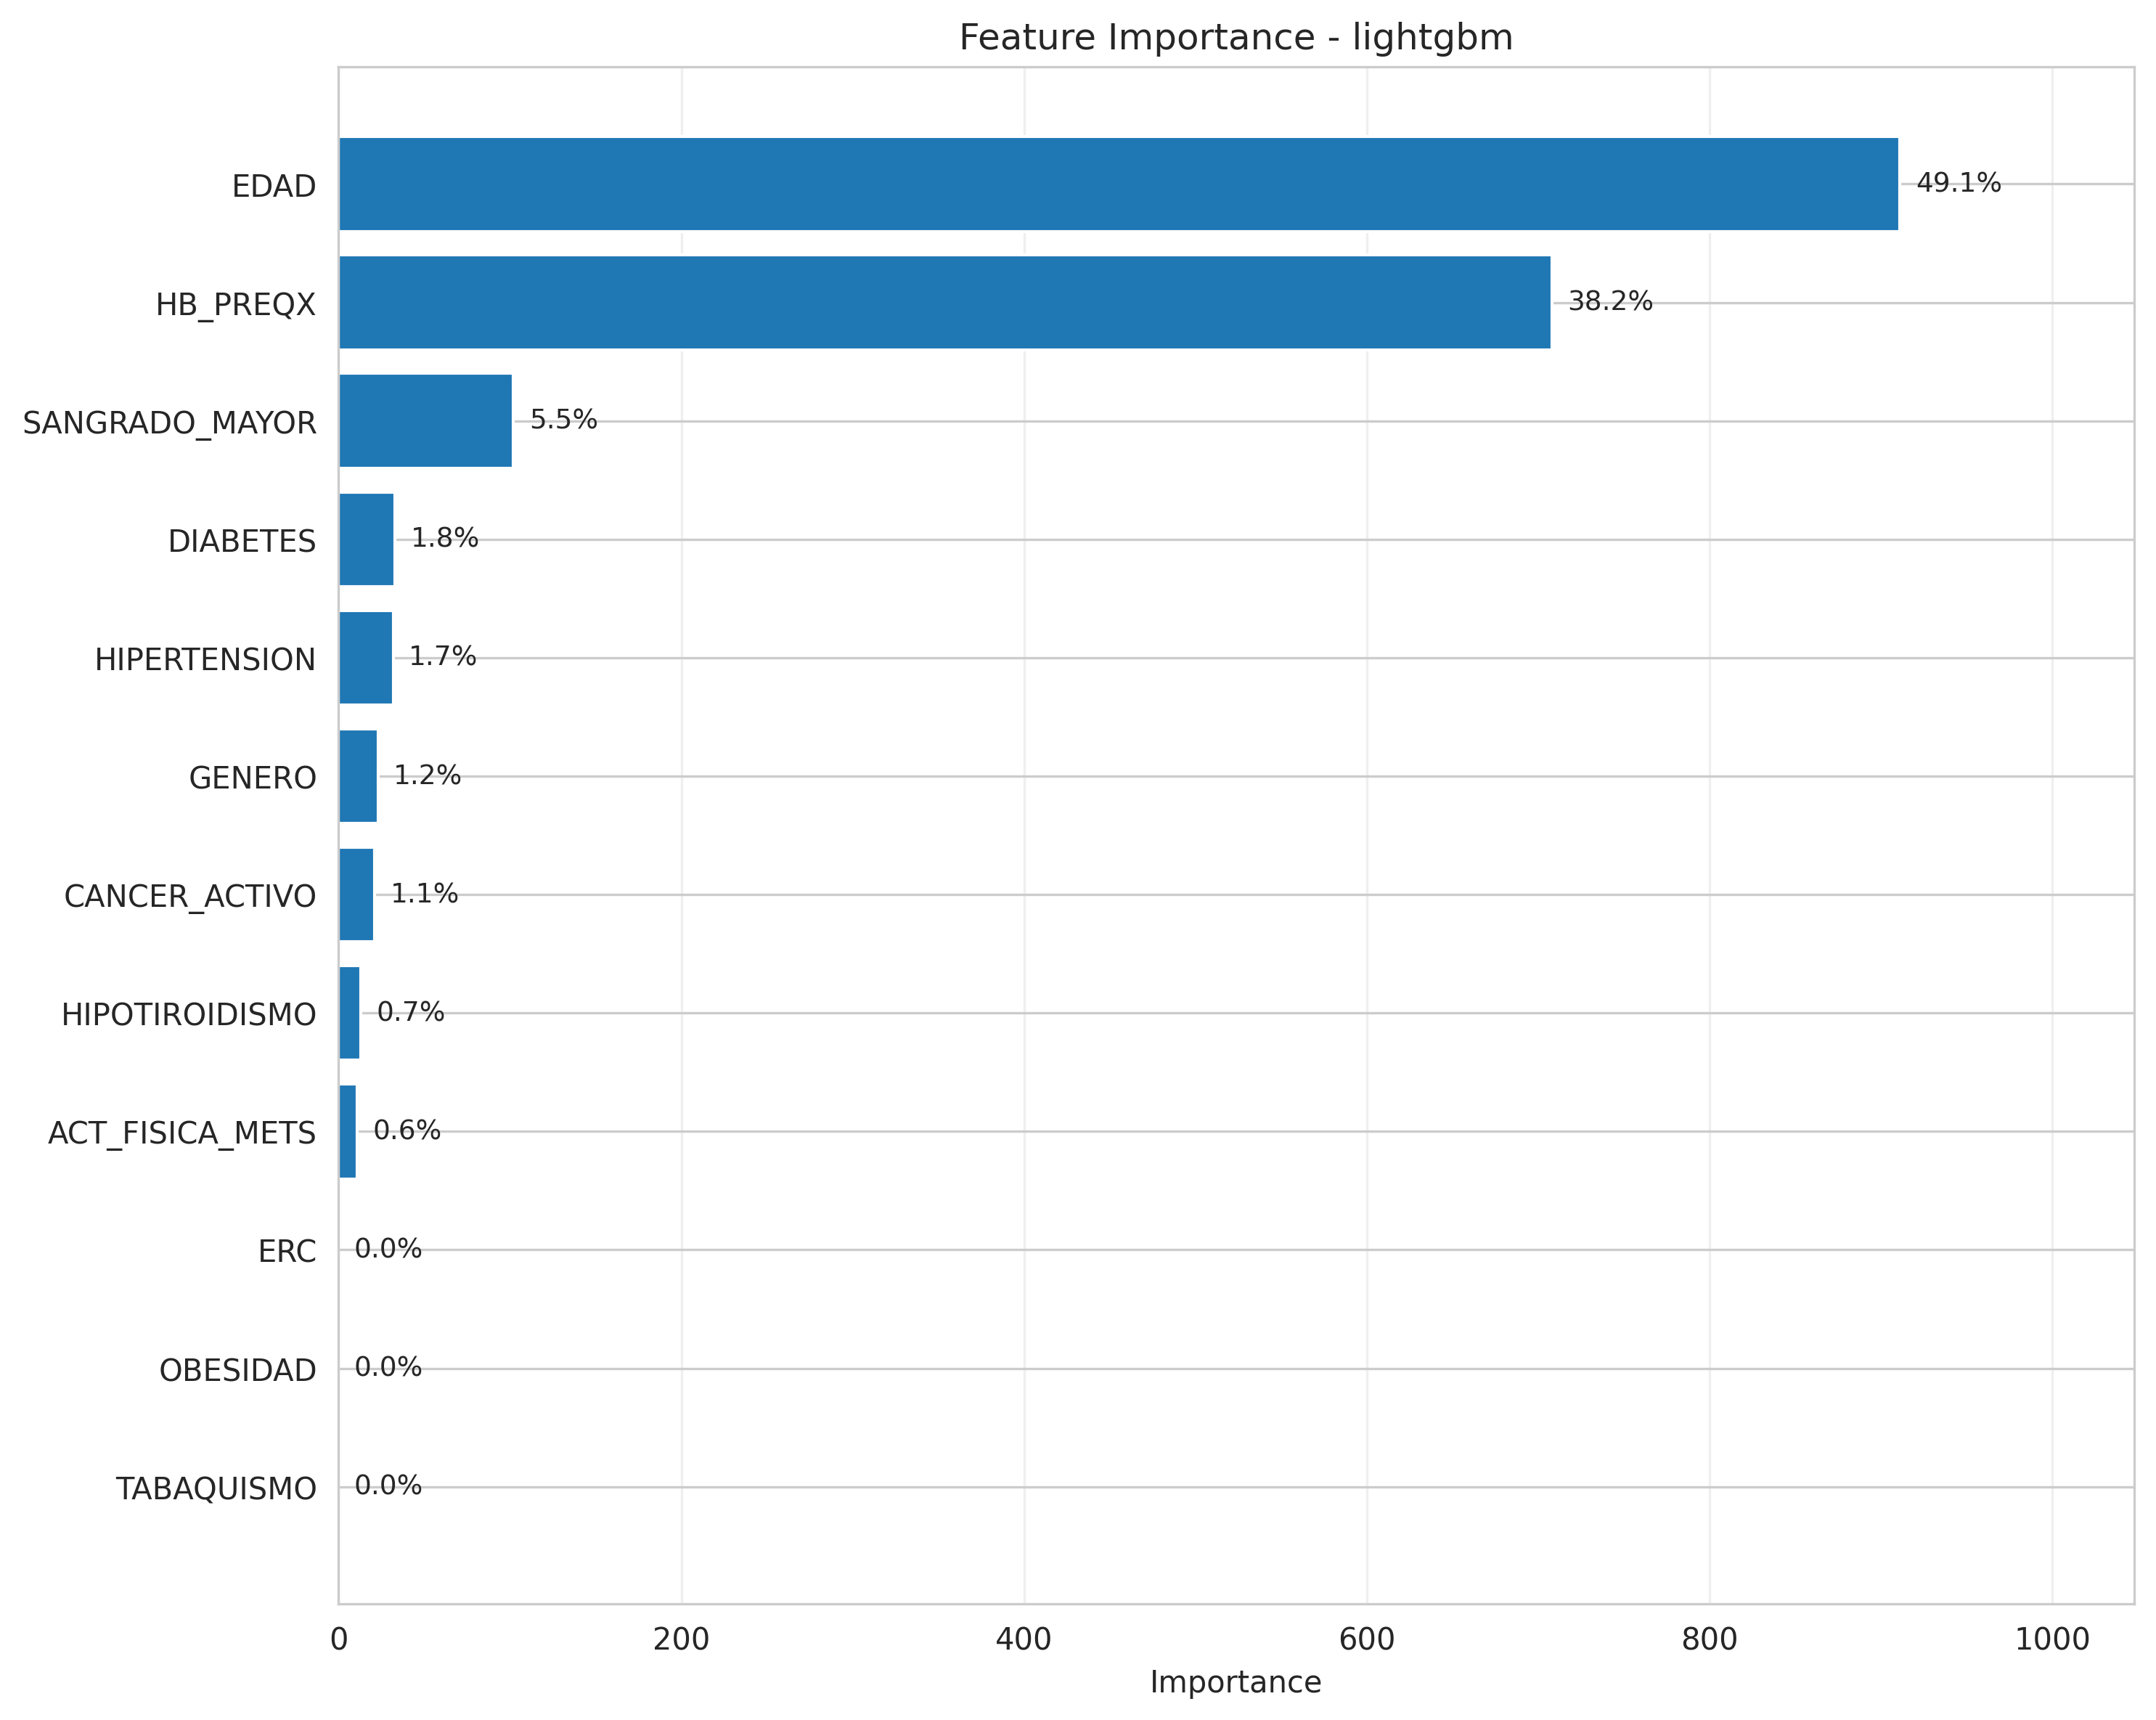
\includegraphics[width=0.85\textwidth]{images/exp_feature_importance.png}
\caption{Importancia de características del modelo LightGBM seleccionado.}
\label{fig:feature-importance-final}
\end{figure}

\begin{figure}[H]
\centering
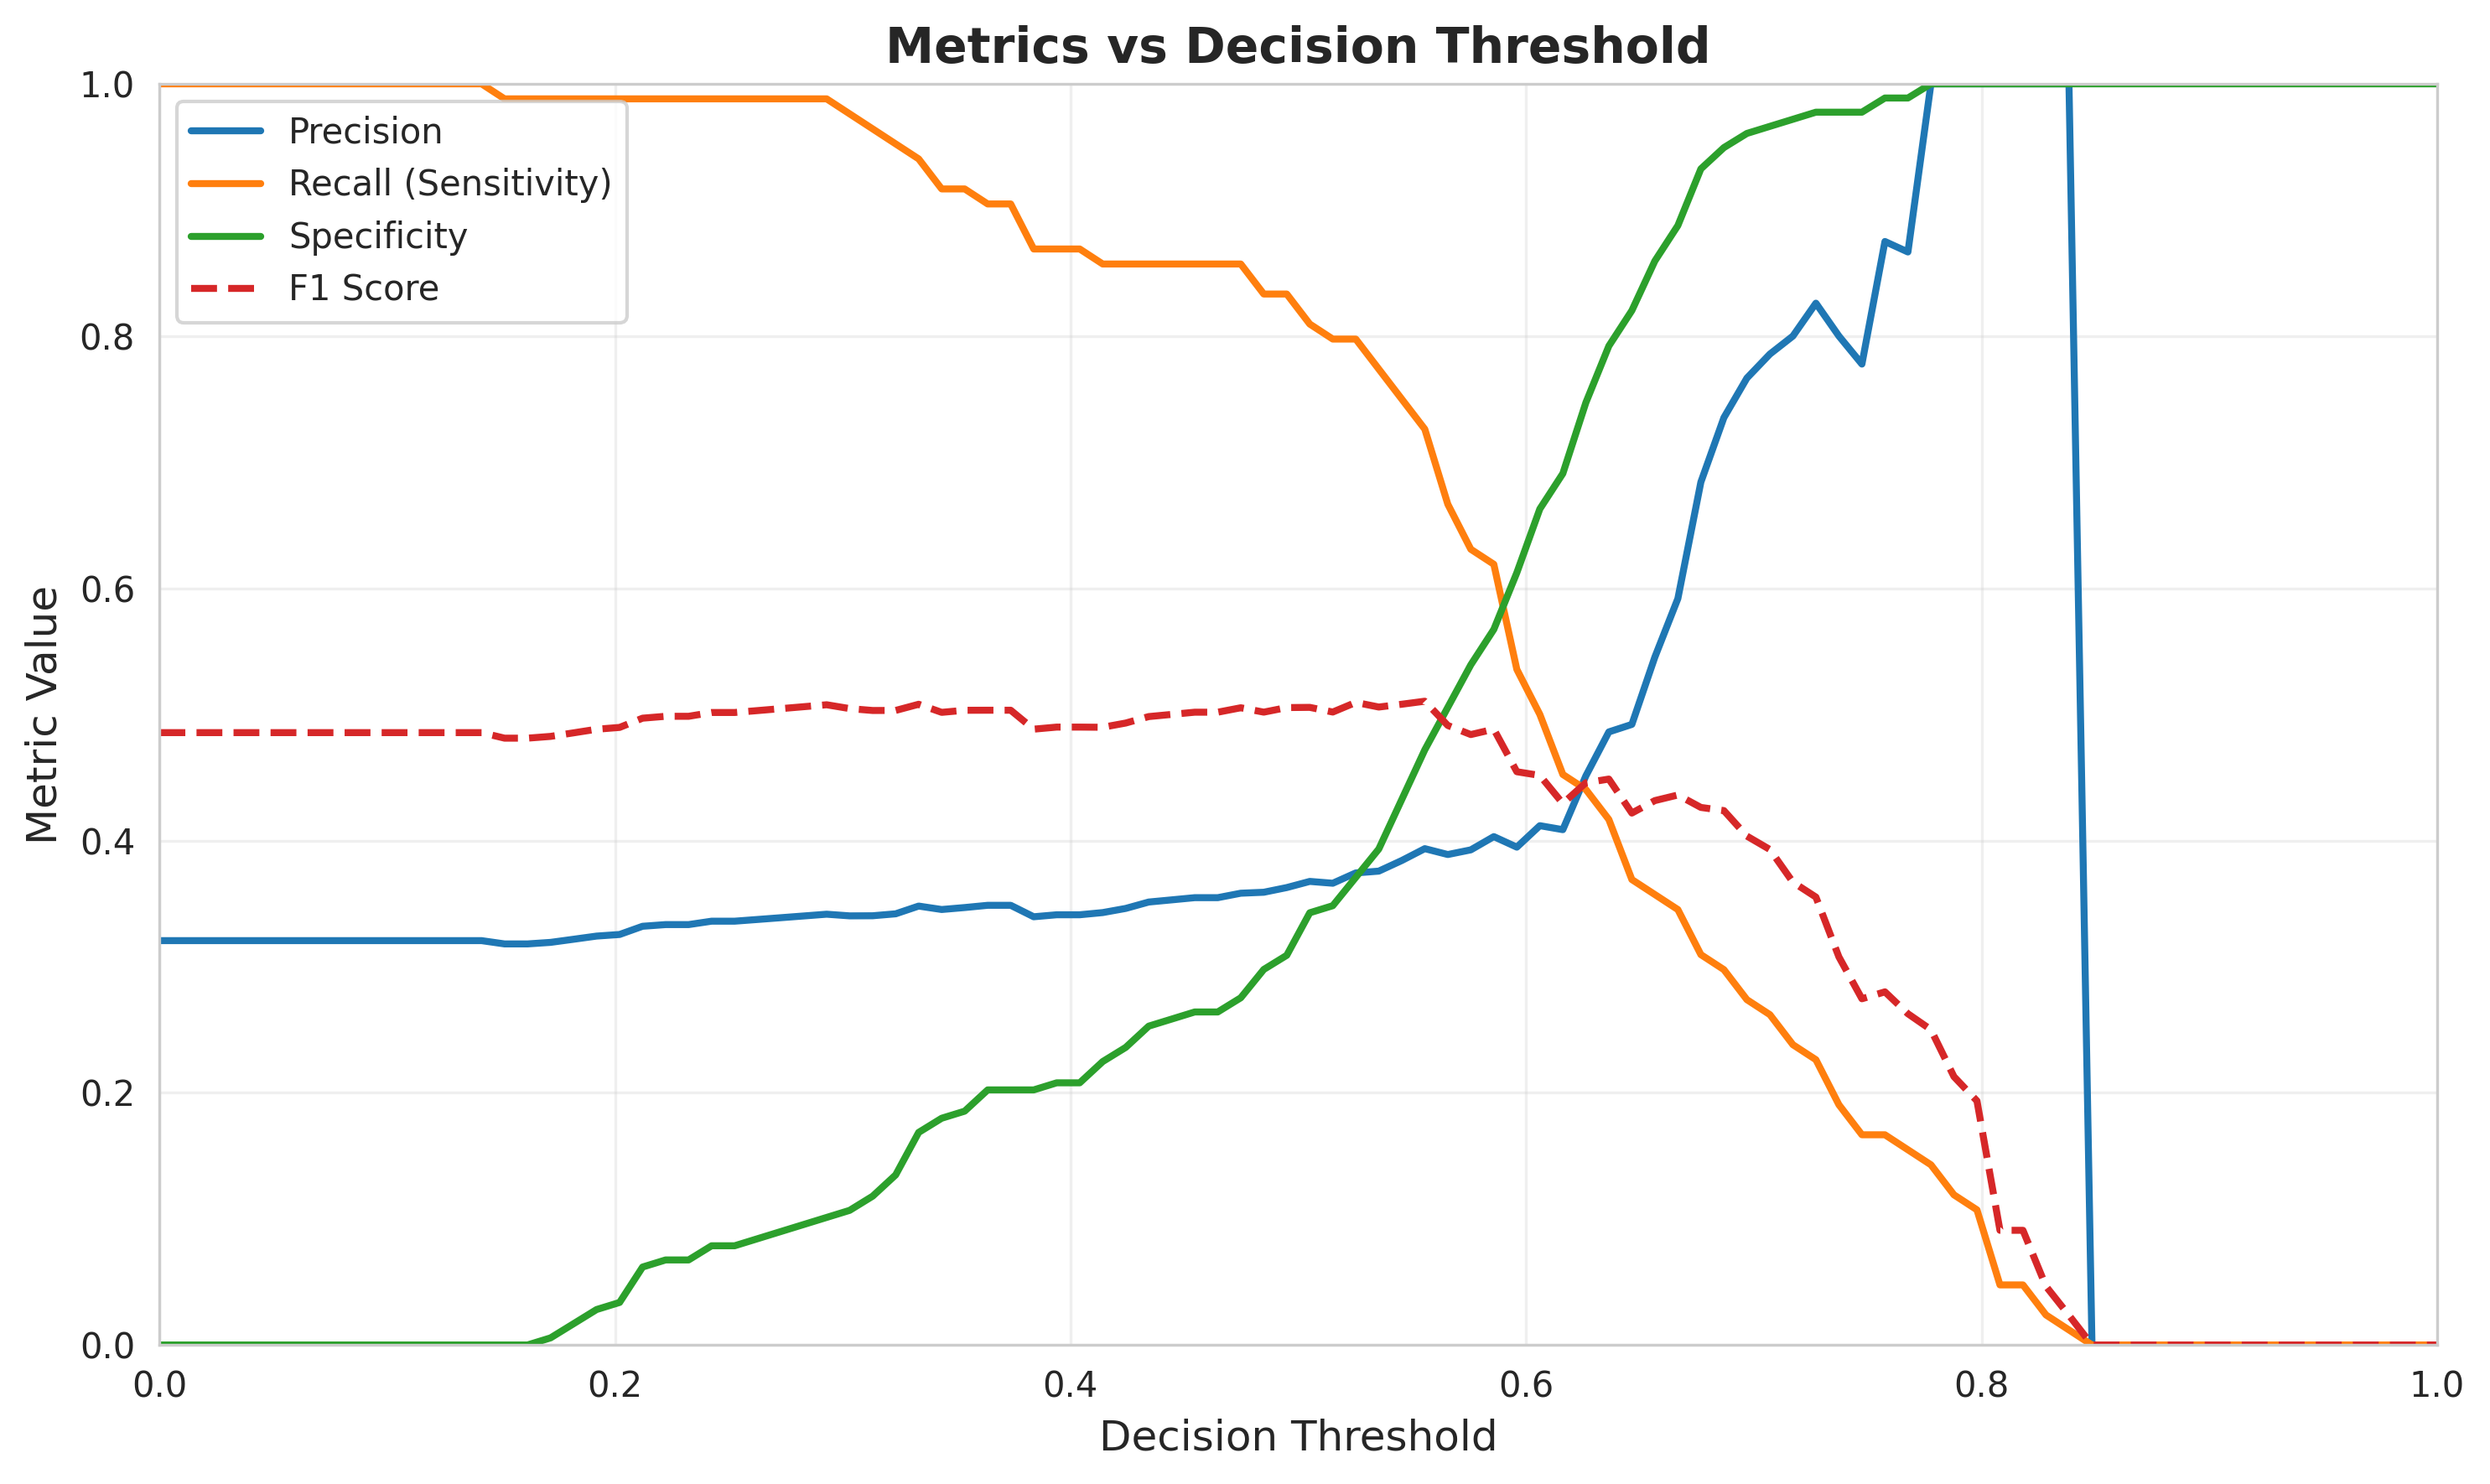
\includegraphics[width=0.85\textwidth]{images/exp_threshold_analysis.png}
\caption{Análisis de umbral de decisión mostrando el trade-off entre métricas según el punto de corte.}
\label{fig:threshold-final}
\end{figure}

\newpage

% -----------------------------------------------------------------------------
% 6. CONCLUSIONES Y FUTURO TRABAJO
% -----------------------------------------------------------------------------
\section{Conclusiones y futuro trabajo}

\subsection{Conclusiones}

El desarrollo de este proyecto permitió explorar exhaustivamente la viabilidad de predecir el shock hemorrágico postoperatorio en pacientes sometidos a cirugía mayor no cardíaca mediante técnicas de inteligencia artificial. A partir de los 19 experimentos realizados, se obtuvieron las siguientes conclusiones:

\begin{enumerate}
    \item \textbf{Limitaciones del dataset preoperatorio:} Las características preoperatorias disponibles (edad, hemoglobina prequirúrgica, comorbilidades) poseen capacidad predictiva limitada cuando se utilizan de forma aislada. El mejor AUC-ROC alcanzado sin información intraoperatoria fue de 0.58, lo cual representa una mejora marginal sobre la clasificación aleatoria.
    
    \item \textbf{Importancia crítica de SANGRADO\_MAYOR:} La inclusión de esta variable intraoperatoria elevó el AUC-ROC a 0.653, representando la mejora más significativa de todos los experimentos. Este hallazgo confirma que la detección temprana del shock requiere información del contexto quirúrgico, no solo factores preoperatorios.
    
    \item \textbf{Variables clave identificadas:} El análisis SHAP identificó que EDAD (42.9\%) y HB\_PREQX (32.8\%) concentran más del 75\% de la importancia predictiva. Esto es clínicamente coherente: pacientes mayores tienen menor capacidad compensatoria y niveles bajos de hemoglobina indican menor reserva ante pérdidas sanguíneas.
    
    \item \textbf{Ingeniería de características limitada:} Ni la categorización de variables continuas ni las agregaciones de comorbilidades mejoraron el rendimiento predictivo. Este resultado está alineado con las conclusiones de Ma et al.\ \cite{ma2023}, quienes documentan que la categorización de predictores continuos reduce la precisión en modelos de predicción clínica, ya que introduce pérdida de información sobre la distribución real de cada variable.
    
    \item \textbf{Comparación de algoritmos:} Se evaluaron seis algoritmos diferentes (Regresión Logística, Random Forest, Gradient Boosting, KNN, LightGBM, Decision Tree y Naive Bayes). LightGBM mostró el mejor rendimiento general, mientras que Decision Tree ofreció el mejor balance entre rendimiento e interpretabilidad clínica.
    
    \item \textbf{Optimización para contexto clínico:} Dado que la consecuencia de no detectar un shock es potencialmente fatal \cite{cannon2018}, se priorizó la maximización del recall sobre otras métricas. El umbral óptimo identificado (0.54) ofrece un recall de 94.3\%, aceptando una especificidad de 27.2\%. Sin embargo, esta baja especificidad implica que aproximadamente 7 de cada 10 alertas serán falsas alarmas, lo que podría generar ``fatiga de alertas'' en el personal médico. Como advierte Steyerberg et al.\ \cite{steyerberg2018}, los resultados favorables del análisis estadístico pueden no traducirse directamente al rendimiento clínico real, por lo que este trade-off debe comunicarse claramente al equipo clínico durante la implementación.
    
    \item \textbf{Interpretabilidad como requisito:} El análisis SHAP y la evaluación de modelos interpretables (Decision Tree) demostraron que es posible proporcionar explicaciones clínicamente significativas de las predicciones, facilitando la adopción del modelo en entornos hospitalarios.
\end{enumerate}

\subsection{Limitaciones del estudio}

\begin{itemize}
    \item \textbf{Definición de la variable objetivo:} La variable objetivo (shock hemorrágico) fue definida mediante el Índice de Shock (IS = FC/PAS) calculado automáticamente y validado por evaluación clínica. Es importante reconocer que el modelo está aprendiendo a replicar este criterio diagnóstico, no necesariamente a predecir el estado fisiopatológico subyacente.
    
    \item \textbf{Tamaño del dataset:} Con 1,307 registros después de limpieza, el dataset es relativamente pequeño para técnicas avanzadas de deep learning. Como señalan Steyerberg et al.\ \cite{steyerberg2018}, esperar generalización amplia a partir de datasets reducidos es una de las principales fuentes de riesgo en el desarrollo de modelos predictivos clínicos. Esta limitación favorece modelos más simples con menor riesgo de sobreajuste.
    
    \item \textbf{Desbalance de clases y SMOTE:} La proporción 2.1:1 entre casos negativos y positivos requirió técnicas de balanceo (SMOTE, class weights). El sobremuestreo sintético en datasets pequeños puede crear patrones artificiales, lo cual explica parcialmente los altos valores de recall con baja especificidad observados en algunos experimentos.
    
    \item \textbf{Manejo de variables continuas:} Los experimentos de categorización de EDAD y HB\_PREQX no produjeron mejoras en el rendimiento. Este resultado está en línea con la revisión sistemática de Ma et al.\ \cite{ma2023}, que demuestra que la dicotomización y categorización de predictores continuos conlleva pérdida de información y reduce la precisión de los modelos de predicción clínica. En nuestro caso, el tratamiento de estas variables como continuas resultó más apropiado.
    
    \item \textbf{Fuentes de datos unimodales:} A diferencia de enfoques como ShockModes \cite{pal2022}, que combina notas clínicas, series temporales de signos vitales y comorbilidades, este proyecto cuenta únicamente con variables tabulares estáticas. La ausencia de variables dinámicas (signos vitales en tiempo real, tendencias de presión arterial) limita la capacidad predictiva del modelo, ya que el shock hemorrágico es un proceso evolutivo que no se captura completamente con datos estáticos.
    
    \item \textbf{Validación externa:} El modelo no fue validado en poblaciones externas a la Fundación Valle del Lili, lo que limita la generalización de los resultados a otras instituciones o poblaciones.
    
    \item \textbf{Fatiga de alertas:} La especificidad de 0.272 (umbral optimizado) implica una alta tasa de falsas alarmas. En entornos clínicos reales, esto puede llevar a que el personal médico ignore progresivamente las alertas del sistema, reduciendo su utilidad práctica.
    
    \item \textbf{Discrepancia entre validación cruzada y conjunto de prueba:} Los valores moderados de AUC-ROC en validación cruzada (0.597) son coherentes con la advertencia de Steyerberg et al.\ \cite{steyerberg2018} sobre la sobreestimación de resultados estadísticos en evaluación interna. Sin embargo, la optimización del umbral permitió obtener una mejora tangible en el conjunto de prueba, lo que sugiere que la estrategia de ajuste del punto de corte puede compensar parcialmente las limitaciones del dataset.
\end{itemize}

\subsection{Trabajo futuro}

\begin{enumerate}
    \item \textbf{Incorporación de variables temporales:} Integrar señales vitales continuas (frecuencia cardíaca, presión arterial, saturación de oxígeno) para capturar tendencias y patrones de deterioro hemodinámico.
    
    \item \textbf{Modelos de series temporales:} Dado que el shock hemorrágico es un proceso evolutivo y no un evento estático, explorar arquitecturas como LSTM (Long Short-Term Memory) o Transformers permitiría modelar la evolución temporal del estado del paciente durante y después de la cirugía.
    
    \item \textbf{Optimización de umbral dinámico:} Investigar umbrales adaptativos que ajusten la sensibilidad según el contexto clínico (tipo de cirugía, perfil de riesgo del paciente) para reducir la fatiga de alertas sin comprometer la detección de casos críticos.
    
    \item \textbf{Validación prospectiva:} Implementar un estudio prospectivo para evaluar el rendimiento del modelo en condiciones clínicas reales y medir el impacto en los tiempos de respuesta del equipo médico.
    
    \item \textbf{Integración con sistemas hospitalarios:} Desarrollar la interfaz de integración con los sistemas de información quirúrgica de la FVL para alertas en tiempo real, incluyendo capacitación al personal sobre cómo interpretar y actuar ante las alertas.
    
    \item \textbf{Ampliación del dataset:} Colaborar con otras instituciones para aumentar el tamaño y diversidad del conjunto de datos, mejorando la generalización del modelo y permitiendo técnicas más avanzadas.
    
    \item \textbf{Predicción conformal:} Implementar técnicas de predicción conformal para proporcionar intervalos de confianza calibrados en las predicciones, aumentando la confiabilidad clínica y permitiendo al médico evaluar la incertidumbre del modelo.
\end{enumerate}

\newpage

% -----------------------------------------------------------------------------
% ANEXOS
% -----------------------------------------------------------------------------
\section*{Anexos}
\addcontentsline{toc}{section}{Anexos}

\subsection*{Árbol de problemas}
\addcontentsline{toc}{subsection}{Árbol de problemas}

\textbf{Problema Principal:}

\vspace{0.3cm}
Detección tardía del riesgo de shock hemorrágico en pacientes sometidos a cirugía mayor no cardiaca postoperatoria

\vspace{0.5cm}
\textbf{Causas:}

\begin{itemize}
    \item \textbf{Causa 1: Dependencia exclusiva de la experiencia médica}
    \begin{itemize}
        \item Sub-causa 1: Variabilidad en la interpretación clínica
        \begin{itemize}
            \item Sub-sub-causa 1: Diferencias en criterios diagnósticos entre profesionales
            \item Sub-sub-causa 2: Falta de protocolos estandarizados de evaluación
        \end{itemize}
        \item Sub-causa 2: Sesgos cognitivos en la toma de decisiones clínicas
        \item Sub-causa 3: Limitaciones humanas en el monitoreo continuo
        \begin{itemize}
            \item Sub-sub-causa 1: Fatiga del personal médico durante procedimientos prolongados
            \item Sub-sub-causa 2: Dificultad para detectar cambios sutiles en signos vitales
            \item Sub-sub-causa 3: Sobrecarga de información durante situaciones críticas
        \end{itemize}
    \end{itemize}
    
    \item \textbf{Causa 2: Protocolos clínicos no actualizados}
    \begin{itemize}
        \item Sub-causa 1: Enfoque reactivo en lugar de predictivo
        \item Sub-causa 2: Criterios diagnósticos basados en manifestaciones tardías
        \item Sub-causa 3: No consideración de factores de riesgo individuales
    \end{itemize}
    
    \item \textbf{Causa 3: Escasa personalización según características del paciente}
    \begin{itemize}
        \item Sub-causa 1: Ignorancia de comorbilidades específicas
        \item Sub-causa 2: Falta de adaptación a características demográficas
    \end{itemize}
\end{itemize}

\vspace{0.5cm}
\textbf{Efectos:}

\begin{itemize}
    \item \textbf{Efecto 1: Aumento de la mortalidad postoperatoria}
    \begin{itemize}
        \item Sub-efecto 1: Muertes por hemorragia no controlada
        \item Sub-efecto 2: Daño irreversible a órganos por hipoperfusión prolongada
        \item Sub-efecto 3: Mayor riesgo de infecciones postoperatorias
        \item Sub-efecto 4: Falla multiorgánica por manejo tardío
    \end{itemize}
    
    \item \textbf{Efecto 2: Mayor necesidad de transfusiones sanguíneas}
    \begin{itemize}
        \item Sub-efecto 1: Uso ineficiente de recursos sanguíneos
        \begin{itemize}
            \item Sub-sub-efecto 1: Transfusiones reactivas en lugar de preventivas
            \item Sub-sub-efecto 2: Escasez de hemoderivados en momentos críticos
            \item Sub-sub-efecto 3: Mayor riesgo de reacciones adversas
        \end{itemize}
        \item Sub-efecto 2: Complicaciones asociadas a transfusiones
        \begin{itemize}
            \item Sub-sub-efecto 1: Sobrecarga circulatoria
            \item Sub-sub-efecto 2: Reacciones inmunológicas
            \item Sub-sub-efecto 3: Mayor riesgo de infecciones
        \end{itemize}
    \end{itemize}
    
    \item \textbf{Efecto 3: Incremento de complicaciones postoperatorias}
    \begin{itemize}
        \item Sub-efecto 1: Daño orgánico por hipoperfusión prolongada
        \begin{itemize}
            \item Sub-sub-efecto 1: Insuficiencia renal aguda
            \item Sub-sub-efecto 2: Daño cerebral por hipoxia
            \item Sub-sub-efecto 3: Necrosis intestinal
        \end{itemize}
        \item Sub-efecto 2: Prolongación de la recuperación
        \begin{itemize}
            \item Sub-sub-efecto 1: Necesidad de cirugías adicionales correctivas
            \item Sub-sub-efecto 2: Rehabilitación más compleja y prolongada
        \end{itemize}
    \end{itemize}
    
    \item \textbf{Efecto 4: Impacto económico y en recursos hospitalarios}
    \begin{itemize}
        \item Sub-efecto 1: Aumento de los costos médicos
        \begin{itemize}
            \item Sub-sub-efecto 1: Mayor duración de la estancia hospitalaria
            \item Sub-sub-efecto 2: Uso excesivo de recursos críticos (UCI, sangre, medicamentos)
            \item Sub-sub-efecto 3: Costos adicionales por manejo de complicaciones
        \end{itemize}
        \item Sub-efecto 2: Saturación de recursos hospitalarios
    \end{itemize}
\end{itemize}

\newpage

\subsection*{Cronograma}
\addcontentsline{toc}{subsection}{Cronograma}

\begin{figure}[H]
\centering
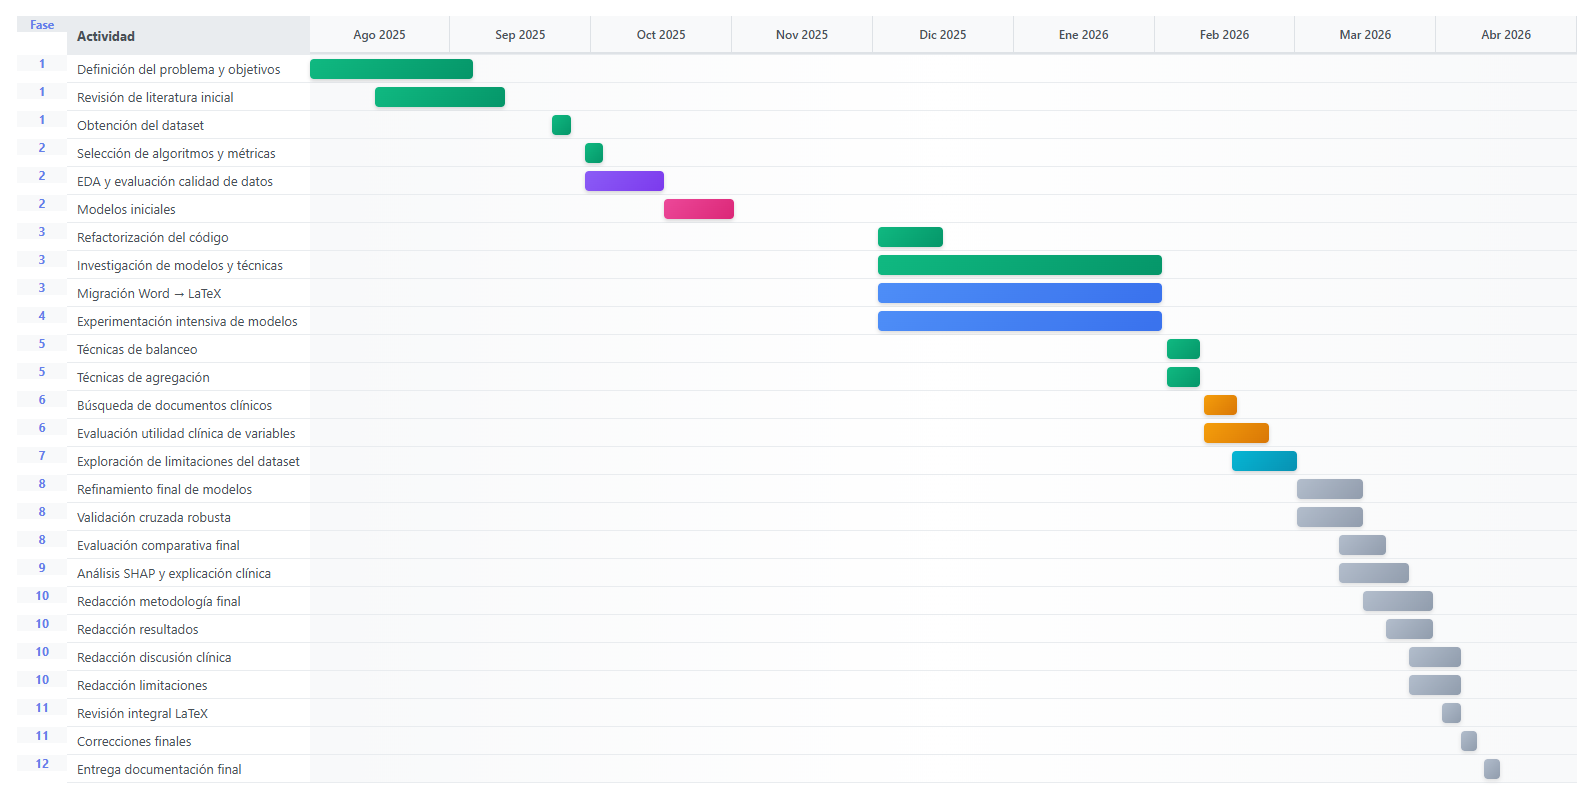
\includegraphics[width=\textwidth]{images/image025.png}
\caption{Cronograma detallado del Proyecto de Grado en Inteligencia Artificial, elaborado mediante TeamGantt}
\end{figure}

\subsection*{Análisis de Participación}
\addcontentsline{toc}{subsection}{Análisis de Participación}

\begin{itemize}
    \item Gustavo Adolfo Cruz Suarez -- Médico Anestesiólogo (FVL)
    \item Daniela Hincapié -- Médico Centro de Investigaciones Clínicas (FVL)
    \item Felipe Ocampo Osorio -- Director de IA (FVL)
\end{itemize}

\newpage

% -----------------------------------------------------------------------------
% ANEXO: EVOLUCIÓN DE EXPERIMENTOS
% -----------------------------------------------------------------------------
\subsection*{Evolución de Experimentos}
\addcontentsline{toc}{subsection}{Evolución de Experimentos}

Se realizaron cinco experimentos para optimizar la predicción del shock hemorrágico. A continuación se presenta la evolución de los modelos evaluados, destacando las mejoras progresivas en AUC-ROC.

\subsubsection*{Experimento 1: Modelos Base}

\textbf{Descripción:} Evaluación inicial de siete algoritmos de machine learning con el conjunto de datos original.

\textbf{Mejor modelo:} \expOneBestModel

\textbf{AUC-ROC (CV):} \expOneAUC

\textbf{Resultados comparativos:}

\begin{figure}[H]
\centering
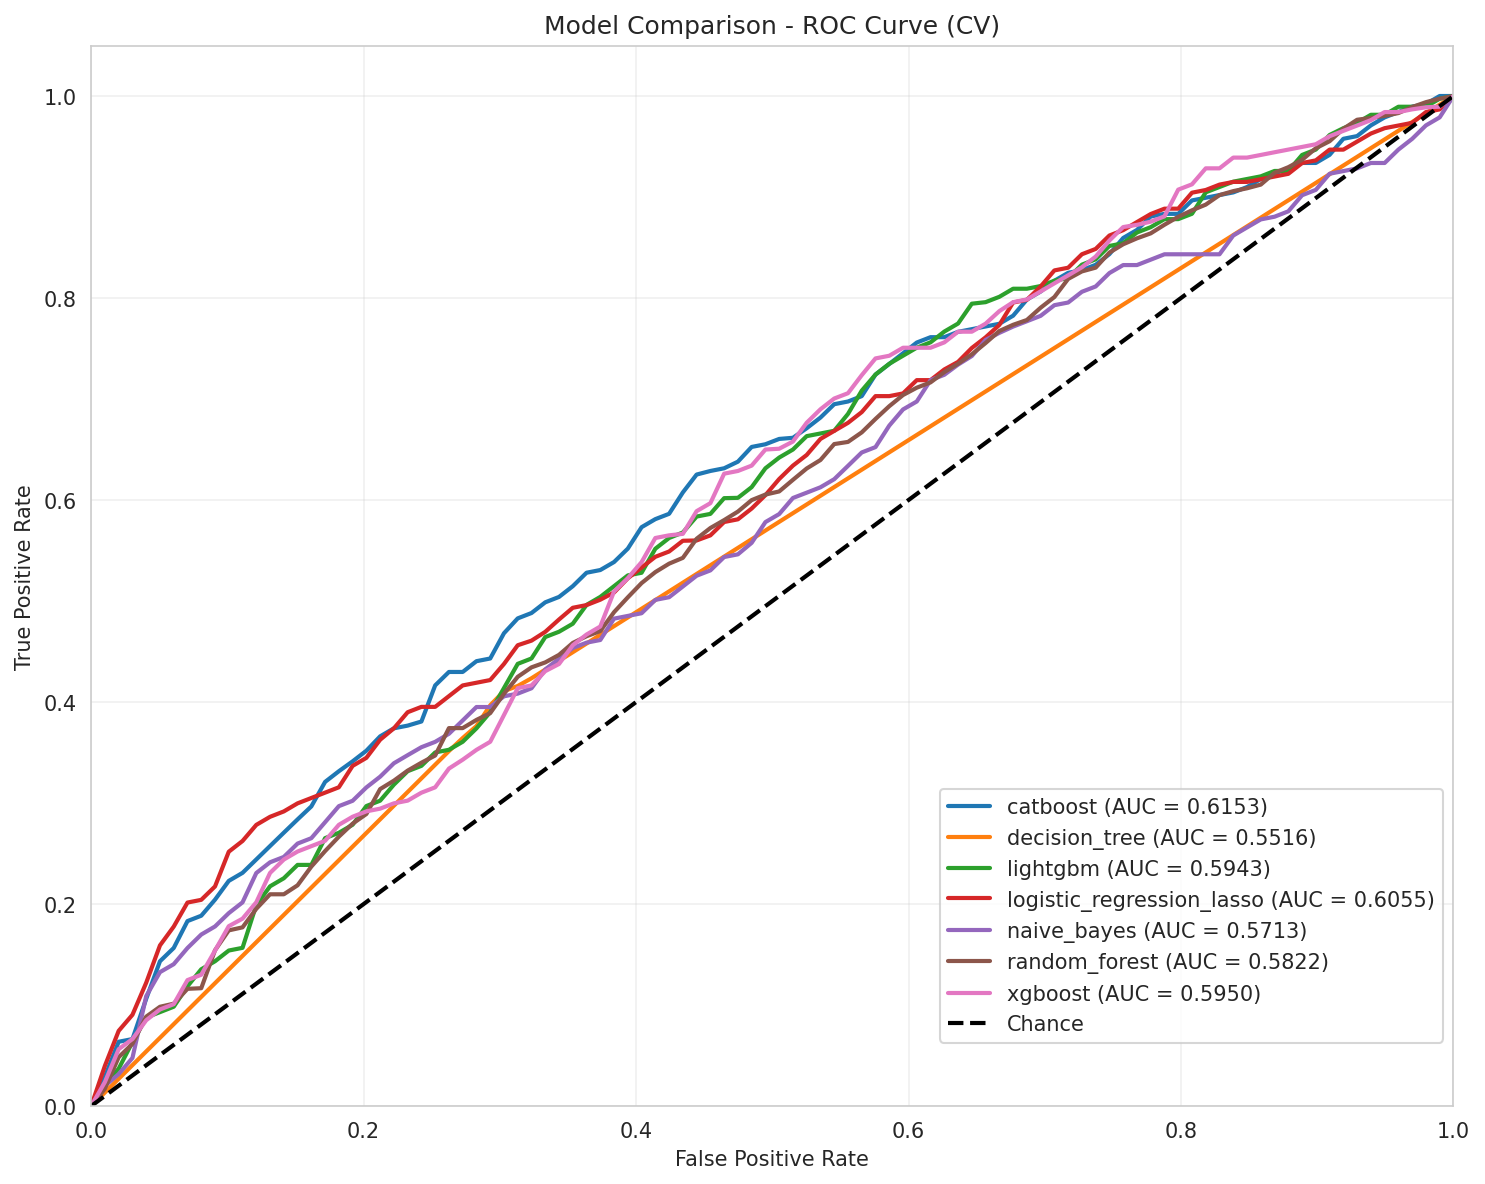
\includegraphics[width=0.85\textwidth]{../experiments/exp_01_base_models/comparison_plots/roc_comparison.png}
\caption{Comparación de curvas ROC - Experimento 1}
\end{figure}

\subsubsection*{Experimento 2: Características Agregadas}

\textbf{Descripción:} Introducción de variables derivadas: EDAD\textsuperscript{2}, HB\_x\_SANGRADO, síndromes agregados (cardiovascular, metabólico, pulmonar).

\textbf{Mejor modelo:} \expTwoBestModel

\textbf{AUC-ROC (CV):} \expTwoAUC

\textbf{Mejora respecto al Experimento 1:} +0.0082

\begin{figure}[H]
\centering

\includegraphics[width=0.85\textwidth]{../experiments/exp_02_aggregated_features/comparison_plots/roc_comparison.png}
\caption{Comparación de curvas ROC - Experimento 2}
\end{figure}

\subsubsection*{Experimento 3: Características Categóricas}

\textbf{Descripción:} Categorización de variables continuas (EDAD, HB\_PREQX) en rangos clínicos.

\textbf{Mejor modelo:} \expThreeBestModel

\textbf{AUC-ROC (CV):} \expThreeAUC

\textbf{Resultado:} Disminución de rendimiento (-0.0101 vs Exp 2), confirmando que la categorización reduce la precisión predictiva.

\begin{figure}[H]
\centering

\includegraphics[width=0.85\textwidth]{../experiments/exp_03_categorical_features/comparison_plots/roc_comparison.png}
\caption{Comparación de curvas ROC - Experimento 3}
\end{figure}

\subsubsection*{Experimento 4: Poda de Características}

\textbf{Descripción:} Selección de características basada en importancia (eliminación de variables con bajo impacto predictivo).

\textbf{Mejor modelo:} \expFourBestModel

\textbf{AUC-ROC (CV):} \expFourAUC

\textbf{Mejora respecto al Experimento 3:} +0.0075

\begin{figure}[H]
\centering

\includegraphics[width=0.85\textwidth]{../experiments/exp_04_feature_pruning/comparison_plots/roc_comparison.png}
\caption{Comparación de curvas ROC - Experimento 4}
\end{figure}

\subsubsection*{Experimento 5: Búsqueda de Hiperparámetros (Modelo Campeón)}

\textbf{Descripción:} Optimización exhaustiva de hiperparámetros mediante GridSearchCV para todos los modelos.

\textbf{Mejor modelo:} \championModelName

\textbf{AUC-ROC (CV):} \championROCAUC

\textbf{Mejora respecto al Experimento 1:} +0.0238 (mejora del 3.9\%)

\begin{figure}[H]
\centering

\includegraphics[width=0.85\textwidth]{../experiments/exp_05_hyperparameter_search/comparison_plots/roc_comparison.png}
\caption{Comparación de curvas ROC - Experimento 5 (Modelo Campeón)}
\end{figure}

\subsubsection*{Métricas del Modelo Campeón (Conjunto de Prueba)}

El modelo \championModelName\ del Experimento 5 fue seleccionado como modelo campeón por presentar el mejor balance entre Recall (\championRecall) y F2-Score (\championFTwoScore).

\begin{table}[H]
\centering
\caption{Métricas del Modelo Campeón - \championModelName\ (Experimento 5)}
\begin{tabular}{|l|r|}
\hline
\textbf{Métrica} & \textbf{Valor} \\ \hline
AUC-ROC (CV) & \championROCAUC \\ \hline
Brier Score & \championBrierScore \\ \hline
Recall (Sensibilidad) & \championRecall \\ \hline
Especificidad & \championSpecificity \\ \hline
Precisión & \championPrecision \\ \hline
Valor Predictivo Negativo (NPV) & \championNPV \\ \hline
F1-Score & \championFOneScore \\ \hline
F2-Score & \championFTwoScore \\ \hline
Accuracy & \championAccuracy \\ \hline
Kappa de Cohen & \championKappa \\ \hline
Umbral Óptimo & \championOptimalThreshold \\ \hline
\end{tabular}
\end{table}

\textbf{Interpretación clínica:}

\begin{itemize}
    \item \textbf{Recall de \championRecall:} El modelo detecta \championTPpct\% de los casos de shock hemorrágico, cumpliendo el objetivo de maximizar la detección temprana.

    \item \textbf{NPV de \championNPV:} Cuando el modelo predice ausencia de shock, tiene una confianza del \championNPV, lo cual es crucial para reducir intervenciones innecesarias.

    \item \textbf{Especificidad de \championSpecificity:} La baja especificidad implica una tasa de falsos positivos del \championFPpct\%, lo que debe ser comunicado al equipo clínico para evitar fatiga de alertas.

    \item \textbf{F2-Score de \championFTwoScore:} Métrica que pondera más el Recall que la Precisión, alineada con el objetivo clínico de priorizar la detección de casos positivos.
\end{itemize}

\subsubsection*{Características Más Importantes}

Las tres variables con mayor importancia predictiva en el modelo campeón son:

\begin{enumerate}
    \item \textbf{\topFeatureOne:} \topFeatureOneImportance\%
    \item \textbf{\topFeatureTwo:} \topFeatureTwoImportance\%
    \item \textbf{\topFeatureThree:} \topFeatureThreeImportance\%
\end{enumerate}

\begin{figure}[H]
\centering

\includegraphics[width=0.85\textwidth]{../experiments/exp_05_hyperparameter_search/models/xgboost/plots/feature_importance.png}
\caption{Importancia de características - Modelo Campeón (\championModelName)}
\end{figure}

\subsubsection*{Curvas de Calibración}

\begin{figure}[H]
\centering

\includegraphics[width=0.85\textwidth]{../experiments/exp_05_hyperparameter_search/models/xgboost/plots/calibration_curve_cv.png}
\caption{Curva de calibración - Modelo Campeón}
\end{figure}

\subsubsection*{Matriz de Confusión}

\begin{figure}[H]
\centering

\includegraphics[width=0.85\textwidth]{../experiments/exp_05_hyperparameter_search/models/xgboost/plots/confusion_matrix_normalized.png}
\caption{Matriz de confusión - Modelo Campeón (Umbral: \championOptimalThreshold)}
\end{figure}

\newpage

\begin{thebibliography}{99}
\addcontentsline{toc}{subsection}{Referencias}

\bibitem{bonanno2023}
F. G. Bonanno, ``Management of Hemorrhagic Shock: Physiology Approach, Timing and Strategies,'' Jan. 01, 2023, MDPI. doi: 10.3390/jcm12010260.

\bibitem{terceros2017}
L. J. Terceros-Almanza et al., ``Prediction of massive bleeding. Shock index and modified shock index,'' \textit{Medicina Intensiva (English Edition)}, vol. 41, no. 9, pp. 532--538, Dec. 2017, doi: 10.1016/J.MEDINE.2017.10.003.

\bibitem{moll2025}
V. Moll, A. K. Khanna, and P. Mathur, ``Artificial intelligence for the prediction of postoperative complications in the critically ill,'' \textit{Critical Care Science}, vol. 37, p. e20250025, 2025, doi: 10.62675/2965-2774.20250025.

\bibitem{hooper2022}
N. Hooper and T. J. Armstrong, ``Hemorrhagic Shock,'' \textit{StatPearls}, Sep. 2022, Accessed: Sep. 07, 2025. [Online]. Available: \url{https://www.ncbi.nlm.nih.gov/books/NBK470382/}

\bibitem{james2023}
G. James, D. Witten, T. Hastie, R. Tibshirani, and J. Taylor, ``An Introduction to Statistical Learning,'' 2023, doi: 10.1007/978-3-031-38747-0.

\bibitem{collins2015}
G. S. Collins, J. B. Reitsma, D. G. Altman, and K. G. M. Moons, ``Transparent reporting of a multivariable prediction model for individual prognosis or diagnosis (TRIPOD): The TRIPOD statement,'' \textit{BMJ (Online)}, vol. 350, Jan. 2015, doi: 10.1136/BMJ.G7594.

\bibitem{zhang2025}
Z. Zhang et al., ``Machine learning model for postpancreaticoduodenectomy haemorrhage prediction: an international multicentre cohort study,'' \textit{BMJ Open}, vol. 15, no. 7, p. e096147, Jul. 2025, doi: 10.1136/BMJOPEN-2024-096147.

\bibitem{cong2025}
X. Cong, X. Zou, R. Zhu, Y. Li, L. Liu, and J. Zhang, ``Development and validation of a machine learning-based model for perioperative stroke prediction in noncardiac, nonvascular, and nonneurosurgical patients,'' \textit{Front Physiol}, vol. 16, p. 1624898, 2025, doi: 10.3389/FPHYS.2025.1624898/FULL.

\bibitem{lucas2019}
A. Lucas, A. T. Williams, and P. Cabrales, ``Prediction of Recovery from Severe Hemorrhagic Shock Using Logistic Regression,'' \textit{IEEE J Transl Eng Health Med}, vol. 7, 2019, doi: 10.1109/JTEHM.2019.2924011.

\bibitem{crispdm1999}
Ncr and J. Clinton, ``CRISP-DM 1.0 Step-by-step data mining guide,'' 1999.

\bibitem{piasta2010}
S. B. Piasta and L. M. Justice, ``Cohen's d Statistic,'' \textit{Encyclopedia of Research Design}, pp. 181--185, May 2010, doi: 10.4135/9781412961288.

\bibitem{wasserstein2016}
R. L. Wasserstein and N. A. Lazar, ``The ASA Statement on p-Values: Context, Process, and Purpose,'' \textit{Am Stat}, vol. 70, no. 2, pp. 129--133, Apr. 2016, doi: 10.1080/00031305.2016.1154108.

\bibitem{allen2017}
M. Allen, ``Cramér's V,'' \textit{The SAGE Encyclopedia of Communication Research Methods}, Jul. 2017, doi: 10.4135/9781483381411.N107.

\bibitem{cannon2018}
J. W. Cannon, ``Hemorrhagic Shock,'' \textit{The New England Journal of Medicine}, vol. 378, no. 4, pp. 370--379, 2018, doi: 10.1056/NEJMra1705649.

\bibitem{ma2023}
J. Ma, P. Dhiman, C. Qi, G. Bullock, M. van Smeden, R. D. Riley, and G. S. Collins, ``Poor handling of continuous predictors in clinical prediction models using logistic regression: A systematic review,'' \textit{Journal of Clinical Epidemiology}, vol. 161, pp. 140--151, 2023, doi: 10.1016/j.jclinepi.2023.07.012.

\bibitem{pal2022}
R. Pal et al., ``ShockModes: A Multimodal Model for Prognosticating Intensive Care Outcomes from Physician Notes and Vitals,'' \textit{medRxiv}, 2022, doi: 10.1101/2022.12.16.22283559.

\bibitem{steyerberg2018}
E. W. Steyerberg, H. Uno, J. P. A. Ioannidis, B. van Calster, and collaborators, ``Clinical prediction models cannot be trusted when common modeling approaches are followed,'' \textit{Journal of Clinical Epidemiology}, vol. 98, pp. 133--143, 2018, doi: 10.1016/j.jclinepi.2018.02.008.

\end{thebibliography}

\end{document}